\documentclass[12pt,a4paper,openright,twoside]{book}
\usepackage[utf8]{inputenc}
\usepackage{phd-thesis}
\usepackage{code-lstlistings}
\usepackage{notes}
\usepackage{shortcuts}
\usepackage{amsmath}
\usepackage{amsthm}
\usepackage{amsfonts}
\usepackage{subcaption}
\usepackage{xcolor}
\usepackage[table]{xcolor}
\usepackage{booktabs}
\usepackage{graphicx}
\usepackage{rotating}
\usepackage{float}
\usepackage{pdflscape} %questo gira le pagine (meglio questo per leggere online)
%\usepackage{lscape} %questo solo le tabelle
\usepackage{algorithm}
\usepackage{algpseudocode}
\usepackage{xspace}
\usepackage{tabularx}
\usepackage{makecell}
\usepackage{tikz}
\usepackage{multirow}
\usepackage{siunitx}
\usepackage{mathrsfs}
\usepackage{hyperref}

% Load natbib before bibentry for full compatibility
\usepackage[numbers,square]{natbib}
\usepackage{bibentry}

%remove bounding boxes around clickable elements
\hypersetup{
	hidelinks
}

%----- Command -----%
% Teniamo la convenzione mathtt = parametri ; mathit = variabili
\newcommand{\wtab}{\mathtt{WTab}}
\newcommand{\htab}{\mathtt{HTab}}
\newcommand{\wmin}{\mathtt{WMin}}
\newcommand{\hmin}{\mathtt{HMin}}
\newcommand{\ntypes}{\mathtt{NTypes}}
\newcommand{\nfix}{\mathtt{NFix}}
\newcommand{\wfix}{\mathtt{WFix}}
\newcommand{\hfix}{\mathtt{HFix}}
\newcommand{\nmin}{\mathtt{NMin}}
\newcommand{\nmax}{\mathtt{NMax}}
\newcommand{\finer}{f_\mathit{iner}}
\newcommand{\fdist}{f_\mathit{dist}}
\newcommand{\fdistsemi}{f_{\mathit{dist}}^{\mathit{semi\text{-}perimeter}}}
\newcommand{\fdistarea}{f_{\mathit{dist}}^{\mathit{area}}}
\newcommand{\numext}{\mathtt{NExt}}
\newcommand{\ehside}{\mathtt{HExt}}
\newcommand{\ewside}{\mathtt{WExt}}
\newcommand{\xext}{\mathtt{XExt}}
\newcommand{\yext}{\mathtt{YExt}}
\newcommand{\used}{\mathit{used}}
\newcommand{\samebar}{\mathit{same\_bar}}
\newcommand{\sametype}{\mathit{same\_type}}
\newcommand{\belowinbar}{\mathit{below\_in\_bar}}
\newcommand{\aboveinbar}{\mathit{above\_in\_bar}}
\newcommand{\nooverlapabove}{\mathit{above}}
\newcommand{\nooverlapbelow}{\mathit{below}}
\newcommand{\nooverlapleft}{\mathit{left}}
\newcommand{\nooverlapright}{\mathit{right}}
\newcommand{\aboveext}{\mathit{above\_ext}}
\newcommand{\belowext}{\mathit{below\_ext}}
\newcommand{\leftext}{\mathit{left\_ext}}
\newcommand{\rightext}{\mathit{right\_ext}}
\newcommand{\xcdiffpos}{\mathit{xc\_diff\_positive}}
\newcommand{\ycdiffpos}{\mathit{yc\_diff\_positive}}
\newcommand{\xcdiff}{\mathit{xc\_diff}}
\newcommand{\ycdiff}{\mathit{yc\_diff}}

\newcommand{\swarmsize}{\mathtt{swarm\_size}}
\newcommand{\maxiter}{\mathtt{max\_iter}}
\newcommand{\nvar}{\mathtt{NVars}}
\newcommand{\lns}{Gecode+LNS\xspace}

\newcommand{\rob}[1]{\textcolor{red}{~\textbf{ROB}: #1}}
\newcommand{\vic}[1]{\textcolor{purple}{~\textbf{VIC}: #1}}
\newcommand{\anna}[1]{\textcolor{blue}{~\textbf{ANNA}: #1}}


\mainlinespacing{1.241} % line spacing in mainmatter, comment to default (1)

\begin{document}
	
	\nobibliography*
	
	\frontmatter
	%!TeX root = phd-thesis.tex
\title{Title}
\author{Candidate Name Here}
\date{\today}

\newgeometry{margin=0.8in}
\begin{titlepage}
	\begin{center}
		% \vspace*{0.2cm}

		\large
		\textbf{ALMA MATER STUDIORUM -- UNIVERSITÀ DI BOLOGNA \\ DISI Dipartimento di Informatica: Scienza e Ingegneria}
		\\
		\noindent\hrulefill
		\vspace{0.4cm}

		\Large
		Dottorato di Ricerca in \\
		Computer Science and Engineering

		\vspace{0.4cm}

		Ciclo XXXIX

		\vspace{0.4cm}

		Settore Scientifico Disciplinare: INF/01

		Settore Concorsuale: 01/B1

		\Huge
		\vspace{3cm}
		\textbf{
			Intelligent Decision Support System for Manufacturing Industry
		}

		{\Large{
		\vspace{3cm}

		\textit{Candidato:\\}
		\centering
		Dott.ssa Anna Vitali}
		\\}
		\large
		\vspace{2.5cm}
		\begin{minipage}[t]{0.64\textwidth}
			\begin{flushleft}
				\textit{Coordinatrice Dottorato:}
				\\
				\textbf{Prof.ssa Paola Salomoni}
			\end{flushleft}
		\end{minipage}
		\begin{minipage}[t]{0.34\textwidth}
			\begin{flushright}
				\textit{Supervisore:}
				\\
				\textbf{Prof.} \textbf{Maurizio Gabbrielli}
				\\
				\vspace{0.4cm}
				\textit{Co-supervisori:}
				\\
				\textbf{Prof.} \textbf{Vittorio Maniezzo}
				\\
				\textbf{Prof.} \textbf{Roberto Amadini}
			\end{flushright}

		\end{minipage}\\

		\vfill
		\noindent\hrulefill
		\vspace{0.3cm}
		\Large

		Esame finale anno 2026
	\end{center}
\end{titlepage}
\restoregeometry
	
	\begin{abstract}
		Recent technological advances in manufacturing have enabled the development of increasingly sophisticated machinery and created new opportunities for integrating Intelligent Decision Support Systems (IDSS) to assist machine operators. However, determining appropriate machine configurations remains challenging, particularly when the underlying physical processes are complex, the number of possible configurations is large, and operational and safety constraints must be satisfied.
		
		This thesis investigates the development of IDSS software for the manufacturing industry, with the objective of supporting operators in optimizing machine configuration tasks. The research was developed in collaboration with an industrial partner and addresses two real-world problems: fixture layout optimization, concerning the positioning and configuration of fixtures used to support workpieces in woodworking, and heating process optimization, concerning the determination of machine parameters required to achieve a desired temperature distribution at the core of the sheet during thermoforming.
		
		The developed approaches demonstrate that integrating different solution strategies can effectively address different aspects of complex industrial problems. In fixture layout optimization, exact optimization techniques formally represent the problem constraints and enable the identification of feasible, high-quality configurations, while local search methods further refine the resulting solutions. In heating process optimization, neural network models trained on data generated by physics-based simulations provide computationally efficient predictions, which are subsequently refined through numerical optimization to improve their accuracy and adaptation to individual cases.
		
		The experimental results obtained on real-world test cases demonstrate the effectiveness of the proposed approaches and their potential to support operators in making machine configuration decisions.
	\end{abstract}
	
	\begin{dedication} % this is optional
		You wish and you dream with all your little heart. \\But you remember, that old star can only take you part of the way. \\You got to help it along with some hard work of your own. \\
		\vspace{0.5em}
		--- Tiana’s father, \textit{The Princess and the Frog} (2009)
	\end{dedication}
	
	%\begin{acknowledgements} % this is optional
	%	Optional. Max 1 page.
	%\end{acknowledgements}
	
	%----------------------------------------------------------------------------------------
	\tableofcontents
	\listoffigures     % (optional) comment if empty
	\listoftables
	\listofalgorithms
	\lstlistoflistings % (optional) comment if empty
	%----------------------------------------------------------------------------------------
	
	\mainmatter
	
	%----------------------------------------------------------------------------------------
	\chapter{General introduction}
	\label{chap:introduction}

Recent technological advances have led manufacturing companies to furnish their machines with increasingly sophisticated sensors and interfaces. At the same time, the widespread adoption of Artificial Intelligence (AI) technologies, particularly Neural Networks (NNs), has encouraged companies to investigate how these methods could improve machine functionalities.

As a result, these technological developments have enabled the creation of more advanced machinery integrating Intelligent Decision Support Systems (IDSS)~\cite{phillips2013intelligent}, capable of assisting operators during manufacturing activities.

Although the machinery produced varies significantly in functionality and features, many manufacturing processes require interaction with a human operator and compliance with operational and safety constraints. During the initial stage of production, the operator typically configures the parameters governing the manufacturing process, while in the final stage the quality of the finished product is evaluated.

The physical processes underlying manufacturing operations directly influence the quality of the final product. However, operators often lack the time or expertise required to analyze these processes in detail and therefore rely on the machine interface to provide guidance and support for decision making.

The objective of this work is to improve the decision-making process of human operators interacting with manufacturing machines by developing Intelligent Decision Support Systems (IDSS) aimed at optimizing the tasks performed during machine configuration.

This doctoral thesis was developed in collaboration with SCM Group S.p.A., an Italian company and world leader in the production of machinery for processing a wide range of materials, including wood, plastic, glass, stone, metal, and composite materials.

The remainder of this thesis investigates two optimization problems arising in industrial machine configuration. The first, referred to as \textit{Fixture Layout Optimization}, addresses the positioning and configuration of fixtures used to support wooden workpieces during machining in a \textit{work center}. The problem is investigated by integrating exact optimization methods with heuristic search techniques to identify feasible, high-quality fixture configurations. This problem is addressed in the first part of the thesis.

The second problem, referred to as \textit{Heating Process Optimization}, concerns the determination of machine parameters required to achieve a target temperature distribution within the core of a plastic sheet in a \textit{thermoforming} machine. The problem is addressed using neural networks trained on data generated by a physics-based simulator, whose predictions are subsequently refined through numerical optimization to improve accuracy while maintaining cost-efficient process configurations. This problem is addressed in the second part of the thesis.


	
	\chapter{Contribution}
	This thesis is based on the following papers, listed in the order in which their contributions appear in the manuscript. The labels indicate the publication type, with C denoting conference and J journal:
	
	\begin{enumerate}
		\item[\mbox{[C1]}]\phantomsection\label{paper_ppdp}
		\bibentry{vitali2025fixture}.
		
		\item[\mbox{[C2]}]\phantomsection\label{paper_cp}
		\bibentry{vitali2026constraint}.
		
		\item[\mbox{[J1]}]\phantomsection\label{paper_manufactoring_systems}
		\bibentry{vitali2026fixture}.\anna{TODO Sistemare}
		
		\item[\mbox{[J2]}]\phantomsection\label{paper_enginering_application_ai}
		\bibentry{vitali2026heating}.
	\end{enumerate}
	
	\part{Fixture Layout Optimization}
	
	\chapter{Background}
	\label{chap:pt1_background}

In this chapter, we provide background information to clarify terms and concepts that may be unfamiliar to the reader, with the aim of facilitating the understanding of the work presented in this first part of the thesis.

\section{Constraint Programming}
Constraint Programming (CP) is a powerful paradigm for solving combinatorial problems. The basic idea behind CP is that the user specifies the constraints of the problem, while a general-purpose constraint solver is responsible for finding solutions that satisfy them~\cite{rossi2008constraint}.

The three basic concept of a CP model, which are the basic building blocks of an Intelligent Decision Support System (IDSS), are ~\cite{wallace2020building}:
\begin{itemize}
	\item \textit{variables}, representing the decisions to be taken. Each variable is associated with a domain of possible values, where assigning a value corresponds to a specific choice;
	
	\item \textit{constraints}, ruling out incompatible choices and defining the relationships and conditions that must be satisfied among variables;
	
	\item \textit{parameters}, describing a problem instance and representing fixed input data that influence the formulation and solution of the problem without being decision variables.
\end{itemize}

A constraint is imposed on a set of variables and restricts the possible combinations of values that these variables can take. For example, consider two variables $x$ and $y$ and the constraint $x < y$. This constraint states that any assignment in which the value of $x$ is smaller than the value of $y$ is valid, whereas any assignment in which the value of $x$ is greater than or equal to the value of $y$ is invalid.

Constraint solvers consider the problem  represented in terms of decision variables, parameters and constraints, and find an assignment to all the variables that satisfies the constraints while optimizing the value of an objective function, when specified.

\section{Mixed Integer Programming}

Mixed Integer Programming (MIP) is a mathematical optimization tecnique in which some decision variables are restricted to be discrete, while others are continuous~\cite{wolsey2007mixed}. The objective function and all constraints are linear, and the goal is to determine the values of the decision variables that optimize the objective while satisfying all constraints. A generic MIP problem can be formulated as:

\begin{equation*}
\begin{aligned}
\max_{x} \quad & c^\top x \\
\text{s.t.} \quad & Ax \leq b \\
& x_i \in \mathbb{Z}, \quad \forall i \in I \\
& x_j \in \mathbb{R}, \quad \forall j \notin I
\end{aligned}
\end{equation*}
where $x$ is the vector of decision variables, $c$ is the vector of objective coefficients, $A$ is the constraint matrix, $b$ is the vector of constraint bounds, and $I$ denotes the subset of variables constrained to take integer values.

MIP models are solved using constraint solvers capable of handling linear constraints together with integrality restrictions on variables. These solvers differ from those used in Constraint Programming (CP), which focus on propagating constraints over discrete variable domains.

\section{Q-Learning}
\label{sec:background_qlearning}
In Q-learning, an agent learns through repeated interactions with the environment by estimating the action-value function $Q(s,a)$, which represents the expected \textit{cumulative discounted reward} obtained by executing action $a$ in state $s$ and subsequently following the optimal policy~\cite{watkins1992q}.

After each interaction, the action-value function is updated according to the following rule~\cite{krose1995learning}:

\begin{equation*}
	Q(s_t,a_t) \leftarrow Q(s_t,a_t)
	+ \alpha
	\left[
	r_{t+1}
	+ \gamma \max_{a_{t+1}}Q(s_{t+1},a_{t+1})
	- Q(s_t,a_t)
	\right],
\end{equation*}

where $\alpha$ is the learning rate, which determines the influence of newly acquired information on the current estimate, and $\gamma$ is the discount factor, which balances the importance of immediate and future rewards. The quantity inside the square brackets is the \emph{temporal-difference (TD) error}, which measures the difference between the current estimate and the updated estimate obtained after observing the transition from state $s_t$ to state $s_{t+1}$. The term $r_{t+1}$ denotes the reward obtained after executing action $a_t$, while $\max_{a_{t+1}}Q(s_{t+1},a_{t+1})$ represents the estimated value of the best action available in the successor state.

\section{Particle Swarm Optimization}
\label{sec:background_pso}
Particle Swarm Optimization (PSO) is an iterative computational technique inspired by swarm theory and originally motivated by studies of collective behavior in bird flocks~\cite{sun2022particle,liu2006solving}.

PSO operates on a swarm of particles, each characterized by two vectors: the position $p_i$ and the velocity $v_i$. Each particle's position represents a candidate solution and is associated with a \textit{fitness} value that measures the solution quality.
At each iteration $t=1,2,\dots$ the particles explore the search space by updating their velocities and positions according to the following equations:

\begin{align*}
	v_i^{(t+1)} &= w \, v_i^{(t)}
	+ c_1 r_1 \big( p^*_{i} - p_i^{(t)} \big) 
	+ c_2 r_2 \big( g^* - p_i^{(t)} \big) \\
	p_i^{(t+1)} &= p_i^{(t)} + v_i^{(t+1)}
\end{align*}

where:

\begin{itemize}
	\item $w$ is the \emph{inertia weight}, controlling how much of the previous velocity is retained;
	\item $c_1$ is the \emph{cognitive coefficient}, guiding the particle toward its \textit{personal best position} $p^*_{i}$;
	\item $c_2$ is the \emph{social coefficient}, guiding particles toward the \textit{global best position} $g^*$ of the swarm;
	\item $r_1$ and $r_2$ are random numbers typically drawn from a uniform distribution in $[0,1]$, introducing stochasticity into the cognitive and social components, respectively.
\end{itemize}

\section{Principal moments of inertia}
\label{sec:principal_moment_of_inertia}
To maximize the stability of the workpiece through fixture placement, the \textit{principal moments} of inertia of the fixture layout system can be analyzed.

The moment of inertia is a geometric property that quantifies a structure’s resistance to bending and torsional forces. It is computed from the distribution of mass relative to a given axis and plays a crucial role in determining the stiffness of structural elements under load. Higher moments of inertia indicate greater resistance to deformation, making this quantity a key factor in the design of fixtures that minimize workpiece deflection during machining operations~\cite{kalkan2013deflection,bischoff2011equivalent}.

To compute the principal moments of inertia of a rectangular fixture system~\cite{belluzzi1961scienza,coultas1925theory,hibbeler2006structural}, each fixture can be represented as a polygon $i$ of $m$ vertices $(x_{i,1}, y_{i,1}), \ldots, (x_{i,m}, y_{i,m})$ with area $A_i$, centroid coordinates $(cx_{i}, cy_{i})$ and rotation angle $\alpha_i$. First we compute the \textit{absolute moments} of inertia of each polygon with respect to the global coordinate system:

\begin{align*}
	J'_{x,i} 
	&= \tfrac{1}{12} \sum_{j=1}^{m} 
	(y_{i,j}^2 + y_{i,j}y_{i,j+1} + y_{i,j+1}^2)(x_{i,j}y_{i,j+1} - x_{i,j+1}y_{i,j}) \\
	%
	J'_{y,i} 
	&= \tfrac{1}{12} \sum_{j=1}^{m} 
	(x_{i,j}^2 + x_{i,j}x_{i,j+1} + x_{i,j+1}^2) (x_{i,j}y_{i,j+1} - x_{i,j+1}y_{i,j}) \\
	%
	J'_{xy,i} 
	&= \tfrac{1}{24} \sum_{j=1}^{m} 
	(x_{i,j}y_{i,j+1} + 2x_{i,j}y_{i,j} + 2x_{i,j+1}y_{i,j+1} + x_{i,j+1}y_{i,j}) (x_{i,j}y_{i,j+1} - x_{i,j+1}y_{i,j}).
\end{align*}

The moments of inertia referred to the centroid of each polygon are then computed as:

\begin{align*}
	J''_{x,i}  = J'_{x,i}  - A_i\,cy_{i}^2, \qquad
	J''_{y,i}  = J'_{y,i}  - A_i\,cx_{i}^2, \qquad
	J''_{xy,i} = J'_{xy,i} - A_i\,cx_{i}\,cy_{i}.
\end{align*}


Since a polygon can be rotated by an angle $\alpha_i$, the corresponding rotated moments are:

\begin{align*}
	J_{x,i} &= J''_{x,i}\cos^2\alpha_i + J''_{y,i}\sin^2\alpha_i - 2J''_{xy,i}\sin\alpha_i\cos\alpha_i,\\
	J_{y,i} &= J''_{x,i}\sin^2\alpha_i + J''_{y,i}\cos^2\alpha_i + 2J''_{xy,i}\sin\alpha_i\cos\alpha_i,\\
	J_{xy,i} &= (J''_{x,i} - J''_{y,i})\sin\alpha_i\cos\alpha_i + J''_{xy,i}(\cos^2\alpha_i - \sin^2\alpha_i).
\end{align*}


The total moments of inertia with respect to the global axes are then computed as:

\begin{align*}
	J_x &= \sum_{i=1}^{n} J_{x,i} + A_i(cy_{i} - g_y)^2, \qquad
	J_y = \sum_{i=1}^{n} J_{y,i} + A_i(cx_{i} - g_x)^2,\\
	J_{xy} &= \sum_{i=1}^{n} J_{xy,i} + A_i(cx_{i} - g_x)(cy_{i} - g_y)
\end{align*}

\noindent where $g_x$ and $g_y$ denote the coordinates of the overall centroid of the system, computed as:

\begin{align*}
	g_x = \frac{\sum_{i=1}^{n} A_i\, cx_{i}}{A}, \qquad
	g_y = \frac{\sum_{i=1}^{n} A_i\, cy_{i}}{A}
\end{align*}

\noindent where $A = \sum_{i=1}^{n} A_i$ is the total area.

The principal moments of inertia of the overall system are obtained by first evaluating:

\begin{align*}
	J'_{xg} = J_x - A\, g_y^2, \qquad
	J'_{yg} = J_y - A\, g_x^2, \qquad
	J'_{xyg} = J_{xy} - A\, g_x\, g_y,
\end{align*}

\noindent and then computing:

\begin{align*}
	J_\xi &= \tfrac{1}{2}
	\left(
	(J'_{xg} + J'_{yg})
	- \sqrt{(J'_{xg} - J'_{yg})^2 + 4(J'_{xyg})^2}\,
	\right), \\%[4pt]
	J_\eta &= \tfrac{1}{2}
	\left(
	(J'_{xg} + J'_{yg})
	+ \sqrt{(J'_{xg} - J'_{yg})^2 + 4(J'_{xyg})^2}\,
	\right).
\end{align*}


Layouts that provide good stability for the workpiece are those maximizing the sum $J_\xi + J_\eta$.



	
	\chapter{Introduction}
	\label{chap:pt1_introduction}
In wood industry, finished products are typically obtained through machining processes in which a semi-finished component, such as a wood panel, is processed using a machine known as a \emph{work center}, shown in Fig.~\ref{fig:worktable}.

A typical work center is equipped with a tool storage system from which the tools required to perform operations such as cutting, milling, and contouring on the panel are automatically selected. However, the use of these tools can induce vibrations and oscillations in the workpiece, thereby reducing the quality of the final product~\cite{trappey1990literature,jackson2002waves}. For this reason, keeping the workpiece as stable and firm as possible during machining is crucial.

To support a workpiece during machining, a work center is equipped with a worktable featuring movable bars that translate along the machine’s horizontal axis, above which vacuum suction cup fixtures can be positioned.

The fixtures can be square or rectangular in shape (Fig.~\ref{fig:suction_cups}) and are composed of a square base that allows them to be mounted on the bars and to slide along their length. To improve product quality through an appropriate fixture layout, the fixtures can also be freely rotated to achieve better alignment with the workpiece geometry, with the center of rotation coinciding with the center of the square base.

\begin{figure}[t]
	\centering
	\begin{subfigure}[b]{0.4\textwidth}
		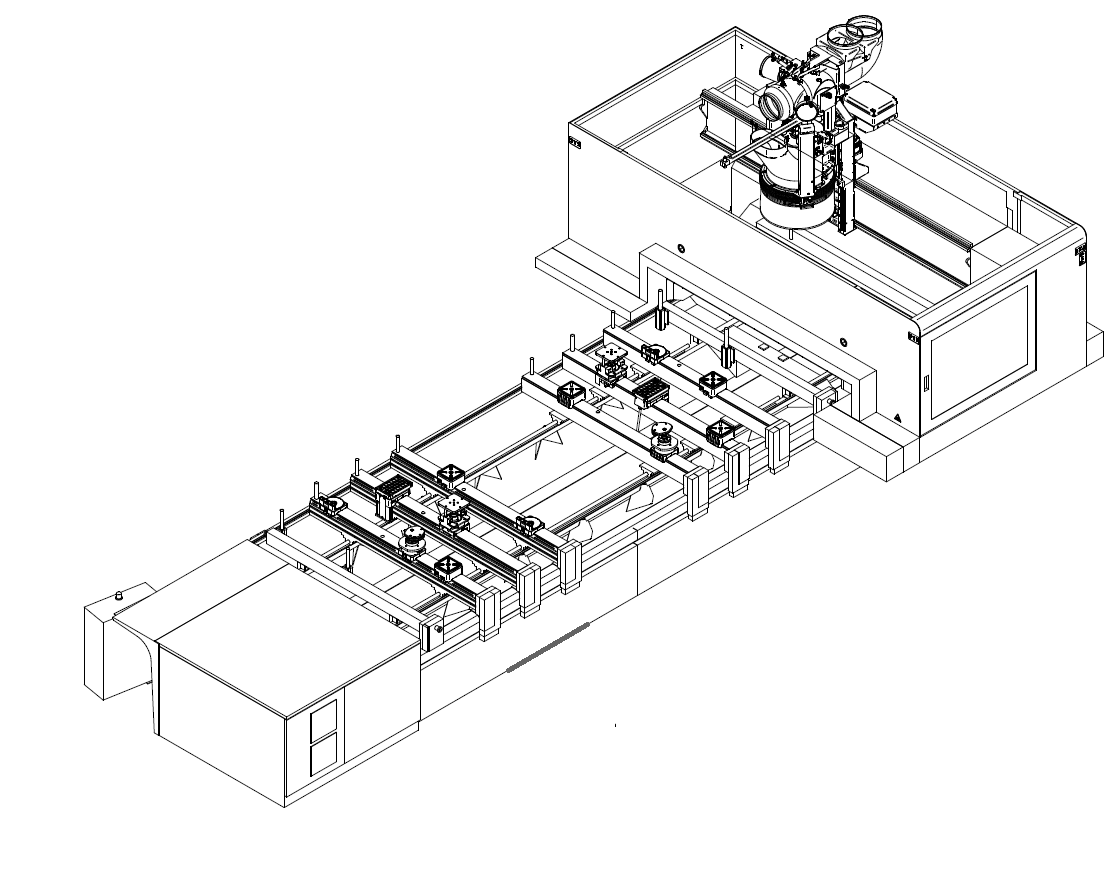
\includegraphics[width=\textwidth]{figures/worktable.png}
		\caption{Work center}
		\label{fig:worktable}
	\end{subfigure}
	\hspace{2cm}
	\begin{subfigure}[b]{0.4\textwidth}
		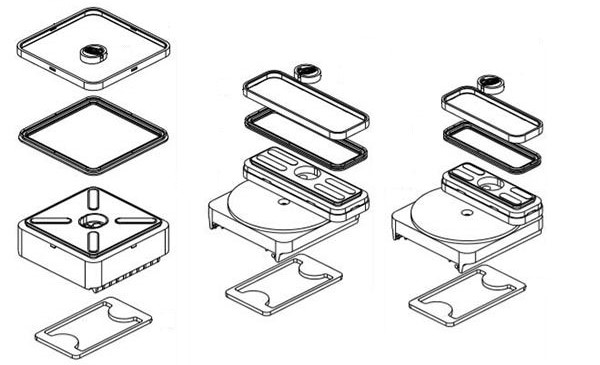
\includegraphics[width=\textwidth]{figures/suction_cups_schema_no_dimnesion.jpg}
		\caption{Vacuum suction cup fixtures}
		\label{fig:suction_cups}
	\end{subfigure}
	\caption{On the left, a work center featuring a worktable with movable bars. On the right, fixtures used to secure the workpiece during machining operations.}
	\label{fig:problem_description_img}
\end{figure}

Determining an appropriate fixture layout for a given workpiece is not always straightforward for a human operator, especially when the workpiece has contoured shapes or includes areas to be extruded. Layouts are often based on the operator’s experience; however, such manually designed solutions are not necessarily optimal and can often be improved by considering the structural properties of the fixtures system, such as its resistance to bending and torsional forces.

The purpose of this work is to determine a sound, and possibly optimal, placement of fixtures under the bottom surface of the workpiece, explicitly accounting for the rotation angle of each fixture.

To solve the problem, we first consider a simplified version that neglects fixture rotation and extrusion areas, addressing it through the formulation of a solver-independent Constraint Programming (CP) model. The performance of the model were evaluated using different solvers and two alternative objective functions: one based on the exact computation of the principal moments of inertia, and the other based on the Manhattan distance between pairs of fixtures.

According to the results obtained and considering more real-world test instances, we revisited the objective function and extended the CP formulation to account for extrusion areas. The performance of the extended CP model were then compared with other solution strategies based on a newly formulated Mixed Integer Programming (MIP) model and a Q-learning based algorithm.

The CP model, the MIP model, and the Q-learning algorithm do not consider fixture rotations, as allowing arbitrary rotation angles significantly increases the number of possible configurations and makes the problem substantially harder to solve. Rotations are subsequently incorporated through a refinement stage based on the Particle Swarm Optimization (PSO) meta-heuristic initialized from the layouts obtained from CP, MIP and Q-learning.

This first part of the thesis is organized as follows. Chapter~\ref{chap:pt1_state_of_the_art} reviews the state of the art. Chapter~\ref{chap:pt1_chapter5} introduces the simplified problem formulation and presents the CP model used to solve it. Chapter~\ref{chap:pt1_chapter6} addresses the complete problem by considering fixture rotations and extrusion areas. Chapter~\ref{chap:pt1_chapter7} analyzes the integration of the proposed solution strategies. Finally, Chapter~\ref{chap:pt1_conclusion} concludes this part of the thesis.

	
	\chapter{State of the art}
	\label{chap:pt1_state_of_the_art}

The problem of determining a fixture layout that maximizes workpiece stability has been widely studied in the literature. One class of approaches formulates fixture layout as a mathematical optimization problem, often coupled with Finite Element Analysis (FEA)~\cite{bhavikatti2005finite} to evaluate workpiece deformation. Menassa and DeVries~\cite{menassa1991optimization} proposed the use of the Broyden--Fletcher--Goldfarb--Shanno (BFGS) optimization algorithm to determine fixture support locations that minimize deformation. This direction was further explored by Cai et al.~\cite{cai1996deformable}, who combined nonlinear programming with FEA to optimize fixture layouts under a given force, while Camelio et al.~\cite{camelio2004impact} later extended the same approach to minimize shape variations in assembled products. Li and Melkote~\cite{li2001optimal} applied Sequential Quadratic Programming (SQP) to jointly optimize fixture layout and clamping forces. Subsequently, Li et al.~\cite{li2010variation} proposed a flexible fixture system for sheet metal assembly based on assembly variation analysis using the Lagrangian conditional extremum method, while Zhang et al.~\cite{zhang2010fixture} developed a nonlinear optimization model solved using the Augmented Lagrangian method.

Evolutionary and meta-heuristic optimization techniques have also been widely investigated. Kulankara et al.~\cite{kulankara2002iterative} proposed a Genetic Algorithm (GA) for the simultaneous optimization of fixture positions and clamping forces. Shortly afterwards, Y.~Gene Liao~\cite{liao2003genetic} introduced a two-phase GA to identify and refine locating and clamping zones in sheet-metal assembly. Padmanaban et al.~\cite{padmanaban2009machining} combined FEA with discrete and continuous Ant Colony Algorithms (ACA) to reduce sheet metal deformation. Sundararaman et al.~\cite{sundararaman2016optimization} proposed a fixture layout optimization approach combining Response Surface Methodology (RSM), Genetic Algorithms (GA), and Particle Swarm Optimization (PSO), reporting superior performance with PSO. More recently, Liu et al.~\cite{liu2024fixture} introduced an Improved Particle Swarm Optimization (IPSO) algorithm for the fixture layout optimization of large thin-walled parts.

Learning-based methods have recently emerged as an alternative strategy. Selvakumar et al.~\cite{selvakumar2013design} combined Artificial Neural Networks (ANNs) with Design of Experiments (DOE) for machining fixture layout optimization. Wang et al.~\cite{wang2016optimal} integrated neural networks with the Bat Algorithm (BA) to minimize workpiece deformation. Low et al.~\cite{low2020study} proposed a Reinforcement Learning (RL) framework for fixture design, while Wang et al.~\cite{wang2025smartfixture} presented a physics-guided RL approach in which the agent is trained through interaction with an FEA-based simulation.

\begin{figure}[t]
	\centering
	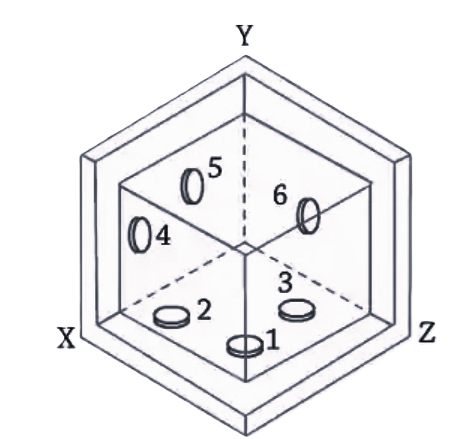
\includegraphics[width=0.35\textwidth]{figures/locating_principle.png}
	\caption{Example of the application of the ``3-2-1'' locating principle for the stabilization of a workpiece}
	\label{fig:locating_principle}
\end{figure}

Although numerous studies on fixture layout optimization exist in the literature, few focus on suction cup fixtures with characteristics similar to those used in wood industry. Most existing research has been conducted in the \emph{metal industry}, where the objective is to determine the number and placement of fixtures according to the ``$N$-2-1'' locating principle in order to minimize workpiece deformation. The ``$N$-2-1'' principle is a generalization of the classical ``3-2-1'' locating scheme. In the latter, three locators constrain the primary datum plane, two constrain the secondary datum, and one constrains the tertiary datum, thereby fully restricting the six rigid-body degrees of freedom of the workpiece, as shown in Figure~\ref{fig:locating_principle}. The ``$N$-2-1'' principle replaces the three primary locators with $N$ locators, while retaining two and one locators on the secondary and tertiary datum planes~\cite{wang2016optimal}.

However, this principle cannot be directly applied to work centers in the wood industry, where the workpiece can only be supported from below. Furthermore, the fixtures adopted in the metal industry generally differ from those used in wood industry, as they typically do not allow rotation. While allowing fixture rotation can significantly improve workpiece stability, it also substantially increases the number of possible solutions and therefore the complexity of the optimization problem.

	
	\chapter{Simplified problem formulation}
	\label{chap:pt1_chapter5}
The original problem consists of determining, given the workpiece geometry, the available fixtures (possibly of different sizes), and the available worktable bars, a set of fixtures together with their positions, orientations, and types that maximize workpiece stability.

We first consider a simplified version of the problem, assuming that the workpiece does not contain areas to be extruded and neglecting fixture rotations. Under these assumptions, to ensure the feasibility of a layout the following constraints must be satisfied:
\begin{enumerate}
	\item the number of placed fixtures must not exceed their availability;
	\item fixtures must be positioned so as to satisfy the minimum safety distances;
	\item fixtures must lie within the boundaries of the workpiece and beneath its surface;
	\item fixtures must not overlap each other.
\end{enumerate}

We address this problem by proposing a CP model implemented in the MiniZinc language~\cite{nethercote2007minizinc}. The model is parametric with respect to the input data and solver-independent. Consequently, it can be solved using any solver that support MiniZinc, not only CP-based solver, but also alternatives such as Mixed-Integer Programming (MIP) and Constraint Logic Programming (CLP) solvers.

\section{Model formulation}
\label{sec:first_cp_model}
In this section we describe the CP model in terms of input parameters, variables, constraints, and objective function(s). 
The model is \emph{parametric} because it is defined in terms of its parameters: changing the input data does not affect the model itself.

\subsection{Parameters}
\label{sec:first_parameters}
The input parameters shaping a particular problem instance are:

\begin{itemize}
	\item the width $\wtab$ and height $\htab$ of the machine worktable;
	\item the minimum horizontal distance $\wmin$ between two fixtures placed on different bars;
	\item the number $\ntypes$ of different fixture types;
	\item the number $\nfix_i$ of available fixtures for each type $i \in [1..\ntypes]$;
	\item the total number of available fixtures $\nfix = \sum_{i=1}^{\ntypes} \nfix_i$;
	\item the minimum $\nmin$ and maximum $\nmax$ number of fixtures to place;
	\item the width $\wfix_i$ and height $\hfix_i$ of each fixture of type $i$;
	\item the workpiece shape, defined by a set of linear inequalities of the form $\mathtt{a}x + \mathtt{b}y + \mathtt{c} \leq 0$;
\end{itemize}

\subsection{Variables}
\label{sec:first_variables}
To determine which fixtures to use and their positions on the worktable, we define three arrays of variables $x$, $y$, $t$ of size $\nfix$ such that, for $i = 1,\dots,\nfix$:
\begin{itemize}
	\item \( (x_i,y_i) \) is the coordinate of the lower-left corner of the $i$-th fixture,  with \( x_i \in [0..\wtab] \) and \( y_i \in [0..\htab] \)
	\item $t_i$ is the type of the $i$-th fixture, with \( t_i \in [0..\ntypes] \)
\end{itemize}
We also define a variable $n_i \in [0..\nfix_{t_i}]$ for each  \(i \in [0..\ntypes] \) counting the number of fixtures of type $i$, and a variable $n$ 
corresponding to the total number of fixtures employed.

\subsection{Constraints}
\label{sec:first_constraints}
For each fixture of type $i \in [1..\ntypes]$, we impose the CP \emph{global} constraint~\cite{DBLP:journals/constraints/BeldiceanuCDP07}: $$n_i = \mathtt{count}(t,i)$$ counting the number of fixtures in $t$ with type $i$, and set $n = \sum_i n_i$.

To break symmetries that arise when fixtures of the same type are permuted without
changing their spatial arrangement, we impose a lexicographic ordering such that $(x_{i-1},y_{i-1}) \preceq (x_i,y_i)$ for $i \in [2..\nfix{}]$ through the $\mathtt{lex\_chain}$ global constraint. 

Because we may not use all the available fixtures,
we enforce the invariant: $$ (i > n) \iff (x_i = \wtab ~\wedge~ y_i = \htab ~\wedge~ t_i = 0)$$


The workpiece region is defined by a set of linear inequalities of the form $\mathtt{a}x + \mathtt{b}y + \mathtt{c} \leq 0$. Therefore, to ensure that the fixtures lie within the workpiece boundaries, each fixture coordinate $(x_i, y_i)$, for $i \leq n$, must satisfy the condition 
$\mathtt{a}x' + \mathtt{b}y' + \mathtt{c} \leq 0$ where:

\[
x'_i = 
\begin{cases}
	x_i & \text{if }a \leq 0\\
	x_i + \wfix_{t_i} & \text{if }a > 0
\end{cases}
\qquad
y'_i = 
\begin{cases}
	y_i & \text{if }b \leq 0\\
	y_i + \hfix_{t_i} & \text{if }b > 0
\end{cases}
\]

Indeed, according to the sign of coefficients $\mathtt{a}$ and $\mathtt{b}$, we only have to check that one vertex of the rectangular fixture is within the workpiece region. 
For example, if the inequality is $3x - 2y + 4 \leq 0$, we impose $3(x_i + \wfix_{t_i}) - 2y_i + 4 \leq 0$ to enforce the lower-right corner within the hyperplane 
defined by that inequality. If so, also all the other fixture points must be within that region, as shown in Figure~\ref{fig:geometricconstraint}.

\begin{figure}[t]
	\centering
	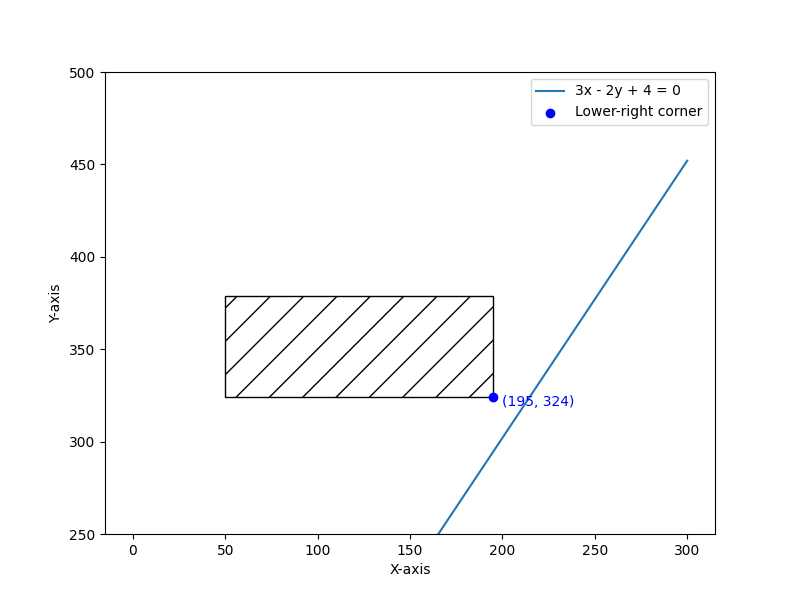
\includegraphics[width=0.5\linewidth]{figures/geometry_constraint.png}
	\caption{Geometric constraint for fixtures placement}
	\label{fig:geometricconstraint}
\end{figure}

To encode the no-overlap constraint between fixtures we employ the $\mathtt{diffn}$ global constraint~\cite{DBLP:journals/constraints/BeldiceanuCDP07}:
\begin{align*}
	\mathtt{diffn}(x, y, [\wfix_{t_i} \mid i \in [1..n]], [\hfix_{t_i} \mid i \in [1..n] ])
\end{align*}

This constraint ensures that each rectangle with origin in the lower-left corener $(x_i,y_i)$, width $\wfix_{t_i}$ and height $\hfix_{t_i}$ is not overlapping. Specifically, we use the \emph{non-strict} version of $\mathtt{diffn}$, in which zero-width rectangles can be positioned anywhere, ignoring the $\nfix{} - n$ unemployed fixtures.

The same constraint can be naturally extended to prevent fixtures from being placed within areas to be extruded, as will be described in Section~\ref{sec:second_cp_cons}.

Finally, we guarantee that the horizontal distance between two fixtures placed on different bars is at least $\wmin$. Formally, for each $i \in [1..n-1]$ we impose that:
$$x_{i} \neq x_{i+1} \implies x_{i} + \wfix_{t_{i}} + \wmin \leq x_{i+1}$$

\subsection{Objective function}
\label{sec:first_objective_function}
As illustrated in Chapter~\ref{chap:pt1_background}, is possible to maximize workpiece stability by maximizing the principal moments of inertia. Consequently, the ideal objective function would be: 

\begin{equation}
	\finer = J_\xi + J_\eta
	\label{eq:f_iner}
\end{equation}
where $J_\xi$ and $J_\eta$ are the principal moments of inertia defined in Section~\ref{sec:principal_moment_of_inertia}.

However, computing $J_\xi$ and $J_\eta$ involves nonlinear operations such as squaring, square roots, and transcendental functions (sine and cosine), which are difficult to handle efficiently with CP solvers~\cite{leyffer2009applications}.

An analysis of the moment of inertia for different fixture layouts, together with previous studies on workpiece stability~\cite{kaya2006machining,roy1999geometric,menassa1991optimization,meyer1997fixture,wallack1997planning}, indicates that workpiece stability increases when fixtures are placed far apart from one another and close to the workpiece perimeter. Based on these observations, we devised an alternative objective function, $\fdistsemi$, that maximizes the sum of the pairwise Manhattan distances between fixture centroids, augmented by the semi-perimeter of the selected fixtures.

\begin{equation}
	\fdistsemi = \sum_{1 \le i < j \le n} \left(|cx_i - cx_j| + |cy_i - cy_j|\right) + \sum_{k=1}^{n} (\wfix_{t_k} + \hfix_{t_k})
	\label{eq:f_dist_semi}
\end{equation}
\noindent where $(cx_i,cy_i) = (x_i + \frac{\wfix_{t_i}}{2}, y_i + \frac{\hfix_{t_i}}{2})$
are the coordinates of the centroid of the $i$-th placed fixture, having type $t_i$.

\section{Case study}
\label{sec:case_study}
We evaluated our approach on a real case where the workpiece is a stair step of a spiral staircase. The workpiece area, shown in Figure.~\ref{fig:stairstepworkpiece}, is defined by the following inequalities:
\begin{align*}
	(a):~ x &\geq 20 & (d):~ x &\leq 689\\
	(b):~ y &\leq 0.20x + 257.91 & (e):~ y &\geq 0.54x + -356.21\\
	(c):~ y &\leq -0.58x + 781.92 &  (f):~ y &\geq -0.20x + 139.06
\end{align*}

\begin{figure}[t]
	\centering  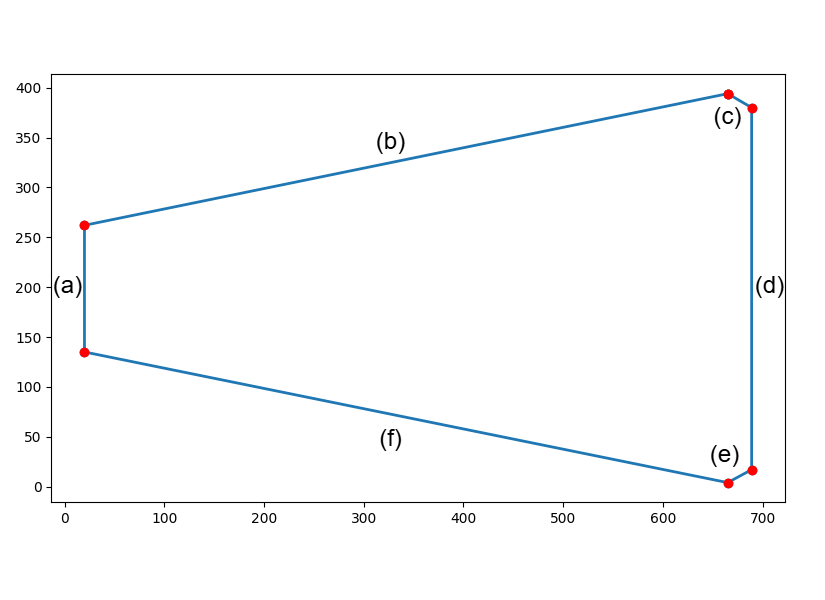
\includegraphics[width=0.5\linewidth]{figures/stair_step_line_equations.png}
	\caption{Stair step of a spiral staircase}
	\caption{A polygonal workpiece representing a stair step}
	\label{fig:stairstepworkpiece}
\end{figure}

The width and height of the worktable are respectively $\wtab = 700$ and $\htab = 400$.
The minimal horizontal distance between fixtures is $\wmin = 140$.
We have two different types of fixtures available:
\begin{itemize}
	\item five square fixtures of dimension \(145 \times 145 \text{ mm}\);
	\item five rectangular fixtures of dimension \(145 \times 55 \text{ mm}\).
\end{itemize}
So, $\nfix_{1} = \nfix_{2} = 5$ with $\wfix_{1} = \hfix_{1} = \wfix_{2} = 145$ and $\hfix_{2}=55$.

We set an upper bound $\nmax$ on the number of fixtures (i.e., we impose $n\leq\nmax$) and we evaluated different values of $\nmax$ in the range $[2..10]$.
We assume a minimum number of 2 fixtures (i.e., $n \geq 2$) as placing only one fixture is not a realistic case.

We defined two models, one using the objective function $\finer$ and the other using $\fdistsemi$. Both were implemented in Minizinc~\cite{nethercote2007minizinc}. For the model using $\fdistsemi$, four solvers were evaluated: Chuffed~\cite{chuffed}, Gecode~\cite{schulte2006gecode}, OR-Tools~\cite{ortools} and Gurobi~\cite{gurobi}. For the $\finer$ model, we restricted our evaluation to solvers that support floating-point variables, namely Gecode and Gurobi.

All experiments were conducted with a time limit of 300 seconds on a 64-bit Windows machine equipped with an Intel Core i5 CPU and 16 GB of RAM. 

Table~\ref{tab:solvercomparison_momentobj} and Table~\ref{tab:solvercomparison_distobj} report the results obtained using $\finer$ and $\fdistsemi$ as objective functions, respectively, across different values of $\nmax$. Specifically, Table~\ref{tab:solvercomparison_distobj} doesn't report the value of $\fdistsemi$ but the corresponding \emph{a posteriori} values of $\finer$ for the best solutions found by the solvers.

In Table~\ref{tab:solvercomparison_momentobj} the result for the Gecode solver are not reported, as it fails to find any feasible solution within the time limit. On the other hand, Gurobi being a MIP solver that handle continuous variables, is able to find optimal solutions for $\nmax \leq 5$ but is not able to find any solution for $\nmax \geq 6$. 

When using $\fdistsemi$ as the objective function, Table~\ref{tab:solvercomparison_distobj} shows that all solvers are able to find at least one feasible solution for every value of $\nmax$, with Chuffed and Gurobi solving all instances to optimality. Overall, the best performance is achieved by Chuffed, which is able to reach the optimal solutions in less time than Gurobi.

In the tables the optimal solutions found are reported in bold, the $\fdistsemi$ objective function can admit multiple equivalent optimal solutions; however, these solutions may lead to different values of $\finer$, due to the high sensitivity of the moments of inertia to small fixture displacements, as reported for $\nmax \in {3,4,5}$ in Table~\ref{tab:solvercomparison_distobj}.

Comparing the two tables, we can observe that solutions generated using $\fdistsemi$ generally achieve lower $\finer$ values, but can be computed significantly faster, making this objective function particularly suitable for large workpieces or instances requiring a high number of fixtures. Indeed, comparing the runtimes obtained by Gurobi with the two objective functions shows that solving the problem with $\fdistsemi$ is on average more than 150 times faster than using $\finer$.

\begin{landscape}
	
	\begin{table}[p]
		\centering
		\small
		\caption{Results for $\finer$. All $\finer$ values reported in units of $10^9$. Bold fold indicates the best $\finer$ value found before the timeout.}
		\label{tab:solvercomparison_momentobj}
		\renewcommand{\arraystretch}{1.2}
		
		\begin{tabular}{p{1.5cm}p{1.5cm}ccccccccc}
			\toprule
			\multicolumn{2}{c}{} & \multicolumn{9}{c}{$\nmax$} \\
			\cmidrule(lr){3-11}
			\textbf{Solver} & \textbf{Metric} & 2 & 3 & 4 & 5 & 6 & 7 & 8 & 9 & 10 \\
			\midrule
			Gurobi & Runtime [ms]
			& 14250 & 189000 & 90000 & 258000 & -- & -- & -- & -- & -- \\
			& $\finer$
			& \textbf{2.65072}
			& \textbf{3.79990}
			& \textbf{3.79990}
			& \textbf{3.87506}
			& 3.89034
			& --
			& --
			& --
			& -- \\
			\bottomrule
		\end{tabular}
	\end{table}
	
\end{landscape}

\begin{landscape}
	
	\begin{table}[p]
		\centering
		\small
		\caption{Results using $\fdistsemi$. Bold fold denotes the $\finer$, reported in units of $10^9$, corresponding to a $\fdistsemi$-optimal solution.}
		\label{tab:solvercomparison_distobj}
		\renewcommand{\arraystretch}{1.0}
		
		\begin{tabular}{p{1.5cm}p{1.5cm}ccccccccc}
			\toprule
			\multicolumn{2}{c}{} & \multicolumn{9}{c}{$\nmax$} \\
			\cmidrule(lr){3-11}
			\textbf{Solver} & \textbf{Metric} & 2 & 3 & 4 & 5 & 6 & 7 & 8 & 9 & 10 \\
			\midrule
			
			Chuffed & Runtime [ms]
			& 1566 & 904 & 2039 & 3333 & 3700 & 2533 & 4873 & 5222 & 5593 \\
			& $\finer$
			& \textbf{2.64416}
			& \textbf{2.38480}
			& \textbf{2.58584}
			& \textbf{3.54968}
			& \textbf{3.80905}
			& \textbf{3.80905}
			& \textbf{3.80905}
			& \textbf{3.80905}
			& \textbf{3.80905} \\
			\midrule
			
			Gurobi & Runtime [ms]
			& 503 & 745 & 961 & 1098 & 1540 & 1856 & 4674 & 5534 & 10840 \\
			& $\finer$
			& \textbf{2.64416}
			& \textbf{2.38350}
			& \textbf{2.58584}
			& \textbf{3.08459}
			& \textbf{3.80905}
			& \textbf{3.80905}
			& \textbf{3.80905}
			& \textbf{3.80905}
			& \textbf{3.80905} \\
			\midrule
			
			Gecode & Runtime [ms]
			& 549 & 18292 & -- & -- & -- & -- & -- & -- & -- \\
			& $\finer$
			& \textbf{2.64416}
			& \textbf{2.39170}
			& 2.58584
			& 2.58584
			& 2.58584
			& 3.73308
			& 2.58584
			& 2.58584
			& 2.58584 \\
			\midrule
			
			OR-Tools & Runtime [ms]
			& 882 & 7804 & 260000 & -- & -- & -- & -- & -- & -- \\
			& $\finer$
			& \textbf{2.64416}
			& \textbf{2.16912}
			& \textbf{2.24606}
			& \textbf{3.34565}
			& 3.34565
			& 3.38321
			& 3.73467
			& 3.73467
			& 3.67863 \\
			\bottomrule
		\end{tabular}
		
	\end{table}
	
\end{landscape}

Tables~\ref{tab:visual_results_234_fdist} and~\ref{tab:visual_results_5_10_fdist} present the visual results obtained from the different solvers using the $\fdistsemi$ objective function, evaluated across varying values of $\nmax$, while Tables~\ref{tab:visual_results_234_finer} and~\ref{tab:visual_results_5_10_finer} report the corresponding layouts obtained with Gurobi when optimizing $\finer$.

The layouts obtained with $\fdistsemi$ are generally similar across solvers. However, when the number of fixtures is limited to three, Chuffed, Gecode, and OR-Tools tend to place a smaller fixture on the left side of the workpiece, below its center, whereas Gurobi positions the smaller fixture closer to the center and places two larger fixtures on the right side, leading to a higher $\finer$ value, as reported in Table~\ref{tab:solvercomparison_distobj}.

As expected, optimizing $\finer$ promotes the selection of larger fixtures, since larger support areas result in higher moments of inertia. For instance, with three fixtures, the solution provided by Gurobi using the $\finer$ objective function selects only the largest available fixtures. This configuration is maintained also for $\nmax=4$, where the solver avoids introducing an additional fixture.


\begin{landscape}
	
	% =====================================================
	% TABLE 1: n = 2–4 (all solvers EXCEPT Gurobi f_iner)
	% =====================================================
	\begin{table}[p]
		\centering
		\small
		\caption{Visual results for solvers’ solutions using $\fdistsemi$ as objective function ($\nmax = 2$--$4$).}
		\label{tab:visual_results_234_fdist}
		\renewcommand{\arraystretch}{1.5}
		
		\begin{tabular}{lccc}
			\toprule
			\multicolumn{1}{c}{} & \multicolumn{3}{c}{$\nmax$} \\
			\cmidrule(lr){2-4}
			\textbf{Solver} & 2 & 3 & 4 \\
			\midrule
			
			\raisebox{+6.0\height}{Chuffed} &
			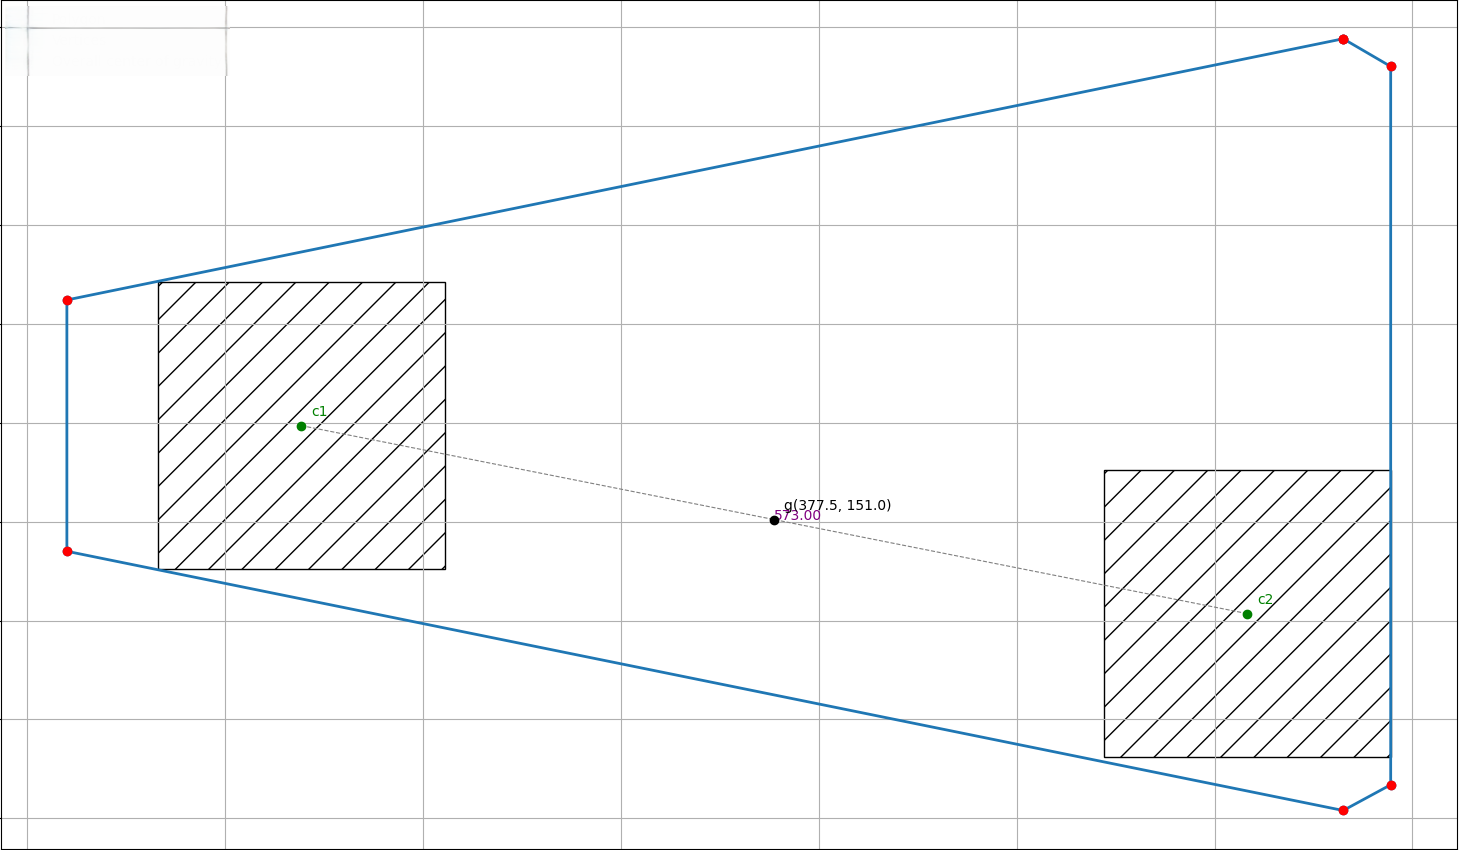
\includegraphics[width=1.8in]{figures/chuffed2.png} &
			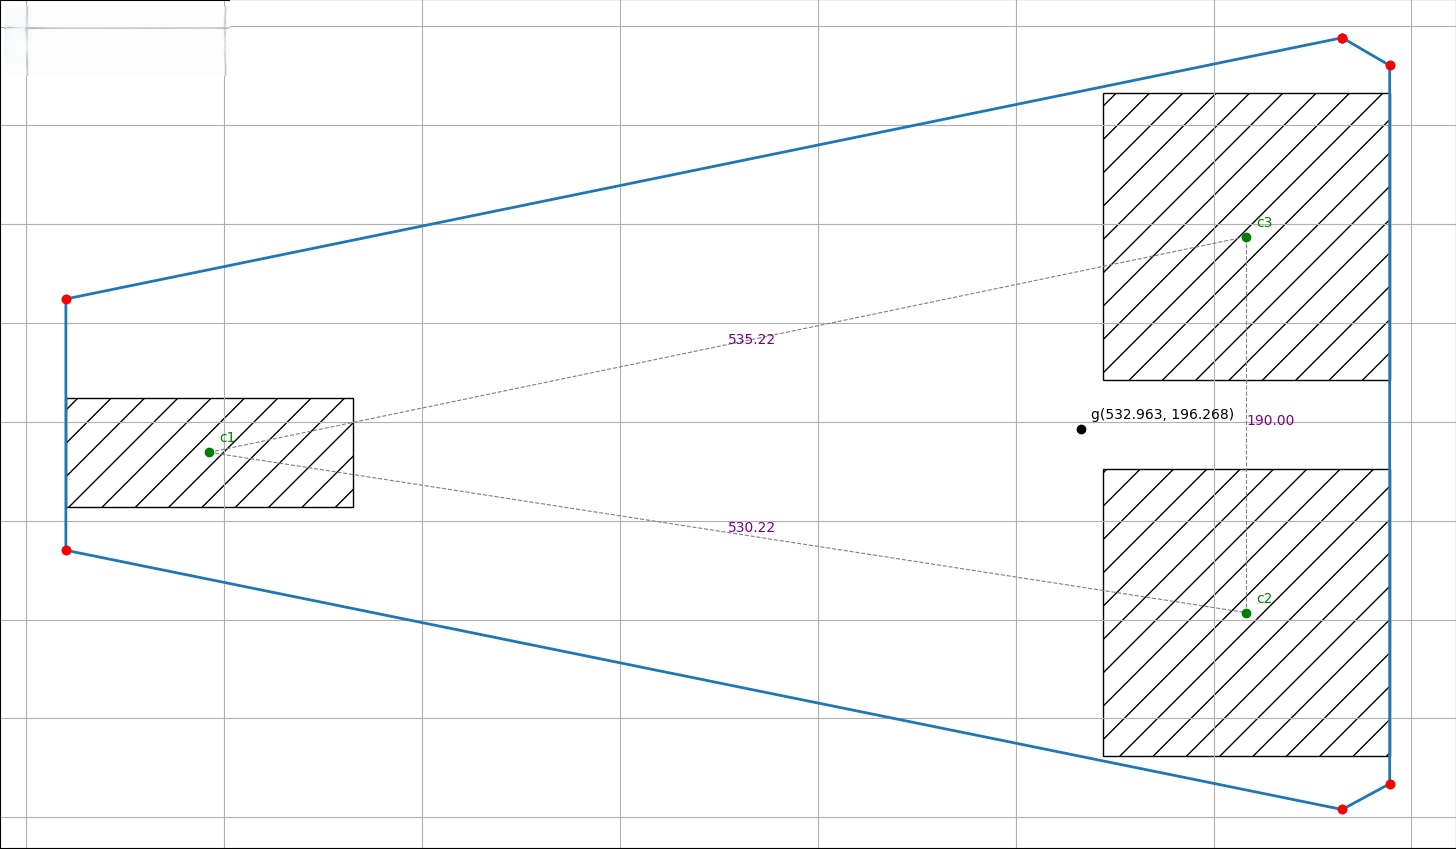
\includegraphics[width=1.8in]{figures/chuffed3.png} &
			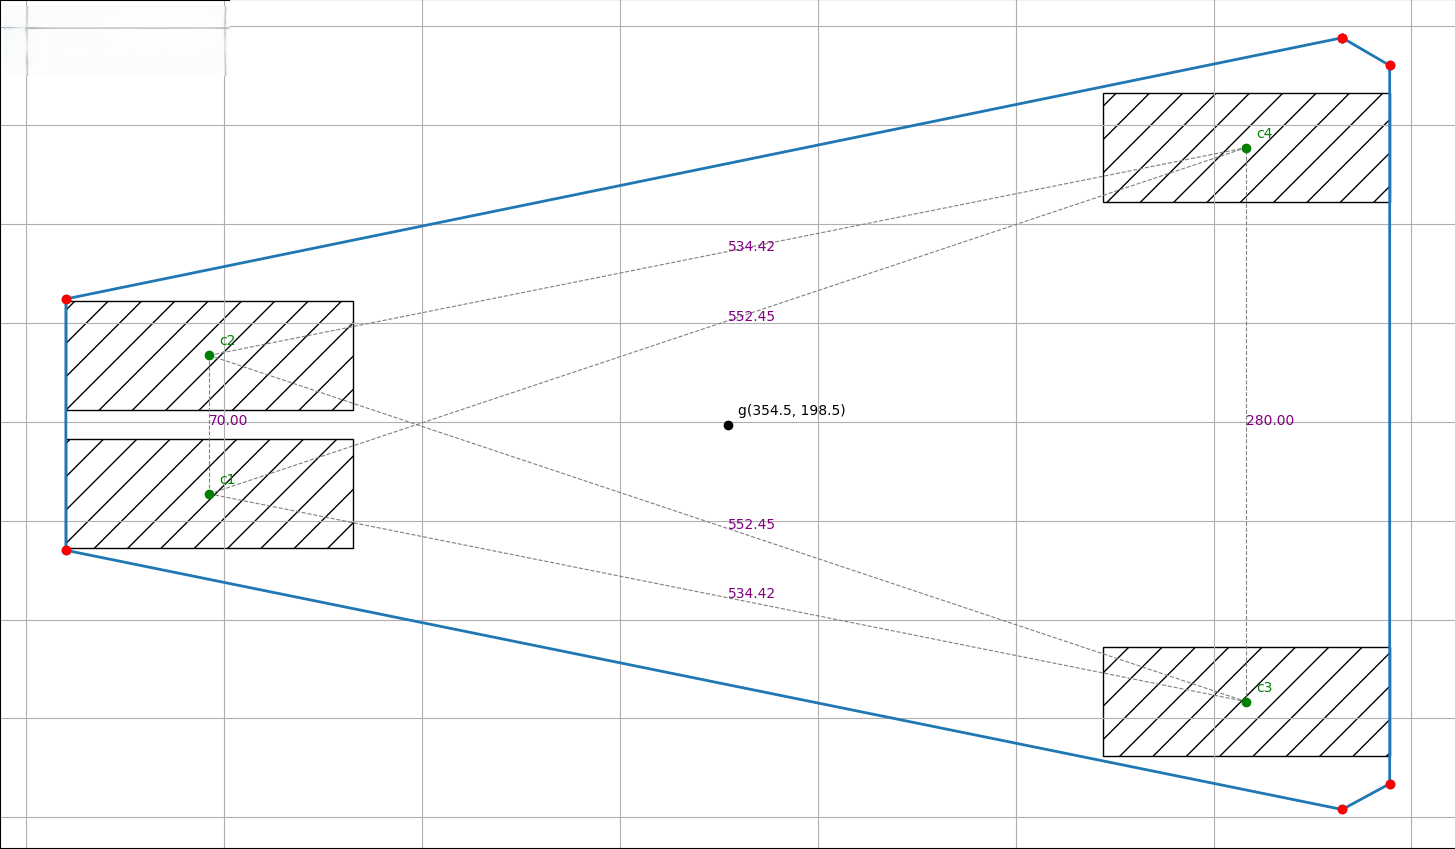
\includegraphics[width=1.8in]{figures/chuffed4.png} \\
			
			\raisebox{+6.0\height}{Gecode ($\fdistsemi$)} &
			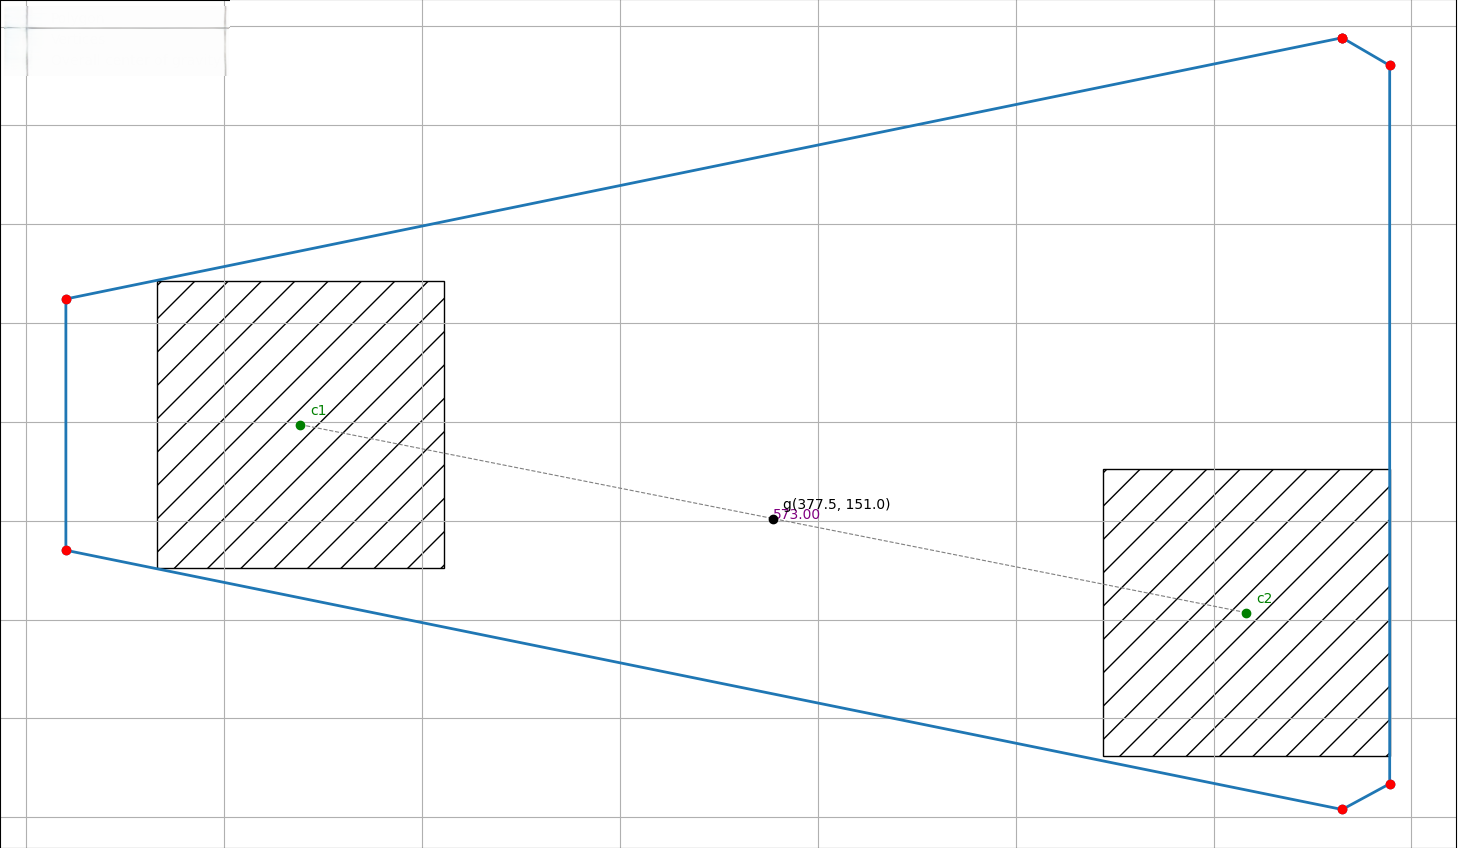
\includegraphics[width=1.8in]{figures/gecode2.png} &
			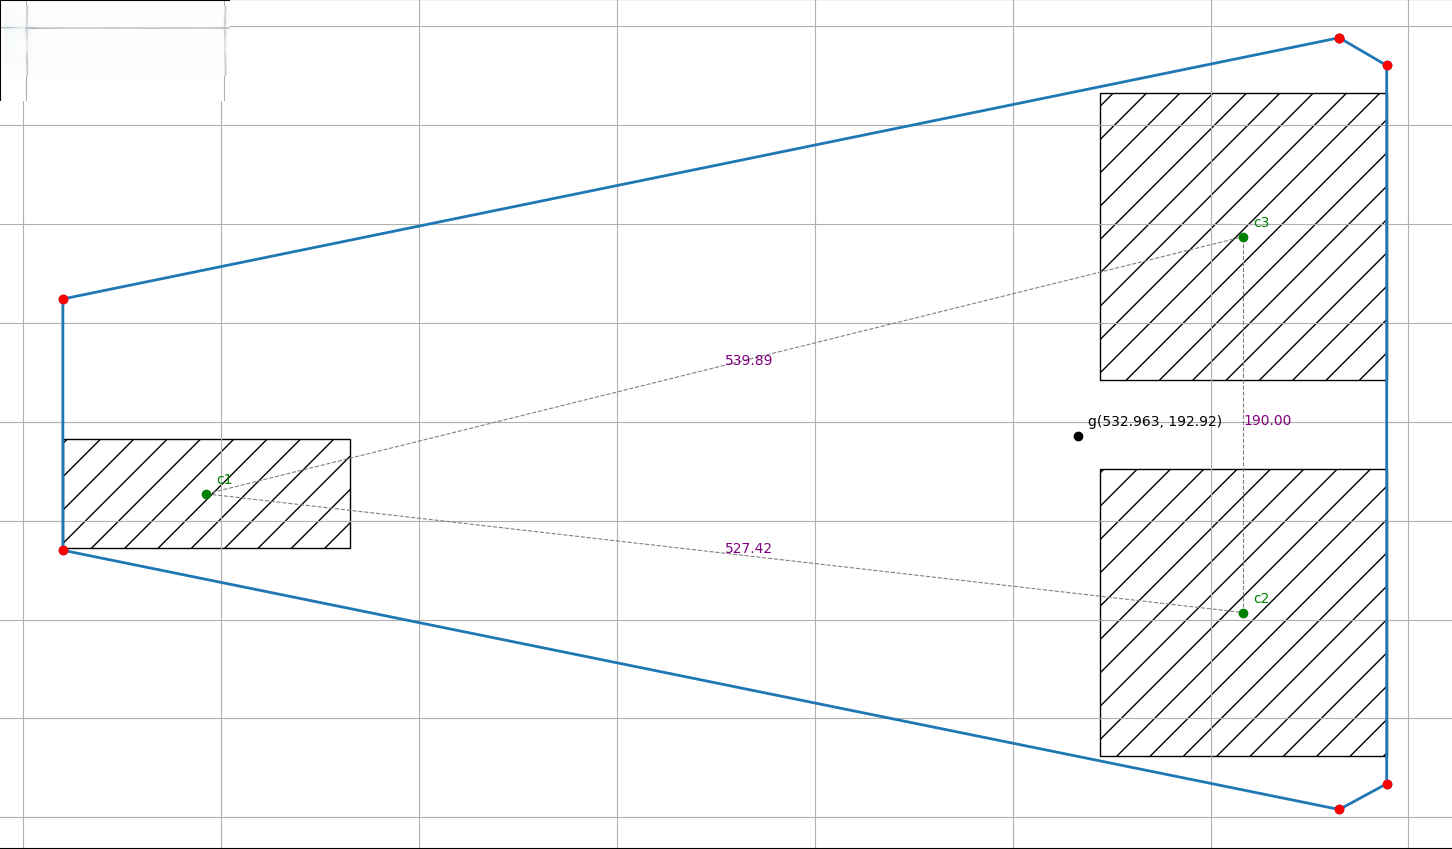
\includegraphics[width=1.8in]{figures/gecode3.png} &
			\raisebox{+12.0\height}{--} \\
			
			\raisebox{+6.0\height}{OR-Tools} &
			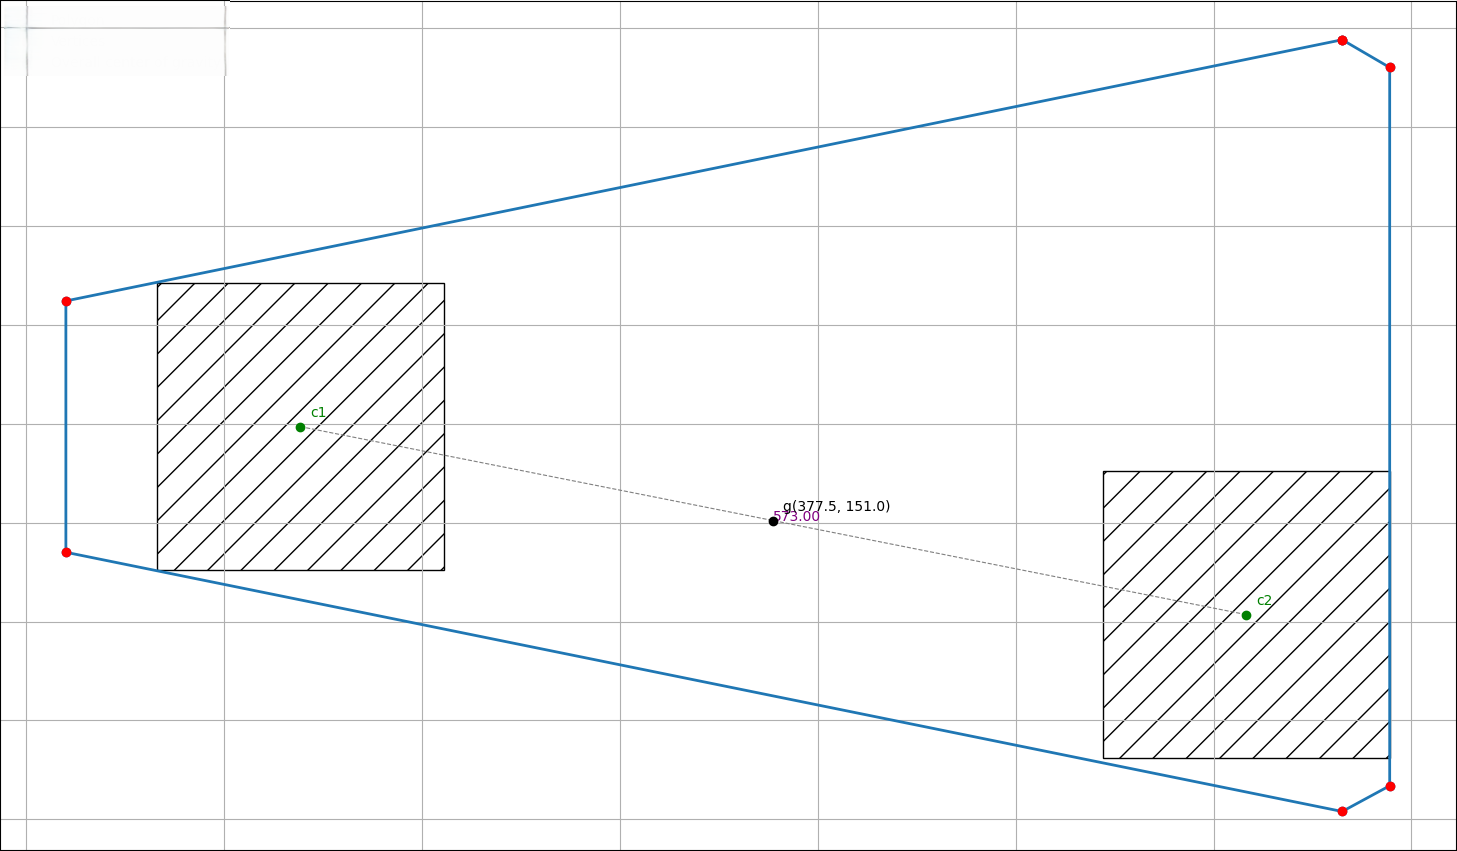
\includegraphics[width=1.8in]{figures/ortools2.png} &
			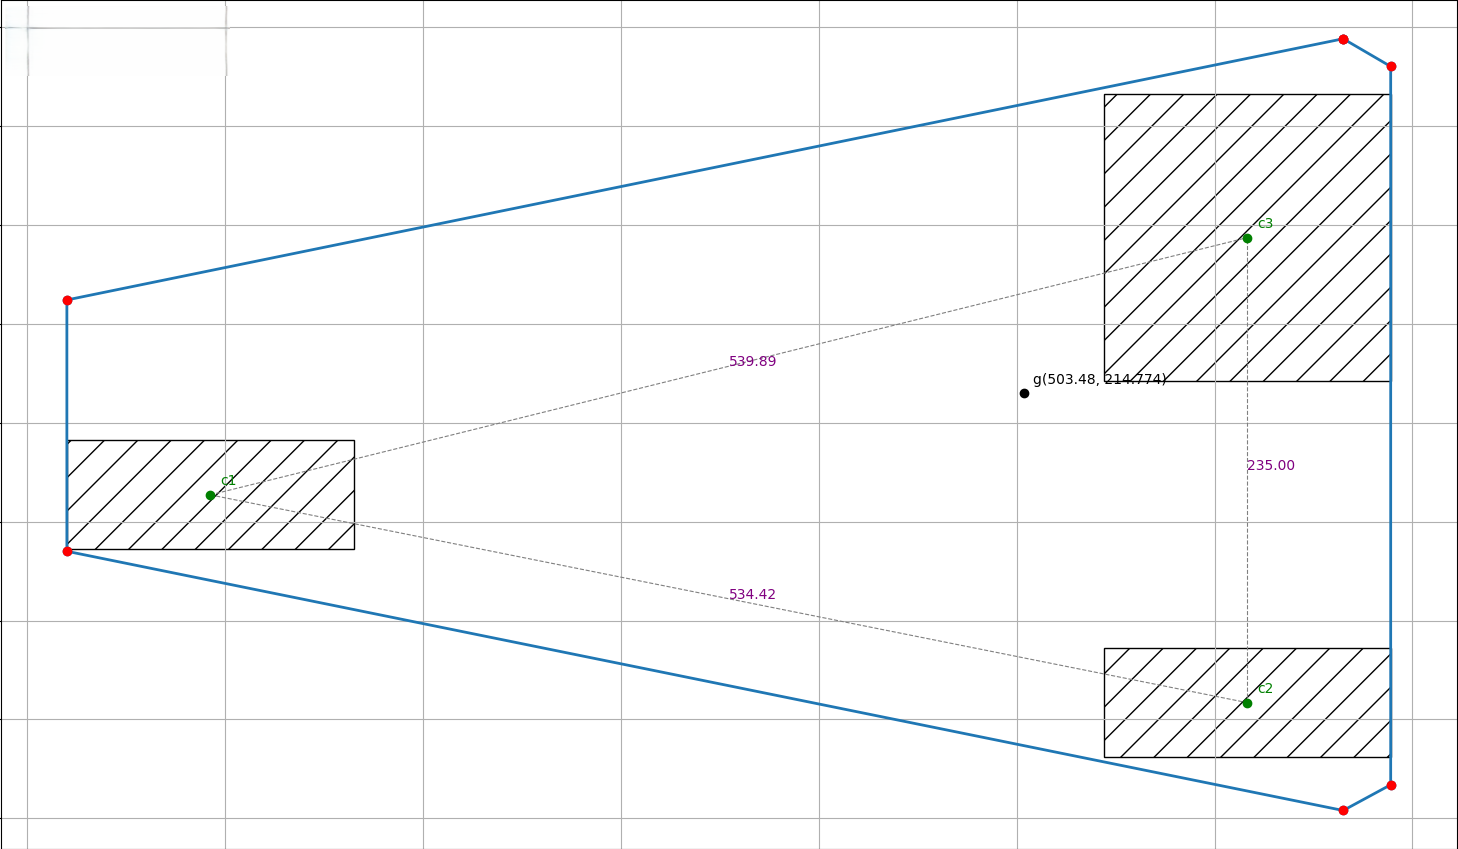
\includegraphics[width=1.8in]{figures/ortools3.png} &
			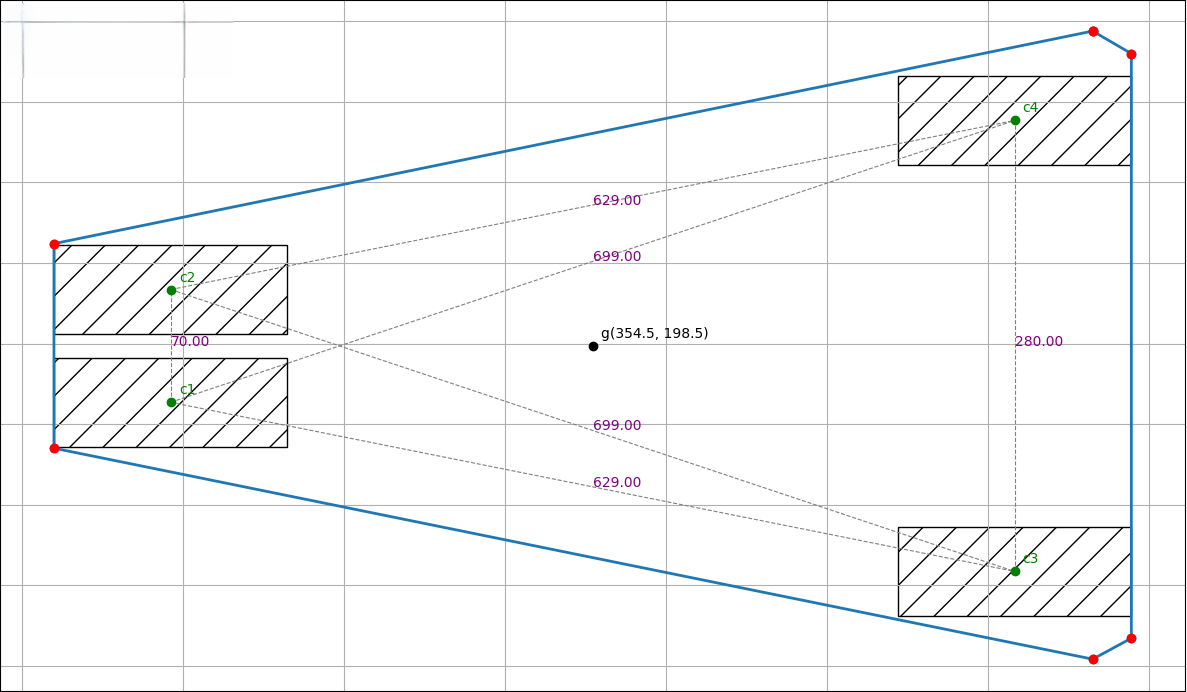
\includegraphics[width=1.8in]{figures/ortools4.png} \\
			
			\raisebox{+6.0\height}{Gurobi ($\fdistsemi$)} &
			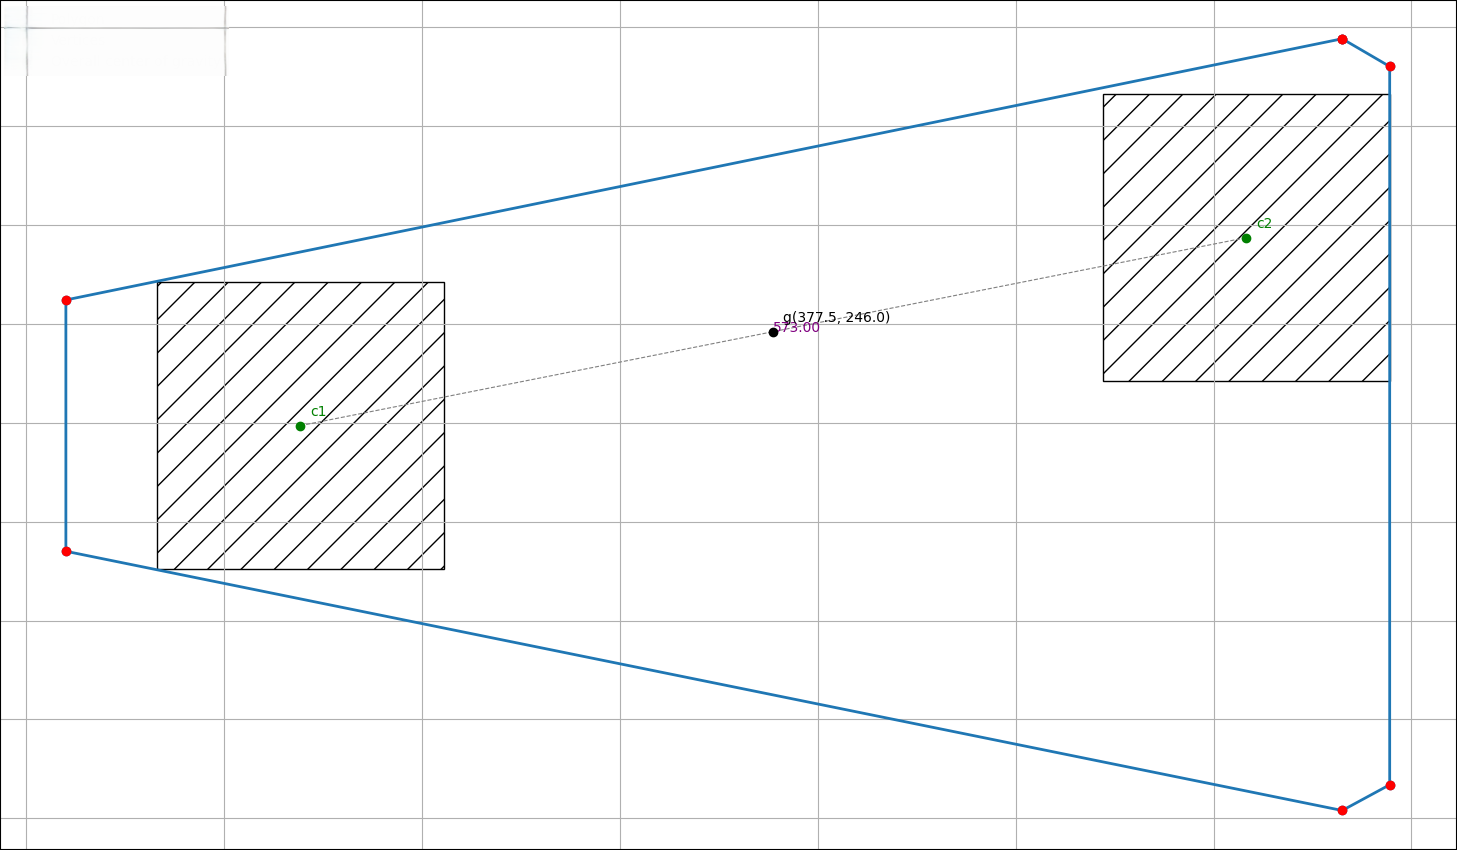
\includegraphics[width=1.8in]{figures/gurobi2.png} &
			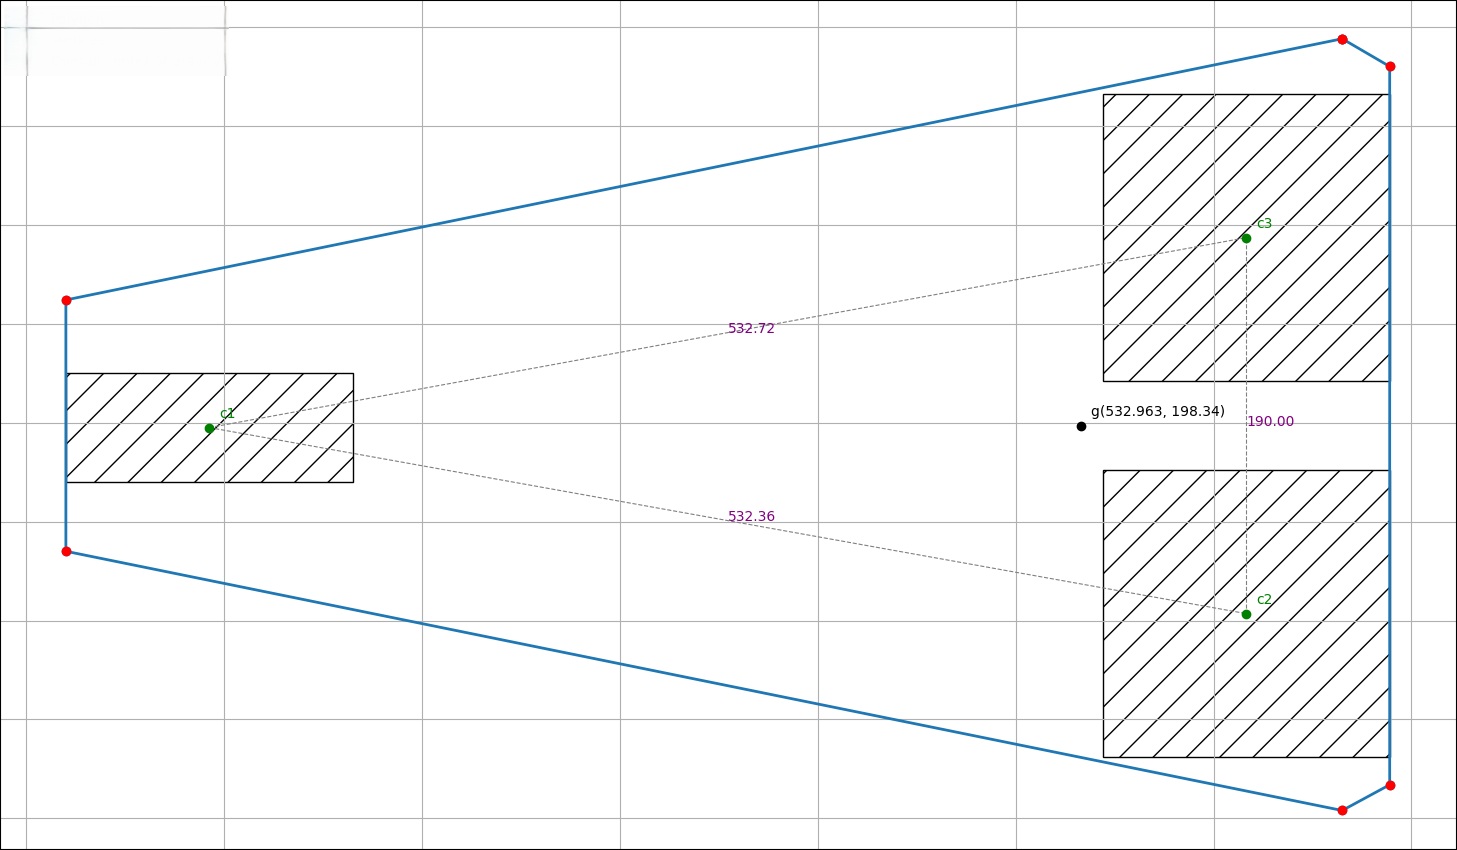
\includegraphics[width=1.8in]{figures/gurobi3.png} &
			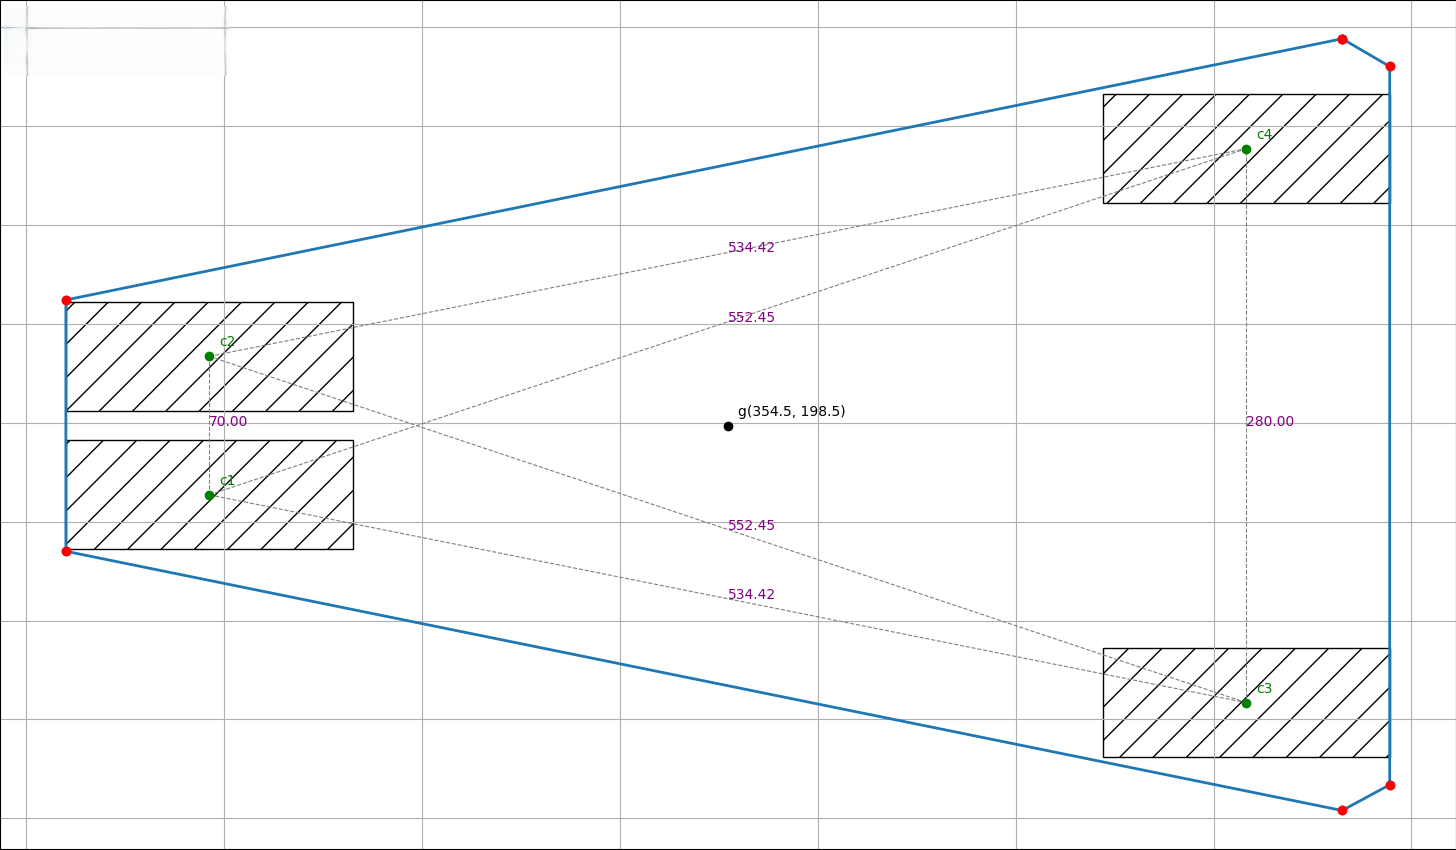
\includegraphics[width=1.8in]{figures/gurobi4.png} \\
			
			\bottomrule
		\end{tabular}
	\end{table}
	
	% =====================================================
	% TABLE 3: n = 5–10 (all solvers EXCEPT Gurobi f_iner)
	% =====================================================
	\begin{table}[p]
		\centering
		\small
		\caption{Visual results for solvers’ solutions using $\fdistsemi$ objective function ($\nmax = 5$--$10$).}
		\label{tab:visual_results_5_10_fdist}
		\renewcommand{\arraystretch}{1.5}
		
		\begin{tabular}{lcc}
			\toprule
			\multicolumn{1}{c}{} & \multicolumn{2}{c}{$\nmax$} \\
			\cmidrule(lr){2-3}
			\textbf{Solver} & 5 & 6--10 \\
			\midrule
			
			\raisebox{+6.0\height}{Chuffed} &
			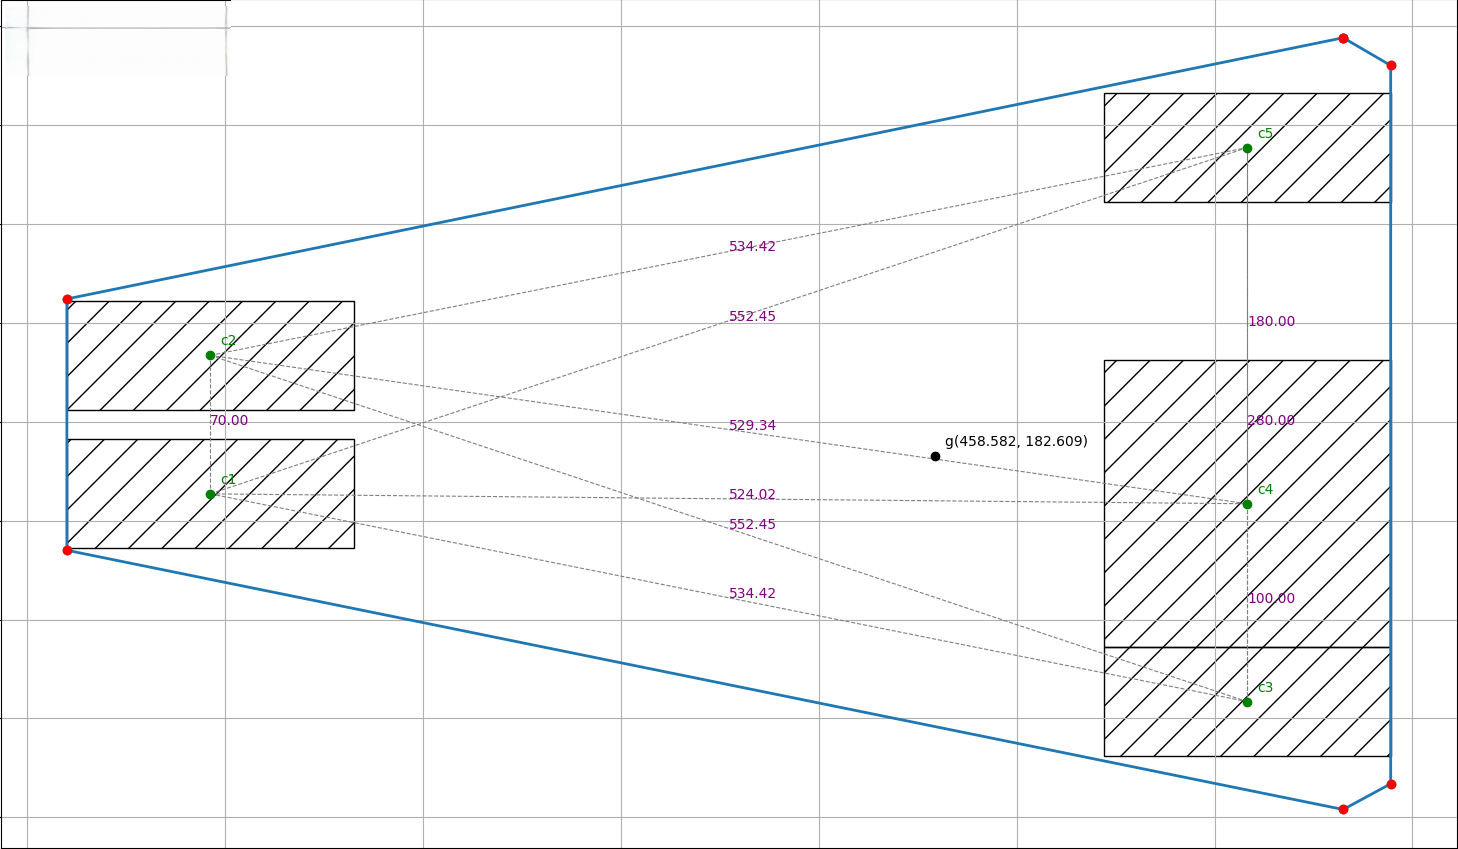
\includegraphics[width=1.8in]{figures/chuffed5.png} &
			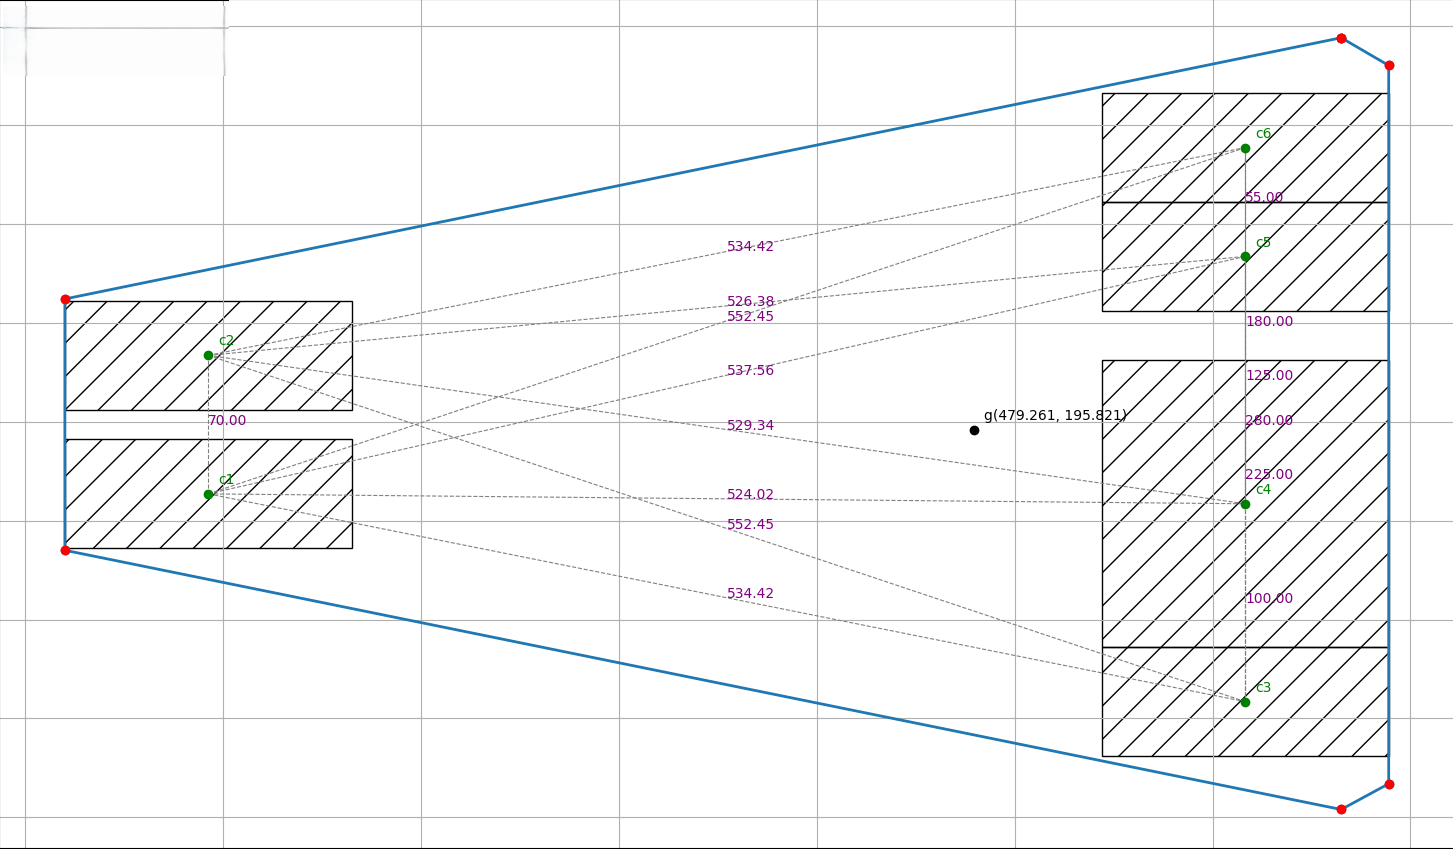
\includegraphics[width=1.8in]{figures/chuffed6.png} \\
			
			\raisebox{+6.0\height}{OR-Tools} &
			\raisebox{+12.0\height}{--} &
			\raisebox{+12.0\height}{--} \\
			
			\raisebox{+6.0\height}{Gurobi ($\fdistsemi$)} &
			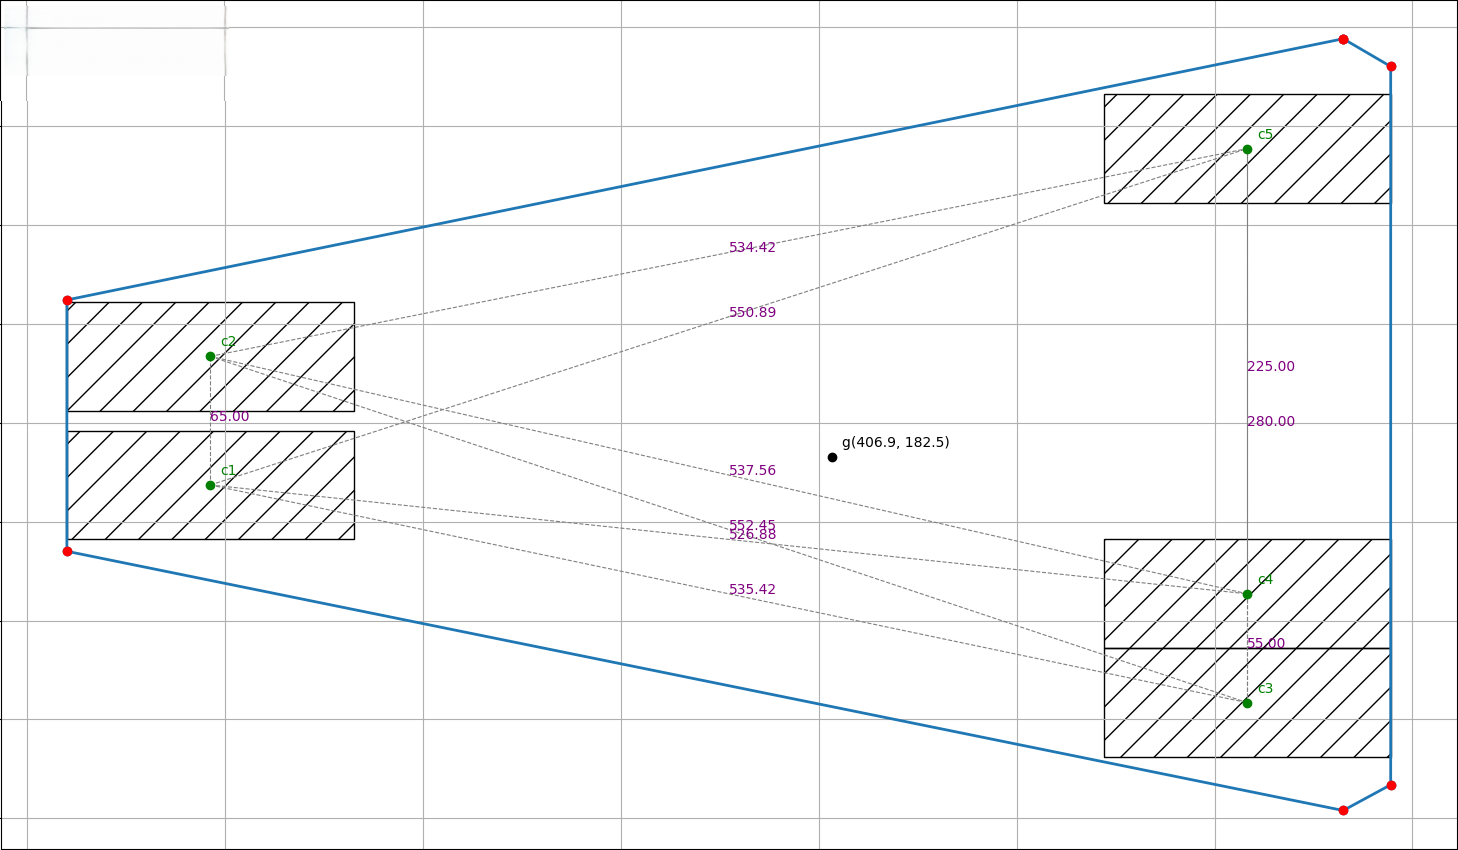
\includegraphics[width=1.8in]{figures/gurobi5.png} &
			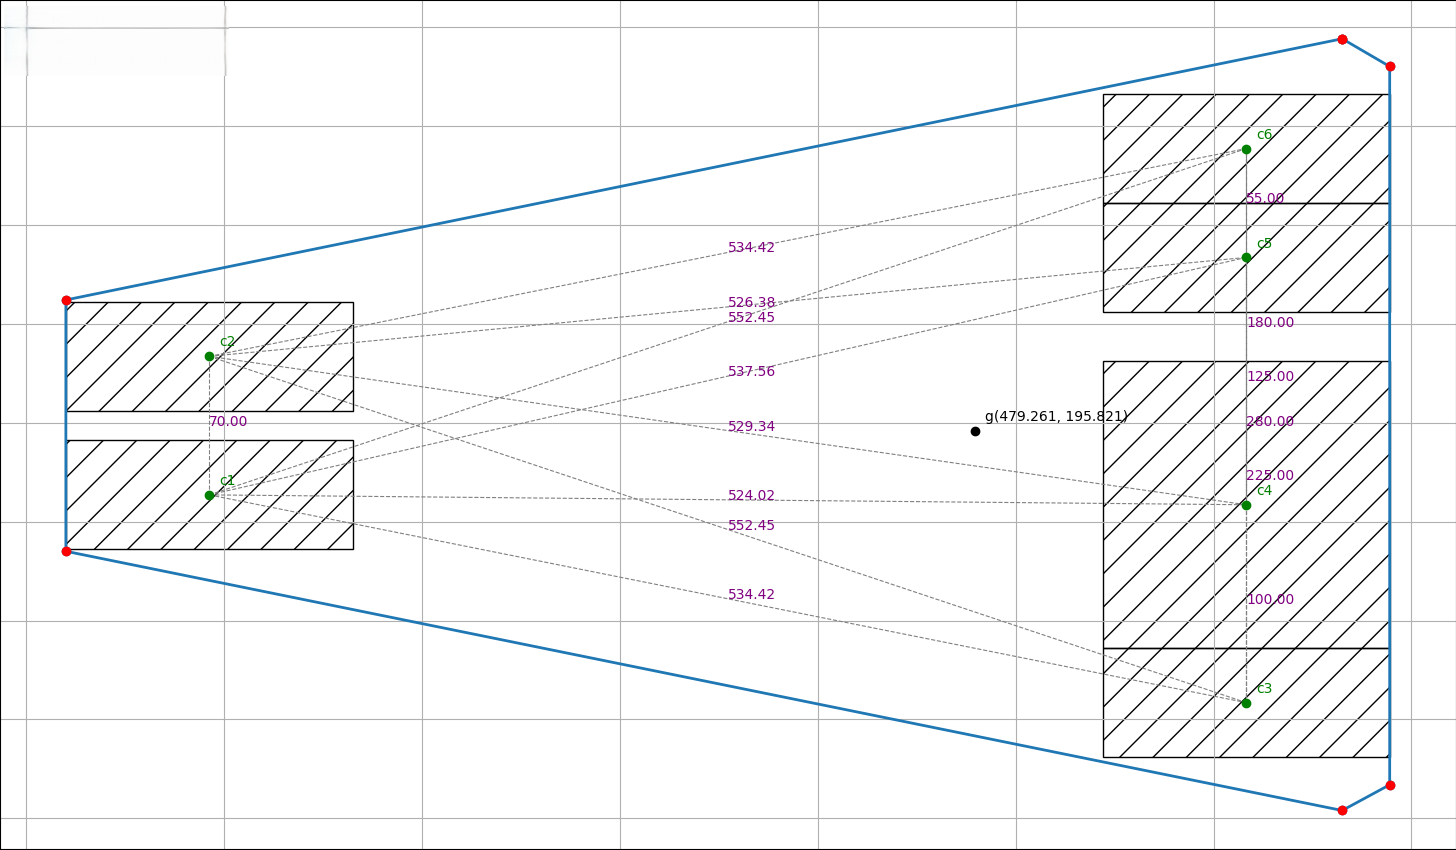
\includegraphics[width=1.8in]{figures/gurobi6.png} \\
			
			\bottomrule
		\end{tabular}
	\end{table}
	
		% =====================================================
	% TABLE 2: n = 2–4 (Gurobi f_iner ONLY)
	% =====================================================
	\begin{table}[p]
		\centering
		\small
		\caption{Visual results for Guorbi solver solutions using $\finer$ objective function ($\nmax = 2$--$4$).}
		\label{tab:visual_results_234_finer}
		\renewcommand{\arraystretch}{1.5}
		
		\begin{tabular}{lccc}
			\toprule
			\multicolumn{1}{c}{} & \multicolumn{3}{c}{$\nmax$} \\
			\cmidrule(lr){2-4}
			\textbf{Solver} & 2 & 3 & 4 \\
			\midrule
			
			Gurobi ($\finer$) &
			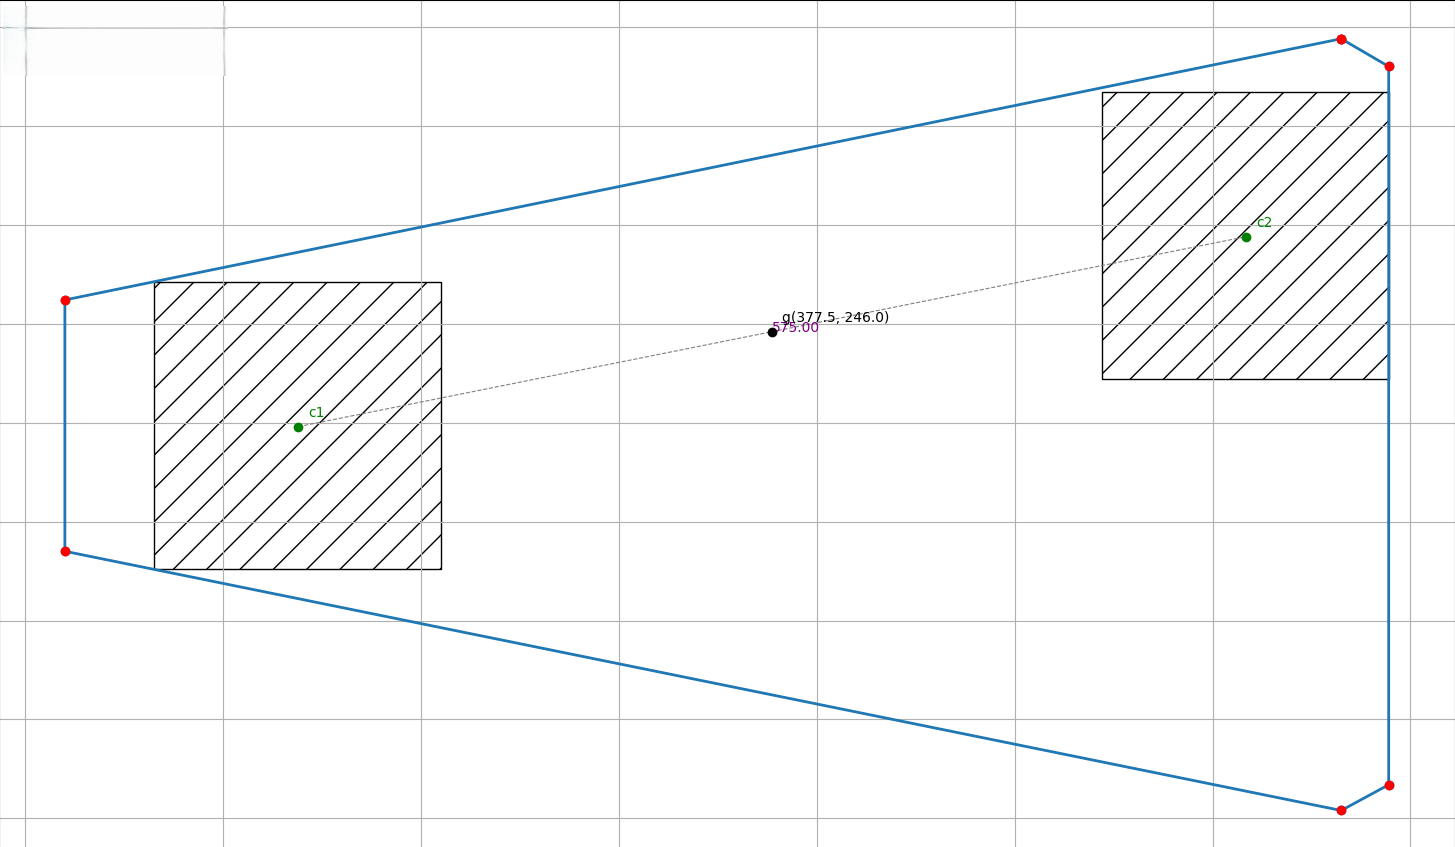
\includegraphics[width=1.8in]{figures/gurobi2_moments.png} &
			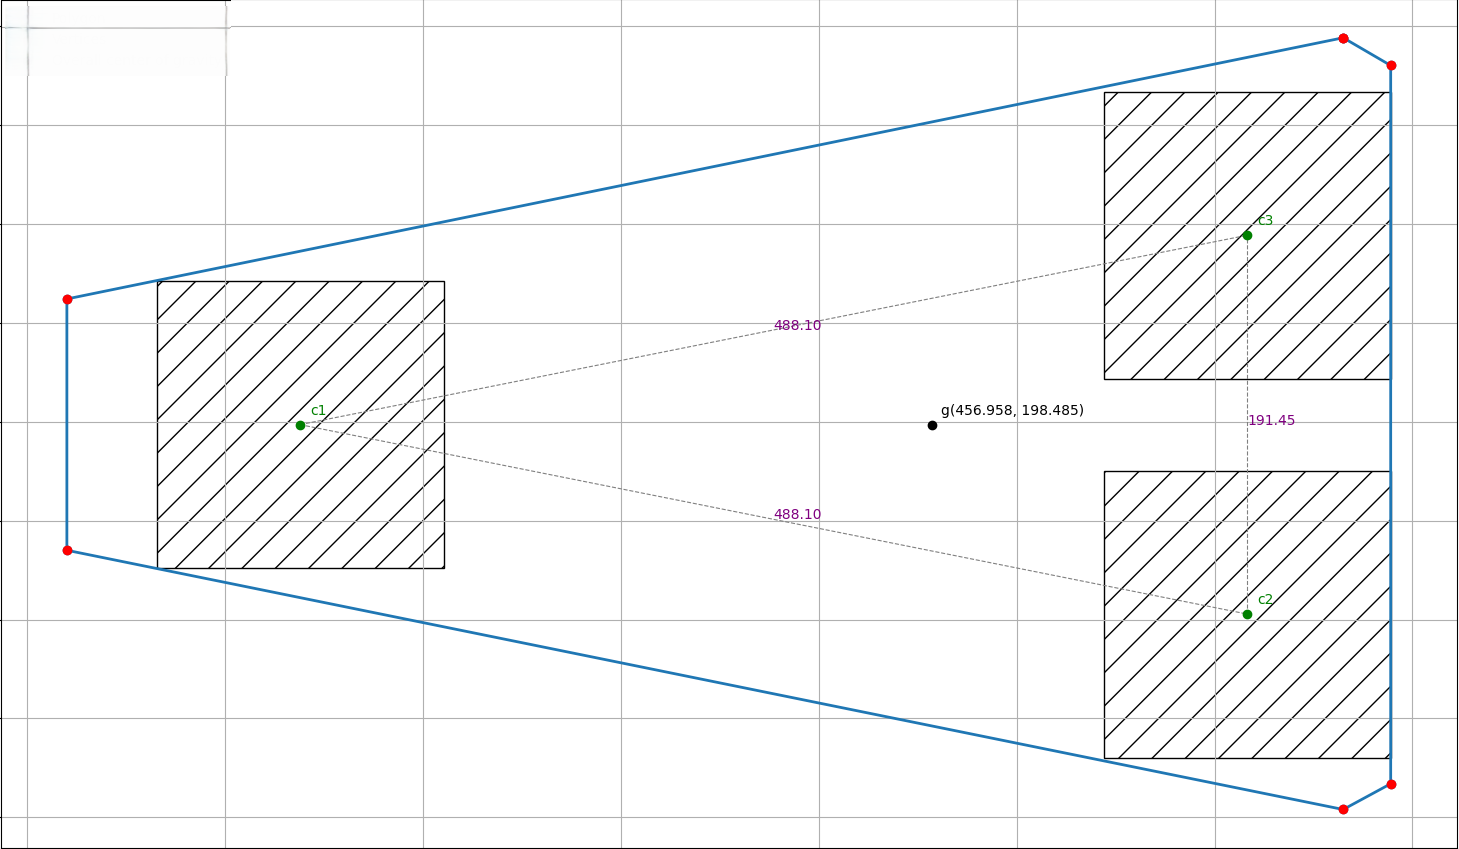
\includegraphics[width=1.8in]{figures/gurobi3_moments.png} &
			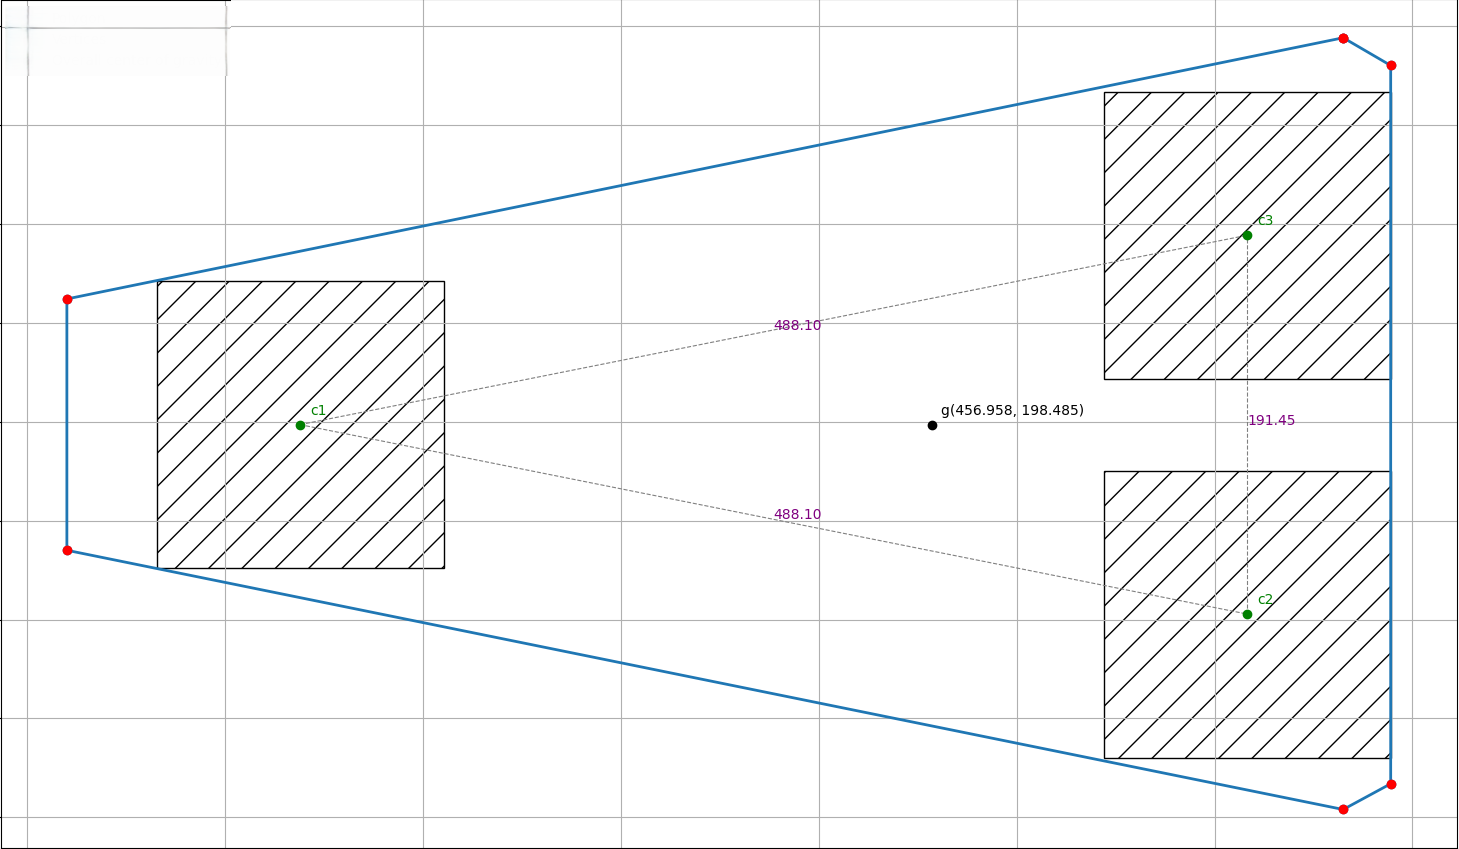
\includegraphics[width=1.8in]{figures/gurobi3_moments.png} \\
			
			\bottomrule
		\end{tabular}
	\end{table}
	
	% =====================================================
	% TABLE 4: n = 5–10 (Gurobi f_iner ONLY)
	% =====================================================
	\begin{table}[p]
		\centering
		\small
		\caption{Visual results for Guorbi solver solutions using $\finer$ objective function ($\nmax = 5$--$10$).}
		\label{tab:visual_results_5_10_finer}
		\renewcommand{\arraystretch}{1.5}
		
		\begin{tabular}{lcc}
			\toprule
			\multicolumn{1}{c}{} & \multicolumn{2}{c}{$\nmax$} \\
			\cmidrule(lr){2-3}
			\textbf{Solver} & 5 & 6--10 \\
			\midrule
			
			Gurobi ($\finer$) &
			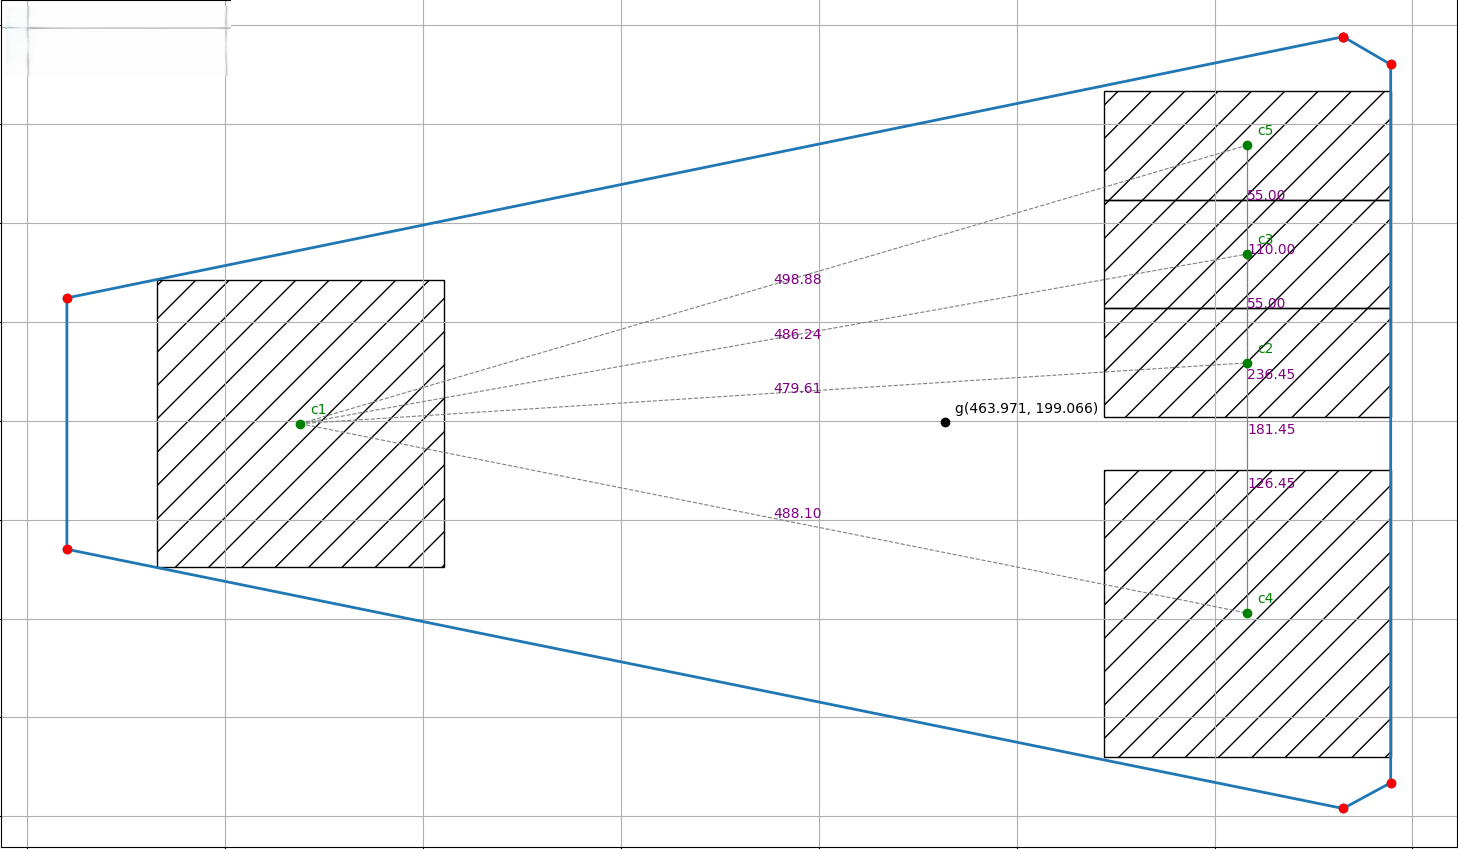
\includegraphics[width=1.8in]{figures/gurobi5_moments.png} &
			\raisebox{+12.0\height}{--} \\
			
			\bottomrule
		\end{tabular}
	\end{table}
	
	
	
\end{landscape}
	
	\chapter{Considering fixture rotations and extrusion areas}
	\label{chap:pt1_chapter6}

Having solved the simplified version of the problem, where fixture rotations  and areas to be extruded are not considered, using the CP model described in Chapter~\ref{chap:pt1_chapter5}, we now address the complete problem by incorporating both fixture rotations  and the presence of areas to be extruded within the workpiece.

The constraints remain the same as those described previously, with the additional requirement that fixtures must not be positioned beneath areas to be extruded. Therefore, the resulting constraints that need to be satisfied are:
\begin{enumerate}
	\item the number of placed fixtures must not exceed their availability;
	\item fixtures must satisfy the minimum safety distances;
	\item fixtures must lie within the boundaries of the workpiece and beneath its surface;
	\item fixtures must not overlap;
	\item fixtures must not be located beneath areas to be extruded.
\end{enumerate}

To clarify layout feasibility, Figure~\ref{fig:constraints_axample} illustrates examples of valid and invalid fixture placements. In the figure, fixture $F_6$ is invalid because it violates the minimum horizontal safety distance with respect to fixtures $F_3$ and $F_4$. Fixture $F_5$, on the other hand, is invalid because it is positioned beneath an area to be extruded.

\begin{figure}[t]
	\centering
	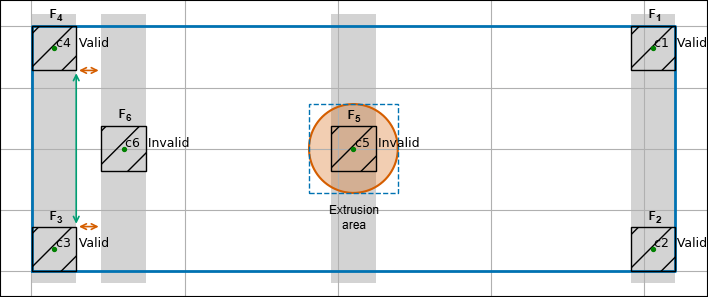
\includegraphics[width=0.65\linewidth]{figures/valid_invalid_positions_example.png}
	\caption{Example of valid and invalid fixture placements. For a fixture placement to be valid, the fixture must lie within the workpiece boundaries, satisfy the required safety distances from the other fixtures, and not be positioned beneath an area to be extruded.}
	\label{fig:constraints_axample}
\end{figure}

To address the complete problem, we extend the CP model introduced in Section~\ref{sec:first_cp_model} to handle the new constraint. We also formulate a new Mixed Integer Programming (MIP) model and propose a Q-learning based algorithm, comparing the three approaches on real-world test cases.

Both the CP and MIP models can be solved using appropriate solvers to obtain feasible layout. However, similarly to the Q-learning algorithm, neither approach accounts for fixture rotations, since allowing rotation angles other than multiples of $90^\circ$ significantly increases the number of possible configurations and makes the problem substantially harder to solve.

Moreover, inclined fixtures complicate overlap checking and, in CP solvers, require geometric approximations due to the lack of native support for continuous variables. For these reasons, fixture rotations are handled in a final refinement stage based on a Particle Swarm Optimization (PSO) meta-heuristic, which iteratively improves the initial solution, provided by the different approaches.

\section{Parameters and objective function}
\label{sec:second_parameters}
The problem parameters extend those introduced in Section~\ref{sec:first_parameters} with information related to the areas to be extruded. 

All the proposed solution strategies are defined over the same set of input parameters, listed below:

\begin{itemize}
	\item the width $\wtab$ and height $\htab$ of the machine worktable;
	\item the minimum horizontal distance $\wmin$ between two fixtures placed on different bars;
	\item the minimum vertical distance $\hmin$ between two fixtures placed on the same bar;
	\item the number $\ntypes$ of different fixture types;
	\item the number $\nfix_i$ of available fixtures for each type $i \in [1..\ntypes]$;
	\item the total number of available fixtures $\nfix = \sum_{i=1}^{\ntypes} \nfix_i$;
	\item the minimum $\nmin$ and maximum $\nmax$ number of fixtures to place;
	\item the width $\wfix_i$ and height $\hfix_i$ of each fixture of type $i$;
	\item the workpiece shape, by a set of linear inequalities of the form $\mathtt{a}\,x + \mathtt{b}\,y + \mathtt{c} \leq 0$;
	\item the number $\numext$ of areas to be extruded;
	\item the width $\ewside_i$, height $\ehside_i$, and the coordinates $(\xext_i, \yext_i)$ of the lower-left corner of the smallest axis-aligned rectangle enclosing each area $i \in [1..\numext]$ to be extruded.
\end{itemize}

To facilitate the solving process, areas to be extruded are approximated by their minimum bounding rectangles. In practice, these areas typically correspond to simple geometries, such as circles, rectangles, or ellipses, while more complex shapes are usually refined manually.

Compared with the simplified formulation, we also introduce in the parameters the minimum vertical distance between fixtures. This parameter was previously omitted to allow the placement of multiple fixtures beneath the workpiece and to facilitate the comparison between $\fdistsemi$ and $\finer$ for increasing values of $\nmax$ (see Section~\ref{sec:case_study}).

To evaluate the quality of a fixture layout, two objective functions are considered $\fdistarea$ and $\finer$. 

The CP and MIP models optimize the objective function $\fdistarea$, which maximizes the sum of the pairwise Manhattan distances between fixture centroids, augmented by the total area of the selected fixtures:

\begin{equation}
	\fdistarea = \sum_{1 \le i < j \le n} \left(|cx_i - cx_j| + |cy_i - cy_j|\right) + \sum_{k=1}^{n} (\wfix_{t_k} \cdot \hfix_{t_k})
	\label{eq:f_dist_area}
\end{equation}

We adopt the area term instead of the semi-perimeter to prioritize fixtures with larger contact surfaces. We empirically verified that this approach provides a stronger surrogate for the inertia objective in more complex geometries. In the experiments of Section~\ref{sec:evaluation}, the Pearson correlation  coefficient~\cite{benesty2009pearson} between $\fdistarea$ and $\finer$ when using the area-based formulation is higher (0.79) than the semi-perimeter-based one (0.39).

Unlike the CP and MIP models, the Q-learning algorithm is not affected by the nonlinear operations required to evaluate $\finer$. Consequently, it does not rely on the alternative objective function; instead, it directly incorporates the moments of inertia into the reward returned by the environment.

\section{CP model}
\label{sec:cp_model}

We formulate the model by extending the CP formulation presented in Section~\ref{sec:first_cp_model} through a revised definition of the decision variables and a reformulation of some constraints, which will be presented in the following sections. 

\subsection{Variables}
\label{sec:second_cp_variables}

The fixture placement and type are represented by three arrays of integer decision variables, $x$, $y$, and $t$, for $i = 1,\ldots,\nmax$:
\begin{itemize}
	\item $ (x_i,y_i) \in [0..\wtab]\times [0..\htab] $ denotes the coordinates of the lower-left corner of the $i$-th fixture;
	\item $ t_i \in [0..\ntypes] $ denotes the type of the $i$-th fixture, where type $0$ represents an unused fixture.
\end{itemize}

For each fixture type $i \in [1..\ntypes]$, an integer variable $n_i \in [0..\nfix_i]$ denotes the number of selected fixtures of type $i$, and a variable $n \in [\nmin..\nmax]$ represents the total number of selected fixtures.

Compared with the formulation presented in~\ref{sec:first_cp_model}, the arrays $x$ and $y$ and the variable $n$ are now bounded by $\nmax$, rather than by $\nfix$, since the maximum number of fixtures that can be placed is known for each workpiece and $\nmax \leq \nfix$ this tighter bound reduces the search space.


\subsection{Constraints}
\label{sec:second_cp_cons}

For each fixture type $i \in [1..\ntypes]$, the \texttt{count} global constraint is used to compute the number of occurrences of value $i$ in the array $t$:

\[
n_i = \texttt{count}(t,i)
\]

The total number of selected fixtures is then defined as

\[
n = \sum_{i=1}^{\ntypes} n_i
\]

Fixture availability is enforced by requiring that the number of selected fixtures of each type does not exceed the number available:

\[
n_i \leq \nfix_i, \qquad \forall i \in [1..\ntypes]
\]

Since not all available fixtures must necessarily be used, we enforce the following invariant:
\[
(i > n) \iff (x_i = \wtab \;\wedge\; y_i = \htab \;\wedge\; t_i = 0), \qquad \forall i \in [1..\nmax]
\]

This invariant ensures that all unused fixtures are assigned the dummy type $0$ and placed at the dummy location $(\wtab,\htab)$, which lies outside the feasible region.

We guarantee that exactly $\nmax-n$ fixtures remain unused by imposing

\[
\texttt{count}(t,0) = \nmax - n
\]


The workpiece shape is defined by linear inequalities of the form $ \mathtt{a}\,x + \mathtt{b}\,y + \mathtt{c} \leq 0 $.
To ensure that each selected fixture $ i $ is placed within the workpiece, we must satisfy
$
\mathtt{a}\,x'_i + \mathtt{b}\,y'_i + \mathtt{c} \leq 0,
$
where $x'_i$ and $y'_i$ are defined as in Section~\ref{sec:first_constraints}.

Areas to be extruded are approximated by axis-aligned rectangles. The non-overlap between these areas and the fixtures is enforced using the \texttt{diffn} global constraint~\cite{DBLP:journals/constraints/BeldiceanuCDP07}:

\[
\texttt{diffn}\big(
x \oplus \xext,\;
y \oplus \yext,\;
[\wfix_{t_i} \mid i \in [1..n]] \oplus \ewside,\;
[\hfix_{t_i} \mid i \in [1..n]] \oplus \ehside
\big)
\]

\noindent where $ \oplus $ denotes array concatenation. Specifically, we use the \emph{non-strict} version of \texttt{diffn}, ignoring the unused fixtures.

To enforce the minimum \emph{vertical} distance $ \hmin $ between fixtures placed on the same bar, and the minimum \emph{horizontal} distance $ \wmin $ between fixtures placed on different bars we impose:

\begin{equation*}
	\begin{aligned}
		&\forall\,1 \le i < j \le n:\quad
		\begin{cases}
			y_i + \hfix_{t_i} + \hmin \le y_j
			\\[-0.2ex]
			\quad\vee\quad
			y_j + \hfix_{t_j} + \hmin \le y_i,
			& \text{if } cx_i = cx_j
			\\[1ex]
			x_i + \wfix_{t_i} + \wmin \le x_j,
			& \text{if } cx_i \ne cx_j
		\end{cases}
	\end{aligned}
\end{equation*}

\noindent where $cx_i$ denotes the $x$-coordinate of the centroid of fixture $ i $. Centroid coordinates are used instead of lower-left coordinates because fixtures may be wider than their supporting bar: while $ x_i $ may fall outside the horizontal span of the bar, the centroid $ cx_i $ always lies within it.

To compute the fixture centroid coordinates while preserving integer-valued variables, the coordinates are obtained using integer division of the fixture dimensions. For each fixture $i \in [1..\nmax]$, we define:

\begin{align*}
	cx_i = x_i + \left\lfloor \frac{\wfix_{t_i}}{2} \right\rfloor \quad
	cy_i = y_i + \left\lfloor \frac{\hfix_{t_i}}{2} \right\rfloor 
\end{align*}

To improve the propagation of the integer division, the following redundant linear constraints were introduced:

\begin{align*}
	2 \cdot cx_i - 2 \cdot x_i = \wfix_{t_i} - (\wfix_{t_i} \bmod 2) \\
	2 \cdot cy_i - 2 \cdot y_i = \hfix_{t_i} - (\hfix_{t_i} \bmod 2)
\end{align*}

Finally, the model exhibits symmetries whenever fixtures of the same type are permuted without changing their spatial arrangement. To eliminate these equivalent solutions, a lexicographic ordering is imposed on the fixture positions using the \texttt{lex\_chain} global constraint:

\[
(x_{i-1},y_{i-1}) \preceq (x_i,y_i)
\qquad i \in [2..\nmax]
\]

\section{MIP model}
\label{sec:mip_model}

In this section, we present the Mixed-Integer Programming (MIP) formulation for the fixture layout optimization problem. Compared to the CP model described in Section~\ref{sec:cp_model}, all the constraints are expressed in linear form, and the positional decision variables are continuous rather than discrete.

This important relaxation comes from the nature of MIP solving which, unlike most CP solvers, naturally handles non-negative continuous variables.
Nevertheless, a number of discrete variables are still required to capture the combinatorial structure of the problem, as detailed below.

\subsection{Variables}
Variables $x_i$ and $y_i$ for $i=1,\dots,\nmax$ have exactly the same semantics as those defined in Section~\ref{sec:second_cp_variables}, with the only difference that they are now continuous reather than discrete.

Fixture types are encoded with a 0-1 matrix $T$ of size $\nmax \times \ntypes$, whose semantics is:
\[
T_{i,j} =
\begin{cases}
	1 & \text{if fixture $i$ is selected and has type $j$,} \\
	0 & \text{otherwise.}
\end{cases}
\]

The linearization of the constraints comes at the expense of the introduction of auxiliary 0-1 variables, detailed as follows:
\begin{itemize}
	\item $\used_i$, denoting whether fixture $i$ is selected;
	\item $\samebar_{i,j}$, denoting whether fixtures $i$ and $j$ lie on the same bar;
	\item $\aboveinbar_{i,j}$, $\belowinbar_{i,j}$, denoting whether fixture $i$ is above or below fixture $j$ on the same bar;
	\item $\nooverlapabove_{i,j}, \nooverlapbelow_{i,j}, \nooverlapleft_{i,j}, \nooverlapright_{i,j}$, indicating whether fixture $i$ is positioned above, below, to the left, or to the right of fixture $j$, respectively.
	\item $\aboveext_{i,j}$, $\belowext_{i,j}$, $\leftext_{i,j}$, $\rightext_{i,j}$ indicating whether fixture $i$ is positioned above, below, to the left, or to the right of an area $j$ to be extruded, respectively.
\end{itemize}

We also define auxiliary variables $w_i$, $h_i$ and $t_i$ to denote, respectively, the width $w_i$, the height $h_i$, and the type $t_i$ of each fixture.

\subsection{Constraints}
For each fixture $i \in [1..\nmax]$ we impose:
\[
\used_i = \sum_{j=1}^{\ntypes} T_{i,j} \qquad
w_i = \sum_{j=1}^{\ntypes} \wfix_j\cdot T_{i,j} \qquad
\]
\[
h_i = \sum_{j=1}^{\ntypes} \hfix_j\cdot T_{i,j} \qquad
t_i = \sum_{j=1}^{\ntypes} j \cdot T_{i,j}
\]

These equations ensure that the width, height, and type assigned to each fixture are consistent and that unused fixtures have dimensions and type equal to $0$.

To enforce availability constraints, we impose:
\[
\sum_{i=1}^{\nmax} T_{i,j} \le \nfix_j, \quad \forall j \in [1..\ntypes] \qquad\qquad
\nmin \le \sum_{i=1}^{\nmax} \used_i \le \nmax
\]

To determine whether two fixtures lie on the same bar for all $i \in [1..\nmax]$ and $j \in [i+1..\nmax]$ we define the following constraints:
\[
\begin{aligned}
	&\samebar_{i,j} \le \used_i \qquad \samebar_{i,j} \le \used_j \\
	&\samebar_{i,j} = \aboveinbar_{i,j} + \belowinbar_{i,j}\\
	&cx_i - cx_j \le M (1 - \samebar_{i,j}) \qquad cx_j - cx_i \le M (1 - \samebar_{i,j}) \\
\end{aligned}
\]

\noindent where $M = \wtab \cdot \htab$ is the \emph{``big-M''} constant. To enforce the appropriate safety distances:

\[
\begin{aligned}
	&cx_i + \wmin \le cx_j + M(\samebar_{i,j} + \nooverlapright_{i,j}) \\
	&cx_j + \wmin \le cx_i + M(\samebar_{i,j} + \nooverlapleft_{i,j}) \\
	&y_i + h_i + \hmin - y_j \le M (1 - \aboveinbar_{i,j}) \\
	&y_j + h_j + \hmin - y_i \le M (1 - \belowinbar_{i,j})
\end{aligned}
\]

To prevent overlap between fixtures, for all $i,j \in [1..\nmax]$ with $i < j$, we impose:
\[
\begin{aligned}
	&\nooverlapabove_{i,j} + \nooverlapbelow_{i,j} +
	\nooverlapleft_{i,j} + \nooverlapright_{i,j} \ge 1 \\
	&x_i + w_i \le x_j + M (1 - \nooverlapleft_{i,j}) \qquad
	&y_i + h_i \le y_j + M (1 - \nooverlapbelow_{i,j}) \\
	&x_j + w_j \le x_i + M (1 - \nooverlapright_{i,j}) \qquad
	&y_j + h_j \le y_i + M (1 - \nooverlapabove_{i,j})
\end{aligned}
\]

The same constraints are applied to prevent overlap between fixtures and areas to be extruded. For each fixture $i \in [1..\nmax]$ and extrusion area $j \in [1..\numext]$, the above inequalities are instantiated using the variables $\aboveext_{i,j}$, $\belowext_{i,j}$, $\leftext_{i,j}$, and $\rightext_{i,j}$.

The workpiece is defined by linear inequalities of the form $\mathtt{a}x_i + \mathtt{b}y_i + \mathtt{c} \leq 0$, so for each fixture $i \in [1..\nmax]$ we impose
$\mathtt{a}x'_i + \mathtt{b}y'_i + \mathtt{c} \leq 0$ where $x'_i$ and $y'_i$ are defined as in Section~\ref{sec:first_constraints}.

To break symmetries, we impose an ordering on fixture types: $t_i \ge t_{i+1}$ for $i \in [1..\nmax-1]$.

\noindent We linearize $\fdistarea$ with a big-M formulation unfolding each term of the form $u=|v|$ into: $$u \ge v ~\wedge~ u \ge -v ~\wedge~ u \leq v + M (1 - b)  ~\wedge~ u \leq -v + M b~\wedge~ b\in\{0,1\}.$$

\section{Q-learning algorithm}

The solutions obtained using the CP and MIP models are compared with those produced by a Q-learning based algorithm. This comparison provides insight into the differences between the layouts generated by exact optimization methods and those obtained through a learning-based strategy.

In Q-learning an agent estimates the action-value function $Q(s,a)$, which represents the expected \emph{cumulative discounted reward} associated with taking action $a$ in state $s$ and subsequently following the optimal policy $\pi$~\cite{watkins1992q}.

In our formulation, the environment corresponds to the considered workpiece. At each decision step, the state of the environment is defined as:

\[
s_t=(n_t,fix_t),
\]

\noindent where $n_t$ is the number of fixtures already placed at step $t$, while
$fix_t=[fix_t^{1},\,fix_t^{2},\\ \,\ldots,\,fix_t^{\ntypes}]$
is an integer array of size $\ntypes$, whose components denote the remaining availability of the different fixture types.

An action consists of selecting a fixture type together with a feasible centroid position:

\[
a_t=(type_t,(cx_t,cy_t)).
\]

The fixture centroid is used as the reference point for positioning instead of the lower-left corner adopted in the CP and MIP models, since it simplifies both the enforcement of the horizontal and vertical safety-distance constraints, as described in Section~\ref{sec:second_cp_cons}, and the identification of feasible actions.

The action to be executed is selected according to an \textit{$\epsilon$-greedy policy}~\cite{sutton1998reinforcement}. At each decision step, the agent selects the action with the highest estimated $Q$-value with probability $1-\epsilon$, whereas with probability $\epsilon$ it selects a random action, balancing exploration and exploitation of the environment.

The Q-learning based procedure adopted for fixture layout optimization is described in Algorithm~\ref{alg:qlearning_fixtures}. The algorithm takes as inputs the number of training episodes $E$, the maximum number of steps per episode $T$, the learning rate $\alpha$, the discount factor $\gamma$, the exploration rate $\epsilon$, and the exploration decay factor $\rho$. The output is the best feasible fixture layout $\mathcal{L}^{*}$ obtained by applying the learned policy $\pi$.

\begin{algorithm}[ht]
	\footnotesize
	\caption{Q-learning for Fixture Layout Optimization}
	\label{alg:qlearning_fixtures}
	\begin{algorithmic}[1]
		
		\Require Number of episodes $E$, maximum number of steps per episode $T$, learning rate $\alpha$, discount factor $\gamma$, exploration rate $\epsilon$, exploration decay factor $\rho$
		\Ensure Best feasible layout $\mathcal{L}^*$
		
		\State Compute all candidate centroid positions
		\label{alg:q_init_start}
		\State Remove centroid positions violating the constraints and set $\mathcal{A}(s_1)$
		\State Initialize $Q(s,a)=0$
		\State $\mathcal{L}^* \gets \emptyset$
		\label{alg:q_init_end}
		
		\For{$ep=1$ to $E$}
		\label{alg:q_iteration_start}
		
		\For{$t=1$ to $T$}
		
		% \State Compute the feasible action set $\mathcal{A}(s_t)$
		
		\If{$\mathcal{A}(s_t)=\emptyset$}
		\State \textbf{break}
		\EndIf
		\label{alg:q_iteration_end}
		
		\If{random number $<\epsilon$} \Comment{exploration}
		\label{alg:q_policy_start}
		\State Select a random feasible action
		$a_t \in \mathcal{A}(s_t)$
		\Else \Comment{exploitation}
		\State Select
		$a_t=\arg\max\limits_{a\in\mathcal{A}(s_t)}Q(s_t,a)$
		\EndIf
		
		\State Perform action $a_t$ by placing the selected fixture
		\label{alg:q_policy_end}
		
		\State Recompute the feasible action set $\mathcal{A}(s_{t+1})$ 
		\label{alg:q_reset_action}
		
		\State Compute reward $r_t$ according to Eq.~\ref{eq:reward}
		\label{alg:q_update_start}
		
		\State Observe successor state $s_{t+1}$
		
		\State $Q(s_t,a_t) \gets Q(s_t,a_t) + \alpha \left[r_{t+1} + \gamma \max_{a_{t+1}}Q(s_{t+1},a_{t+1}) - Q(s_t,a_t) \right]$
		
		\State $s_t \gets s_{t+1}$
		\State Update $\pi$ with $a_t$
		\label{alg:q_update_end}
		
		\EndFor
		
%		\If{$\mathcal{L}_{ep}$ is better than $\mathcal{L}^*$}
%		\label{alg:q_new_ep_start}
%		\State $\mathcal{L}^* \gets \mathcal{L}_{ep}$
%		\EndIf
		\State $\epsilon \gets \rho\,\epsilon$
		\label{alg:q_new_ep_start}
		\State Reset the environment to the initial state $s_1$
		\State Reset the action space to $\mathcal{A}(s_1)$
		\label{alg:q_new_ep_end}
		
		\EndFor
		
		\State Evaluate the learned policy $\pi$
		\label{alg:q_evaluate_start}
		\State \textbf{return} $\mathcal{L}^*$
		\label{alg:q_evaluate_end}
		
	\end{algorithmic}
\end{algorithm}

Given the fixture dimensions, it is known \emph{a priori} that some positions within the workpiece cannot accommodate a fixture, particularly those near the workpiece boundary or close to areas to be extruded. During the initialization phase, in lines~\ref{alg:q_init_start}--\ref{alg:q_init_end} of Algorithm~\ref{alg:qlearning_fixtures}, centroid positions that would result in fixtures extending outside the workpiece boundaries or overlapping areas to be extruded are removed from the set of possible actions $\mathcal{A}(s_t)$, considering the dimensions of the smallest fixture as reference.

\begin{figure}[t]
	\centering
	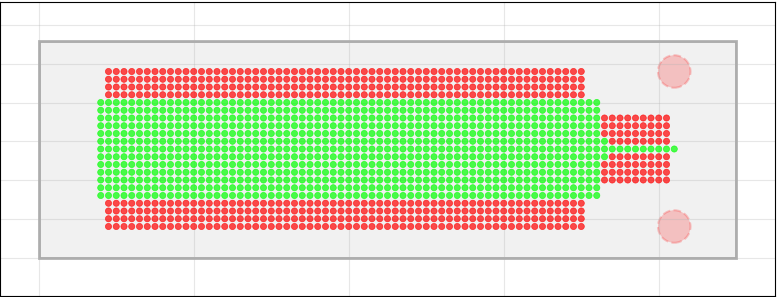
\includegraphics[width=0.5\linewidth]{figures/q_learning_actions.png}
	\caption{Example of the available actions for a given workpiece. Green dots represent centroid positions where both square and rectangular fixtures can be placed, whereas red dots represent positions where only rectangular fixtures can be placed. The workpiece area is highlighted in light gray, while the areas to be extruded are highlighted in red.}
	\label{fig:q_learning_actions}
\end{figure}

Figure~\ref{fig:q_learning_actions} shows an example of the set of feasible actions for a given workpiece, considering two available fixture types: square and rectangular. Green dots indicate centroid positions where both fixture types can be placed, whereas red dots indicate positions where only rectangular fixtures can be placed.

The algorithm iterates over the training episodes and the corresponding steps. An episode terminates when no feasible actions remain or the maximum number of steps is reached, as reported in lines~\ref{alg:q_iteration_start}--\ref{alg:q_iteration_end} of Algorithm~\ref{alg:qlearning_fixtures}.

The agent selects actions according to the $\epsilon$-greedy policy (lines~\ref{alg:q_policy_start}--\ref{alg:q_policy_end} of Algorithm~\ref{alg:qlearning_fixtures}), balancing the exploration of new placements with the exploitation of previously learned actions.

Each action selected is evaluated through the reward associated with the transition from $s_t$ to $s_{t+1}$. The reward function combines the improvement obtained in the moment of inertia with additional terms promoting layouts composed of a larger number of fixtures, larger fixture dimensions, and increased spatial separation between fixtures:

\begin{equation}
	r_{t+1}
	=
	\lambda_{\mathrm{iner}}\,\Delta\finer
	+
	\lambda_n n_{t+1}^{2}
	+
	\lambda_d\bar d
	+
	\begin{cases}
		b_{\nmin}, & \text{if } n_{t+1}\geq\nmin,\\
		0, & \text{otherwise}.
	\end{cases}
	\label{eq:reward}
\end{equation}

\noindent in the equation: 
\begin{itemize} 
	\item $\Delta\finer$ is the variation of $\finer$ between the previous and current states;
	\item $n_{t+1}$ is the number of fixtures in the resulting layout. The quadratic term promotes layouts with a larger number of fixtures;
	\item $\bar d$ is the average Euclidean distance between the newly placed fixture and the previously placed fixtures,  promoting layouts with a larger spatial separation;
	\item $\lambda_{\finer}$, $\lambda_n$, and $\lambda_d$ are weighting coefficients balancing the contribution of the different reward components;
	\item $b_{\nmin}$ is an additional feasibility bonus assigned when the minimum required number of fixtures, $\nmin$, has been placed.
\end{itemize}

After each fixture placement, all candidate centroid positions that no longer satisfy the safety-distance constraints are removed from the feasible action set, as reported in line~\ref{alg:q_reset_action} of Algorithm~\ref{alg:qlearning_fixtures}. Consequently, the action set progressively shrinks as the layout is constructed, ensuring that all geometric constraints are satisfied.

The only constraint that cannot be enforced by restricting the feasible action set is the placement of the minimum number of required fixtures $\nmin$. For this reason, the feasibility bonus $b_{\nmin}$ is included in the reward function to encourage the agent to generate layouts satisfying this constraint.

After executing the selected action, and obtained the corresponding reward, the $Q$-function value associated with state $s_t$ and action $a_t$ is evaluated and the learned policy $\pi$ is updated (lines~\ref{alg:q_update_start}--\ref{alg:q_update_end} of Algorithm~\ref{alg:qlearning_fixtures}).

Once an episode has ended, the environment is arranged for the next episode, as reported in lines~\ref{alg:q_new_ep_start}--\ref{alg:q_new_ep_end} of Algorithm~\ref{alg:qlearning_fixtures}.

Finally, after all training episodes have been completed, the learned policy is evaluated to obtain the fixture layout for the considered workpiece, as illustrated in lines~\ref{alg:q_evaluate_start}--\ref{alg:q_evaluate_end} of Algorithm~\ref{alg:qlearning_fixtures}.


\section{Particle Swarm Optimization algorithm}
\label{sec:pso_algorithm}
Particle Swarm Optimization (PSO) is employed to explicitly account for fixture rotation, considering as objective function $\finer = J_\xi + J_\eta$.

PSO is particularly well suited to this refinement phase due to its fast convergence and strong global search capability in high-dimensional and multi-objective optimization problems. Additionally, its simple structure, limited number of control parameters, and ease of hybridization enable robust optimization across diverse manufacturing, scheduling, and design applications when compared with Genetic Algorithms (GA), Simulated Annealing (SA), and gradient-based methods~\cite{kulkarni2015particle}.

In our case, the position of each particle $s \in [1..\swarmsize]$ is represented by a matrix $P_s$ with four rows and $\nmax$ columns. Each column of $P_s$ corresponds to a fixture, while each row encodes one of the problem decision variables:
\begin{itemize}
	\item $P_s[1,j]$: the $x$-coordinate of the lower-left corner of the $j$-th fixture;
	\item $P_s[2,j]$: the $y$-coordinate of the lower-left corner of the $j$-th fixture;
	\item $P_s[3,j]$: the type $t$ associated with the $j$-th fixture;
	\item $P_s[4,j]$: the rotation angle $\alpha$ of the $j$-th fixture.
\end{itemize}

Each position matrix $P_s$ represents a candidate solution associated with particle $s$. The availability of an initial solution obtained from the CP model, the MIP model, or the Q-learning algorithm, ensures that the swarm is initialized from feasible layouts.


\begin{algorithm}[htbp]
	\footnotesize
	\caption{Particle Swarm Optimization for Fixture Layout Optimization}
	\label{alg:pso_fixtures}
	\begin{algorithmic}[1]
		\Require Swarm size $\swarmsize$, maximum number of iterations $\maxiter$, inertia weight $w$, cognitive coefficient $c_1$,
		social coefficient $c_2$, variable bounds, initial solution $P_0$, maximum number of fixtures $\nmax$
		\Ensure Feasible solution $P^*$ not worse than $P_0$
		
		\For{$s = 1$ to $\swarmsize$}
		\label{alg:start_init}
		\If{$s = 1$}
		\State $P^* \gets P^*_s \gets P_s \gets P_0$
		\Else
		\State $P^*_s \gets P_s \gets P_0 + \text{random perturbation}$
		\EndIf
		\label{alg:end_init}
		
		\If{$cv(P_s)=0$}
		\label{alg:start_init_eval}
		\If{$\finer(P_s)>\finer(P^*)$}
		\State $P^*\gets P_s$
		\EndIf
		\EndIf
		\label{alg:end_init_eval}
		
		\State Randomly initialize velocity matrix $V_s$
		\EndFor
		
		\For{$k=1$ to $\maxiter$}
		\For{$s=1$ to $\swarmsize$}
		\For{$i=1$ to $4$}
		\For{$j=1$ to $\nmax$}
		\Comment{Update velocity and position}
		\State Randomly generate $r_1,r_2\in[0,1]$
		\label{alg:start_pso_update}
		\State $V_s[i,j]\gets wV_s[i,j]+c_1r_1(P^*_s[i,j]-P_s[i,j])+c_2r_2(P^*[i,j]-P_s[i,j])$
		\State $P_s[i,j]\gets P_s[i,j]+V_s[i,j]$
		\label{alg:end_pso_update}
		\EndFor
		\EndFor
		
		\For{$j=1$ to $\nmax$}
		\If{fixture $j$ lies outside the workpiece}
		\label{alg:start_fixing_geom}
		\State Identify the nearest workpiece vertex and the fixture vertex farthest from it
		\State Translate fixture $j$ by the minimum displacement required to satisfy the boundary constraint
		\label{alg:end_fixing_geom}
		\EndIf
		
		\If{fixture $j$ has type 0}
		\label{alg:start_fixing_type}
		\State Set $P_s[1,j]\gets\wtab$ and $P_s[2,j]\gets\htab$
		\EndIf
		\label{alg:end_fixing_type}
		\EndFor
		
		
		\If{$cv(P_s)=0$ \textbf{and} $cv(P^*_s)=0$}
		\Comment{Deb's rules}
		\label{alg:start_deb_eval}
		\If{$\finer(P_s)>\finer(P^*_s)$}
		\State $P^*_s\gets P_s$
		\If{$\finer(P^*_s)>\finer(P^*)$}
		\State $P^*\gets P^*_s$
		\EndIf
		\EndIf
		\ElsIf{$cv(P_s)<cv(P^*_s)$}
		\State $P^*_s\gets P_s$
		\EndIf
		\label{alg:end_deb_eval}
		
		\EndFor
		\EndFor
		
		\State \Return $P^*$
		
	\end{algorithmic}
\end{algorithm}


Algorithm~\ref{alg:pso_fixtures} presents the pseudocode of the implemented PSO approach. Given the swarm size $\swarmsize$, the maximum number of iterations $\maxiter$, the inertia weight $w$, the cognitive coefficient $c_1$, the social coefficient $c_2$, the variable bounds, the initial feasible layout $P_0$, and the maximum number of fixtures $\nmax$, the algorithm returns the optimized feasible fixture layout $P^*$.

During the initialization phase (lines~\ref{alg:start_init}--\ref{alg:end_init} of Algorithm~\ref{alg:pso_fixtures}), the first particle is assigned with the provided initial solution $P_0$, whereas the remaining particles are initialized using randomly perturbed versions of $P_0$. The velocity matrix $V_s$ of each particle $s$, which stores the velocity components corresponding to each element of the position matrix $P_s$, is randomly initialized, and the personal best position $P^*_s$ is initially set equal to the particle’s starting position.

In this formulation, the linear constraints of the MIP model are incorporated into the PSO framework and treated as soft constraints, with the non-overlap constraints adapted to account for fixture rotations. Accordingly, for each particle position $P_s$, the violation of the $j$-th constraint is evaluated by means of a binary function $cv_j(P_s)$, which indicates whether the constraint is violated or satisfied. The overall constraint violation $cv(P_s)$ for position $P_s$ is computed as the sum of each individual constraint violation.

Once all particles have been initialized, they are evaluated in terms of the objective function $\finer(P_s)$ and the constraint violation $cv(P_s)$, as reported in lines~\ref{alg:start_init_eval}--\ref{alg:end_init_eval} of Algorithm~\ref{alg:pso_fixtures}. Based on this evaluation, the global best position of the swarm, denoted by $P^*$, is identified.

When fixtures are axis-aligned, non-overlap can be enforced through coordinate-wise comparisons by exploiting the orientation of the rectangle edges. Introducing fixture rotations invalidates this criterion, since the global position of each vertex depends on the rotation angle and must be computed through trigonometric transformations. Consequently, non-overlap verification becomes orientation-dependent, increasing the implementation complexity. Furthermore, vertex-based checks are no longer sufficient for oriented rectangles, as two fixtures may intersect even when no vertex of either rectangle lies inside the other, for example in edge-to-edge configurations.

For this reason, the \emph{Separation Axis Theorem}~\cite{liang2015research} is adopted to enforce the non-overlap constraint. The theorem states that two oriented rectangles do not overlap if and only if there exists at least one axis along which their projections are disjoint. Such an axis is called a \emph{separating axis}. Therefore, non-overlap is verified by projecting both rectangles onto the candidate separating axes and checking whether their projections are disjoint on at least one of them, as illustrated in Figure~\ref{fig:sat_theorem}.

\begin{figure}[t]
	\centering
	\begin{subfigure}{0.45\textwidth}
		\centering
		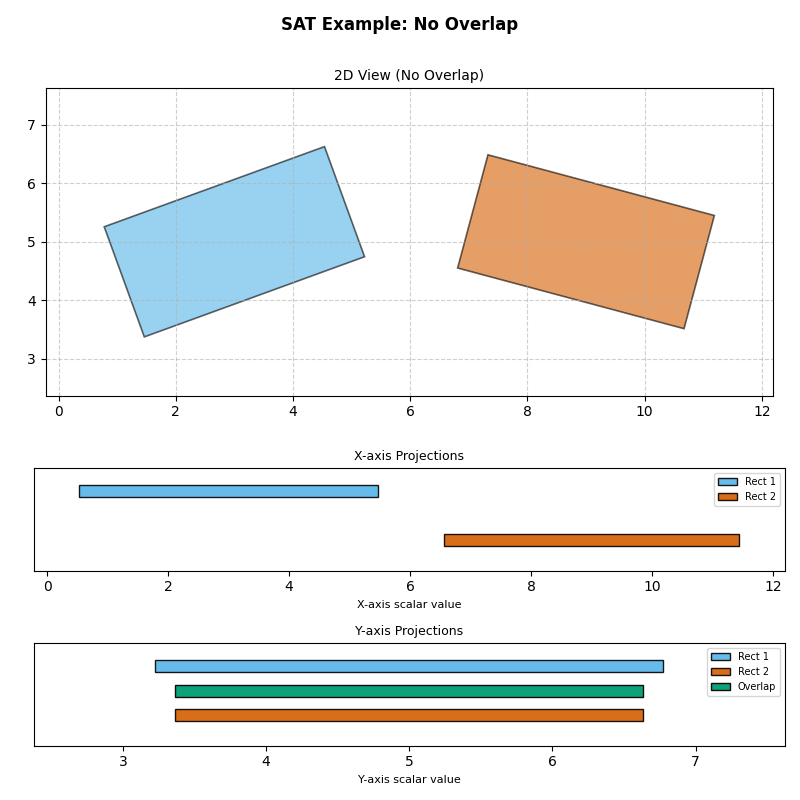
\includegraphics[width=\textwidth]{figures/sat_no_overlap_colored.png}
		\caption{Separation Axis Theorem with no overlap}
		\label{fig:1a_sat}
	\end{subfigure}
	\hfill
	\begin{subfigure}{0.45\textwidth}
		\centering
		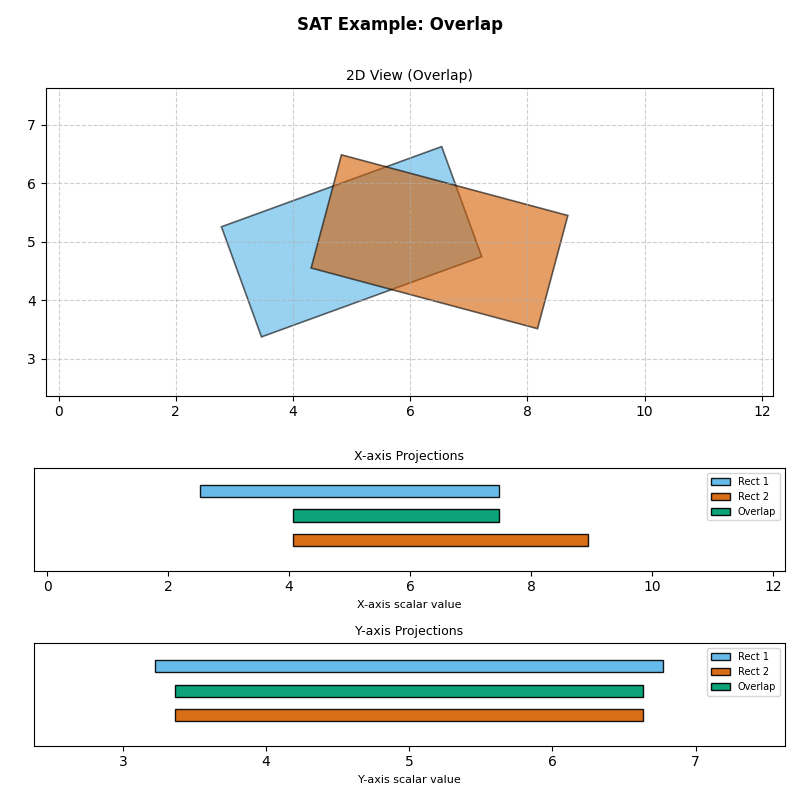
\includegraphics[width=\textwidth]{figures/sat_overlap_colored.png}
		\caption{Separation Axis Theorem with overlap}
		\label{fig:1b_sat}
	\end{subfigure}
	
	\caption{Separation Axis Theorem for oriented rectangles. Each figure consists of three subplots. The first subplot illustrates the spatial configuration of the rectangles. The second and third subplots show the projections of their principal axes onto the $x$- and $y$-axes, respectively. An overlap occurs when the projections intersect along both axes; the overlap is highlighted in black in the second and third subplots.}
	\label{fig:sat_theorem}
\end{figure}

During the search phase (lines~\ref{alg:start_pso_update}--\ref{alg:end_pso_update} of Algorithm~\ref{alg:pso_fixtures}), the velocity matrix $V_s$ and the position matrix $P_s$ associated with particle $s$ are iteratively updated according to the standard PSO update equations.

Whenever possible, constraint violations arising from updated fixture positions are mitigated through dedicated geometric repair procedures, as reported in lines~\ref{alg:start_fixing_geom}--\ref{alg:end_fixing_geom} of Algorithm~\ref{alg:pso_fixtures}. For each fixture, if its geometry lies partially or entirely outside the workpiece boundary, the nearest vertex of the workpiece polygon and the fixture vertex farthest from it are identified. The fixture is then translated by the minimum displacement required to satisfy the boundary constraint. The geometric repair strategy is limited to boundary violations, as these constraints are the most suitable for correction without adversely affecting the satisfaction of other constraints.

Lines~\ref{alg:start_fixing_type}--\ref{alg:end_fixing_type} of Algorithm~\ref{alg:pso_fixtures} report another constraints reparation strategy, where fixtures with type zero, representing unused fixtures, are directly assigned with the dummy lower-left corner coordinates $(\wtab,\htab)$, as in the CP model formulation (see Section~\ref{sec:second_cp_cons}), and are excluded from constraint violation evaluations.

To guide the search toward feasible positions, as illustrated in lines~\ref{alg:start_deb_eval}--\ref{alg:end_deb_eval} of Algorithm~\ref{alg:pso_fixtures}, candidate solutions are evaluated using Deb’s rules~\cite{deb2000efficient}:
\begin{itemize}
	\item Between two feasible solutions, retain the one with the higher objective value.
	\item Between a feasible and an infeasible solution, retain the feasible one.
	\item Between two infeasible solutions, retain the one with the lower constraint violation.
\end{itemize}

After updating the personal best position $P^*_s$ of each particle $s$ using Deb’s rules, the global best position $P^*$ of the swarm is updated accordingly. At the end of the final iteration, the best position found by the swarm is returned.


\section{Evaluation}
\label{sec:evaluation}
We evaluated the proposed resolution strategy on seven distinct workpieces: a stair step of a spiral staircase, a stair step of a simple staircase, a music speaker, a dashboard, a coffee table, a door, and a door with a porthole (see Table~\ref{tab:visual_results_first} and Table~\ref{tab:visual_results_second}).

The work center considered was equipped with 24 square fixtures with dimensions $145 \times 145$~mm and 12 rectangular fixtures with dimensions $180 \times 65$~mm. The minimum and maximum numbers of fixtures were set to $\nmin = 3$ and $\nmax = 6$, respectively, for all workpieces except the coffee table and the two door workpieces, which, due to their larger dimensions, required $\nmin = 6$ and $\nmax = 10$, and $\nmin = 10$ and $\nmax = 20$, respectively.

Both the CP and MIP models were implemented in MiniZinc version~2.9.5~\cite{nethercote2007minizinc}. The CP model was solved using the CP solvers Gecode~\cite{schulte2006gecode}, Chuffed~\cite{chuffed}, and OR-Tools~\cite{ortools}, whereas the MIP model was solved using the commercial solver Gurobi~\cite{gurobi}.

We also considered $\lns$, a variant of Gecode implementing Large Neighborhood Search (LNS)~\cite{pisinger2018large}, to solve the CP model, configuring it to explore the search space by randomly fixing 80\% of the decision variables corresponding to the $x$- and $y$-coordinates, adopting a constant restart strategy triggered every 1000 explored nodes.

All solvers were executed in single-threaded mode to ensure a fair comparison. The experiments were performed on a 64-bit Windows machine equipped with an Intel Core i5 processor and 16~GB of RAM.

Table~\ref{tab:objective_runtime} reports the values obtained for the objective function $\fdistarea$ for the different workpieces, together with the corresponding \emph{a posteriori} values of $\finer$, and the solve time $t_{solve}$ required to reach the optimal solution. 

Identical values of $\fdistarea$ do not necessarily correspond to identical values of $\finer$, as observed for the Dashboard workpiece. This is because the moments of inertia are highly sensitive to little displacement; therefore, if the solutions obtained by the solvers do not result in identical fixture placements, the value of $\finer$ may differ. 

Among the CP solvers, Gecode delivers the best overall performance, finding feasible solutions for all the considered workpieces, whereas Chuffed and OR-Tools fail to find feasible solutions for the two door workpieces.

$\lns$ achieves the best results for the two door workpieces, producing layouts that outperform those obtained by Gurobi with the MIP model. For the remaining workpieces, however, Gurobi finds solutions that are either superior or equivalent to those obtained by the CP solvers with respect to $\fdistarea$. This can be partly attributed to the use of continuous decision variables in the MIP model, which enlarges the feasible region and may therefore yield higher-quality solutions.

If we consider the information of the solve time presented in Table~\ref{tab:objective_runtime}, among the CP solvers, with an imposed time limit of 300~s, Chuffed is the most robust, finding the optimal solution in four of the seven instances, and it is the only CP solver able to prove optimality for the stiar step of the simple staircase. Gecode exhibits the greatest variability in performance, ranging from competitive runtimes on the easier instances to requiring 165.018~s for the speaker workpiece, while Chuffed and OR-Tools solve the same instance in only 0.106~s and 0.120~s, respectively.

Being a local-search-based approach, $\lns$ cannot prove optimality. Nevertheless, it reaches the same optimal value of $\fdistarea$ as the other CP solvers for the simpler workpieces and achieves the best value of $\finer$ in four out of the seven considered workpieces, demonstrating the effectiveness of a local search strategy.

\begin{landscape}
	
	\begin{table}[t]
		\centering
		\footnotesize
		\caption{Objective values for $\fdistarea$ and $\finer$, and solve time $t_{solve}$ in seconds to reach the best $\fdistarea$ solution. Timeout (300~s) is indicated by ``--''. Solutions where the solver reached optimality are marked with $^*$. For each workpiece, the maximum values of $\fdistarea$ and $\finer$ are highlighted in bold, including ties.}
		\label{tab:objective_runtime}
		\setlength{\tabcolsep}{2pt}
		\begin{tabular}{llccccc}
			\toprule
			Workpiece & Metric & Gecode & \lns & Chuffed & OR-Tools & Gurobi \\
			\midrule
			
			\multirow{3}{*}{\makecell{Stair step\\spiral staircase}} & $\fdistarea$ & $45655{}^*$ & $45655$ & $45655{}^*$ & $45655{}^*$ & $\mathbf{45662.155{}^*}$ \\
			& $\finer$ & \cellcolor{gray!15}$2.13968\times 10^{9}$ & \cellcolor{gray!15}$2.13968\times 10^{9}$ & \cellcolor{gray!15}$2.13960\times 10^{9}$ & \cellcolor{gray!15}$2.13968\times 10^{9}$ & \cellcolor{gray!15}$\mathbf{2.17089\times 10^{9}}$ \\
			& $t_{solve}$ & 0.559 & -- & 0.326 & 0.120 & 2.930 \\
			\midrule
			
			\multirow{3}{*}{\makecell{Stair step\\simple staircase}} & $\fdistarea$ & $72823$ & $72823$ & $72823{}^*$ & $72721$ & $\mathbf{72826.000{}^*}$ \\
			& $\finer$ & \cellcolor{gray!15}$6.76573\times 10^{9}$ & \cellcolor{gray!15}$6.76573\times 10^{9}$ & \cellcolor{gray!15}$6.76530\times 10^{9}$ & \cellcolor{gray!15}$6.48172\times 10^{9}$ & \cellcolor{gray!15}$\mathbf{6.76638\times 10^{9}}$ \\
			& $t_{solve}$ & -- & -- & 3.386 & -- & 0.220 \\
			\midrule
			
			\multirow{3}{*}{\makecell{Dashboard}} & $\fdistarea$ & $\mathbf{55582{}^*}$ & $\mathbf{55582}$ & $\mathbf{55582{}^*}$ & $\mathbf{55582{}^*}$ & $\mathbf{55582.000{}^*}$ \\
			& $\finer$ & \cellcolor{gray!15}$\mathbf{7.10094\times 10^{9}}$ & \cellcolor{gray!15}$\mathbf{7.10094\times 10^{9}}$ & \cellcolor{gray!15}$7.08735\times 10^{9}$ & \cellcolor{gray!15}$7.08735\times 10^{9}$ & \cellcolor{gray!15}$7.08735\times 10^{9}$ \\
			& $t_{solve}$ & 0.044 & -- & 0.057 & 0.102 & 0.157 \\
			\midrule
			
			\multirow{3}{*}{\makecell{Speaker}} & $\fdistarea$ & $\mathbf{49548{}^*}$ & $\mathbf{49548}$ & $\mathbf{49548{}^*}$ & $\mathbf{49548{}^*}$ & $\mathbf{49548.000{}^*}$ \\
			& $\finer$ & \cellcolor{gray!15}$\mathbf{2.93433\times 10^{9}}$ & \cellcolor{gray!15}$\mathbf{2.93433\times 10^{9}}$ & \cellcolor{gray!15}$\mathbf{2.93433\times 10^{9}}$ & \cellcolor{gray!15}$\mathbf{2.93433\times 10^{9}}$ & \cellcolor{gray!15}$\mathbf{2.93433\times 10^{9}}$ \\
			& $t_{solve}$ & 165.018 & -- & 0.106 & 0.120 & 0.126 \\
			\midrule
			
			\multirow{3}{*}{\makecell{Coffee table}} & $\fdistarea$ & $137262$ & $185351$ & $192711$ & $122920$ & $\mathbf{201686.505}$ \\
			& $\finer$ & \cellcolor{gray!15}$2.20750\times 10^{10}$ & \cellcolor{gray!15}$2.19967\times 10^{10}$ & \cellcolor{gray!15}$\mathbf{2.21449\times 10^{10}}$ & \cellcolor{gray!15}$9.10490\times 10^{9}$ & \cellcolor{gray!15}$2.19472\times 10^{10}$ \\
			& $t_{solve}$ & -- & -- & -- & -- & -- \\
			\midrule
			
			\multirow{3}{*}{\makecell{Door}} & $\fdistarea$ & $261757$ & $\mathbf{521632}$ & -- & -- & $355744.000$ \\
			& $\finer$ & \cellcolor{gray!15}$1.08442\times 10^{11}$ & \cellcolor{gray!15}$\mathbf{1.52925\times 10^{11}}$ & \cellcolor{gray!15}-- & \cellcolor{gray!15}-- & \cellcolor{gray!15}$1.17690\times 10^{11}$ \\
			& $t_{solve}$ & -- & -- & -- & -- & -- \\
			\midrule
			
			\multirow{3}{*}{\makecell{Door\\with porthole}} & $\fdistarea$ & $261759$ & $\mathbf{393343}$ & -- & -- & $298186.000$ \\
			& $\finer$ & \cellcolor{gray!15}$1.08422\times 10^{11}$ & \cellcolor{gray!15}$\mathbf{1.52861\times 10^{11}}$ & \cellcolor{gray!15}-- & \cellcolor{gray!15}-- & \cellcolor{gray!15}$1.39714\times 10^{11}$ \\
			& $t_{solve}$ & -- & -- & -- & -- & -- \\
			
			\bottomrule
		\end{tabular}
	\end{table}
	
\end{landscape}

The Q-learning based algorithm was implemented in Python~3.11.9 using the Gymnasium library version~1.3.0. The agent was trained on all the considered workpieces for 200 episodes, each consisting of 20 steps, using the following hyperparameters: learning rate $\alpha = 0.1$, discount factor $\gamma = 0.99$, initial exploration rate $\epsilon = 1.0$, and exploration decay factor $\rho = 0.995$.

Table~\ref{tab:comparison} reports the results obtained for the different workpieces, comparing the corresponding values of the moment of inertia with those achieved by the best CP solver and the MIP model.

Overall, the Q-learning based algorithm does not outperform either the CP or the MIP model. On average, the values of $\finer$ obtained by Q-learning are 13\% lower than those achieved by CP and 8\% lower than those obtained with MIP. The only exception is the door with a porthole workpiece, for which Q-learning outperforms the solution returned by Gurobi for the MIP model.


\begin{table}[t]
	\centering
	\footnotesize
	\caption{Objective values $\finer$ comparison: CP solvers (best among Gecode, LNS, Chuffed, OR-Tools), MIP solver (Gurobi), and RL approach. For each workpiece, the maximum value is highlighted in bold.}
	\label{tab:comparison}
	\setlength{\tabcolsep}{5pt}
	\begin{tabular}{cccc}
		\toprule
		Workpiece & CP model & MIP model & Q-learning \\
		\midrule
		
		\makecell{Stair step\\spiral staircase} & $2.13968\times 10^{9}$ & $\mathbf{2.17089\times 10^{9}}$ & $1.93822\times 10^{9}$ \\
		\midrule
		
		\makecell{Stair step\\simple staircase} & $6.76573\times 10^{9}$ & $\mathbf{6.76638\times 10^{9}}$ & $5.65433\times 10^{9}$ \\
		\midrule
		
		\makecell{Dashboard} & $\mathbf{7.10094\times 10^{9}}$ & $7.08735\times 10^{9}$ & $6.65446\times 10^{9}$ \\
		\midrule
		
		\makecell{Speaker} & $\mathbf{2.93433\times 10^{9}}$ & $\mathbf{2.93433\times 10^{9}}$ & $2.81248\times 10^{9}$ \\
		\midrule
		
		\makecell{Coffee table} & $\mathbf{2.29750\times 10^{10}}$ & $2.19472\times 10^{10}$ & $1.56444\times 10^{10}$ \\
		\midrule
		
		\makecell{Door} & $\mathbf{1.52925\times 10^{11}}$ & $1.17690\times 10^{11}$ & $1.14387\times 10^{11}$ \\
		\midrule
		
		\makecell{Door\\with porthole} & $\mathbf{1.52861\times 10^{11}}$ & $1.39714\times 10^{11}$ & $1.45467\times 10^{11}$ \\
		
		\bottomrule
	\end{tabular}
\end{table}


\begin{figure}[t]
	\centering
	\begin{subfigure}[b]{\textwidth}
		\centering
		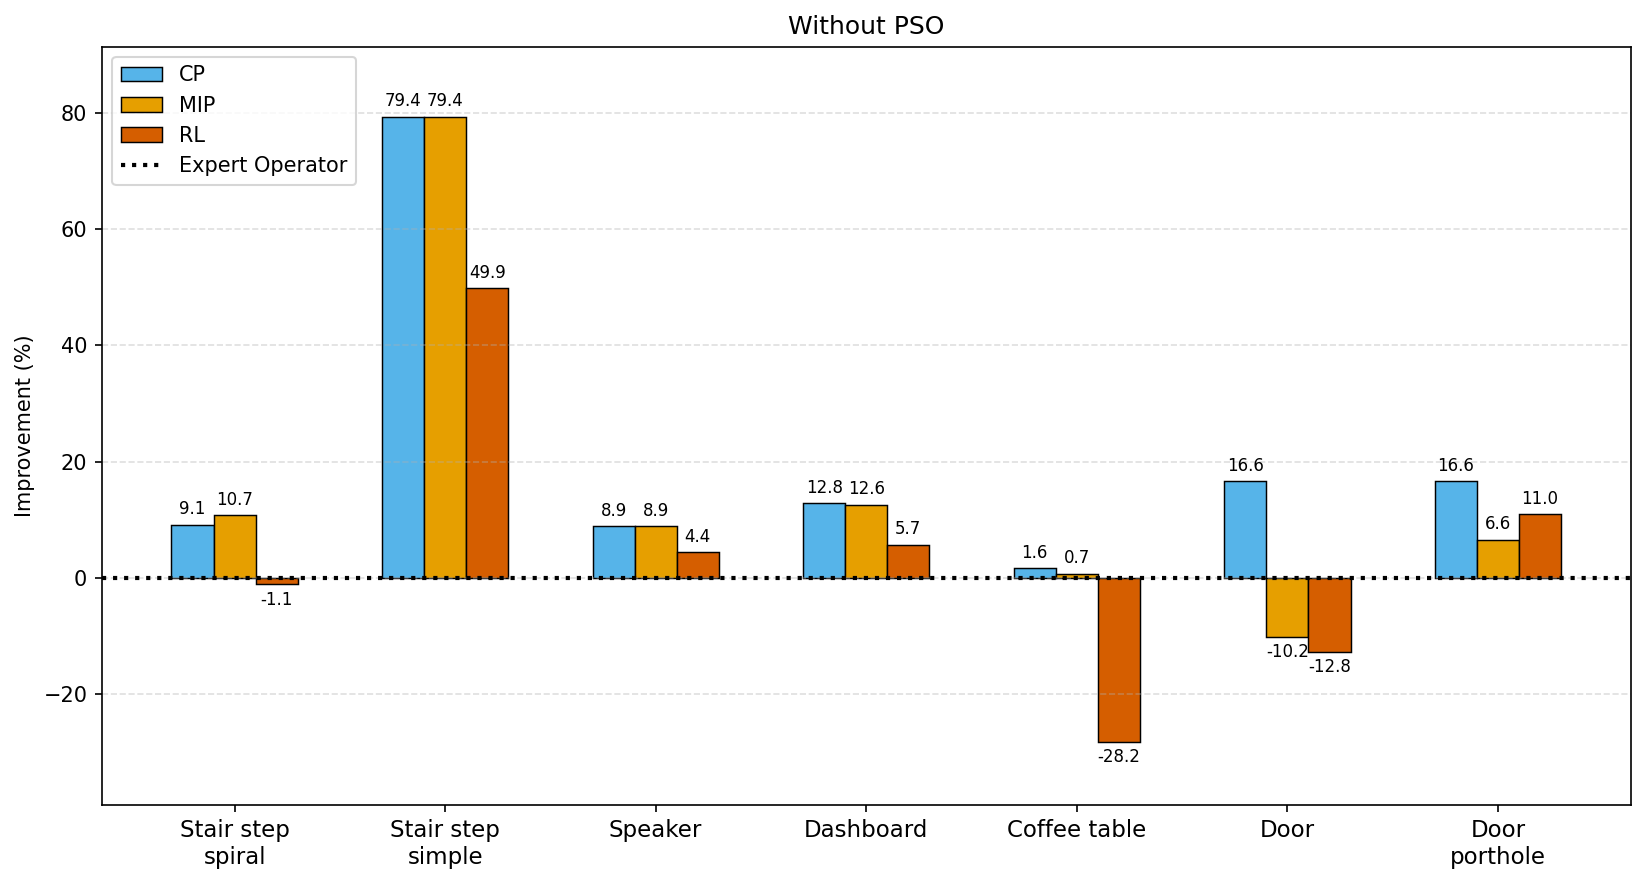
\includegraphics[width=\textwidth]{figures/comparison_plot_1.png}
		\caption{Percentage improvement over expert operator}
		\label{fig:comparison_plot1}
	\end{subfigure}
	%\hspace{1.5cm}
	\begin{subfigure}[b]{\textwidth}
		\centering
		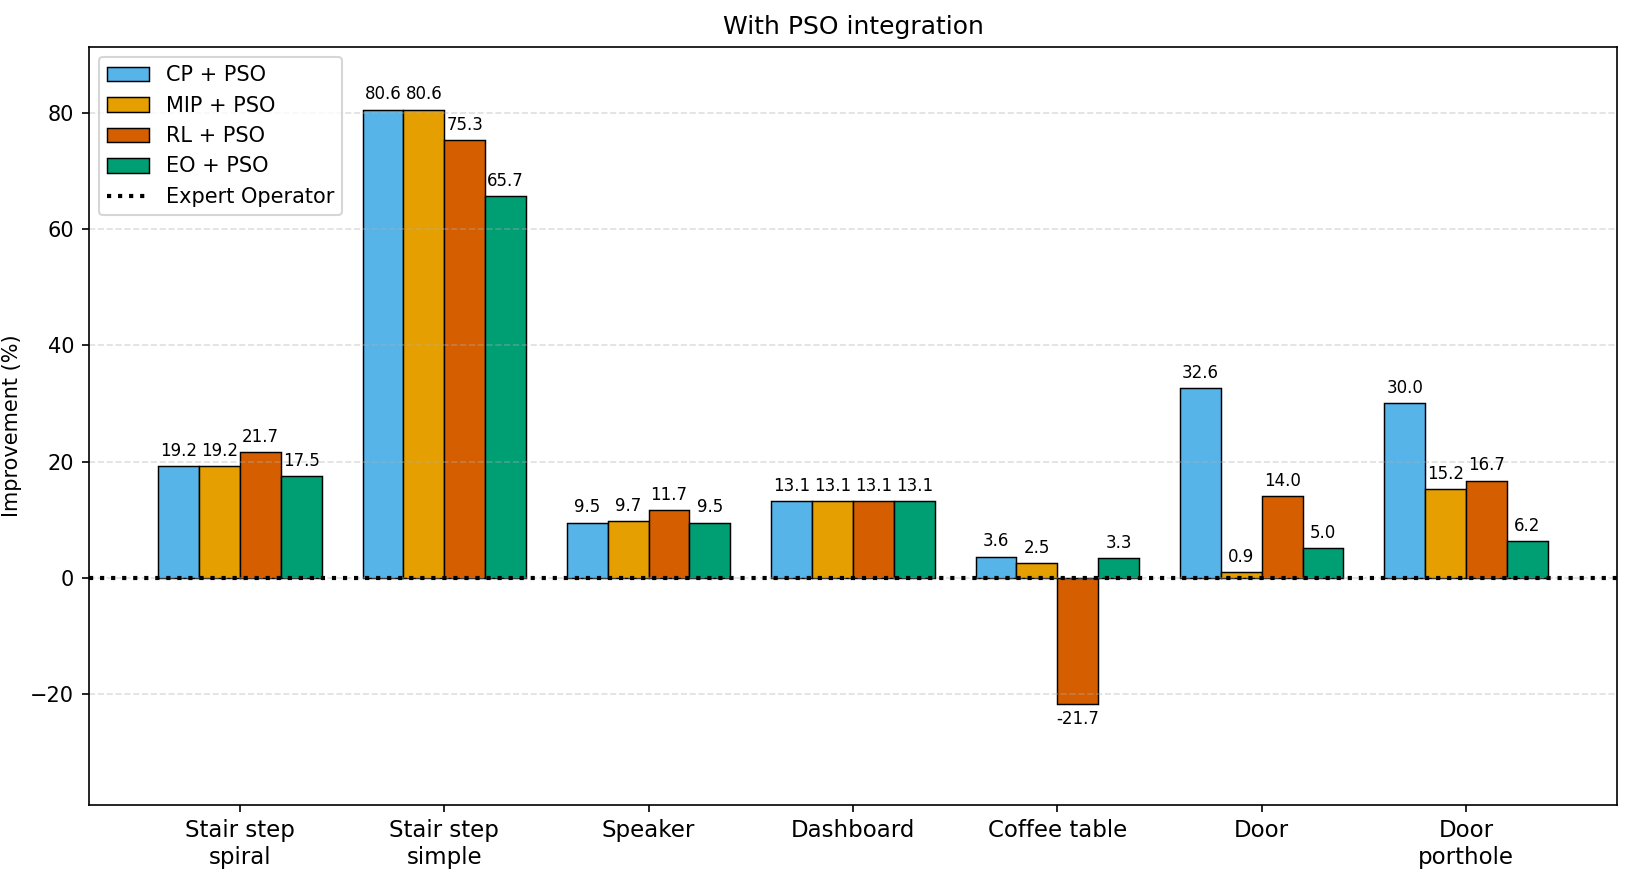
\includegraphics[width=\textwidth]{figures/comparison_plot_2.png}
		\caption{Percentage improvement over expert operator after PSO refinement}
		\label{fig:comparison_plot2}
	\end{subfigure}
	\caption{Percentage improvement relative to the solution provided by the expert operator. The first plot illustrates the improvements achieved by the CP model, MIP model and Q-learning algorithm without PSO integration, whereas the second plot presents the improvements obtained with PSO integration, alongside the improvement of the expert operator's solution when combined with PSO.}
	\label{fig:improvement}
\end{figure}

For each workpiece, the best CP and MIP solutions in terms of $\finer$, together with the Q-learning solution, were used as initial ones for the PSO algorithm. 

To enable direct integration into the target industrial system, the PSO algorithm was implemented in Java~18.0.2. Its hyper-parameters were tuned using the Optuna framework~\cite{akiba2019optuna}, yielding the following configuration: $\swarmsize = 1374$, $\maxiter = 2912$, $w = 0.669$, $c_1 = 2.385$, and $c_2 = 0.558$.

Figure~\ref{fig:improvement} shows the percentage improvement in $\finer$ with respect to the layout proposed by an expert operator. The first plot (Figure~\ref{fig:comparison_plot1}) reports the improvements achieved by the CP model, the MIP model, and the Q-learning algorithm before PSO refinement, whereas the second plot (Figure~\ref{fig:comparison_plot2}) shows the corresponding results after PSO refinement, including those obtained by initializing PSO from the expert layout.

The largest workpieces, namely the coffee table, the door, and the door with porthole, represent the most challenging instances. Among the considered approaches, the CP model consistently achieves the best improvements over the expert layout and is the only one that improves upon the expert solution for the door workpiece.

The Q-learning algorithm outperforms the expert layout in four of the seven considered workpieces. The integration with PSO further improves the solutions generated by the Q-learning algorithm for the stair step of the spiral staircase and the door, allowing them to surpass the expert layout. Conversely, when initialized with the Q-learning solution for the Coffee table, which represents the weakest initial layout, PSO achieves only marginal improvements, highlighting the importance of providing a high-quality starting solution.

The plot in Figure~\ref{fig:comparison_plot2} reports in green the improvement achieved by initializing PSO with the expert operator layout, and for all the considered workpieces, PSO generates layouts that outperform the expert solution, demonstrating its effectiveness as a refinement technique.

\begin{landscape}
	\begin{table}[t]
		\centering
		\renewcommand{\arraystretch}{1.3}
		\setlength{\tabcolsep}{3pt}
		\caption{Summary of the best solutions, corresponding solution providers, and moment of inertia values for the first four workpieces. 
			The workpiece perimeter is shown with solid lines. Dashed lines indicate areas to be extruded, fixture regions are marked with diagonal hatching, and supporting bars are shown as shaded rectangles.}
		\label{tab:visual_results_first}
		\begin{tabular}{c c c c c}
			\hline
			\textbf{Workpiece} & \textbf{Expert Operator} & \textbf{Best CP/MIP} & \textbf{Q-learning} & \textbf{Best with PSO} \\
			\hline
			
			\makecell{Spiral stair step} & 
			\makecell{$1.96057\times 10^{9}$ \\ 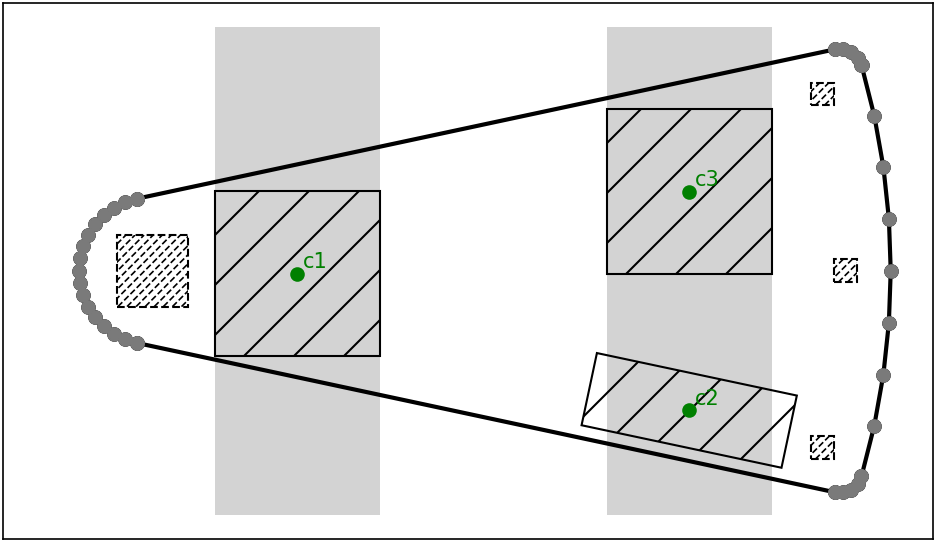
\includegraphics[width=0.18\linewidth]{figures/spiral_stair_step_expert_operator.png}} & 
			\makecell{MIP: $2.17089\times 10^{9}$ \\ 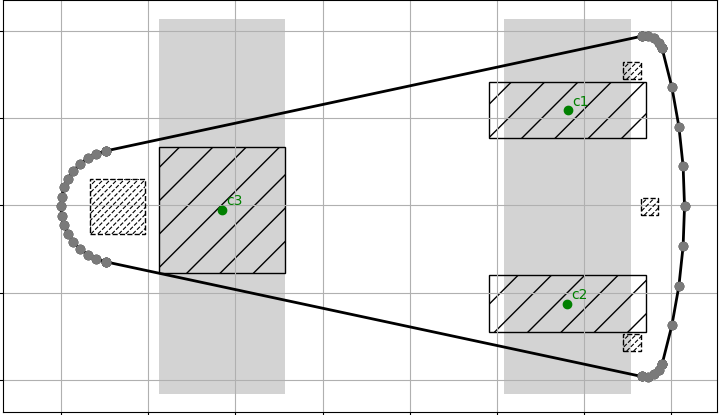
\includegraphics[width=0.18\linewidth]{figures/spiral_stair_step_mip_model_gurobi.png}} & 
			\makecell{$1.93822\times 10^{9}$ \\ 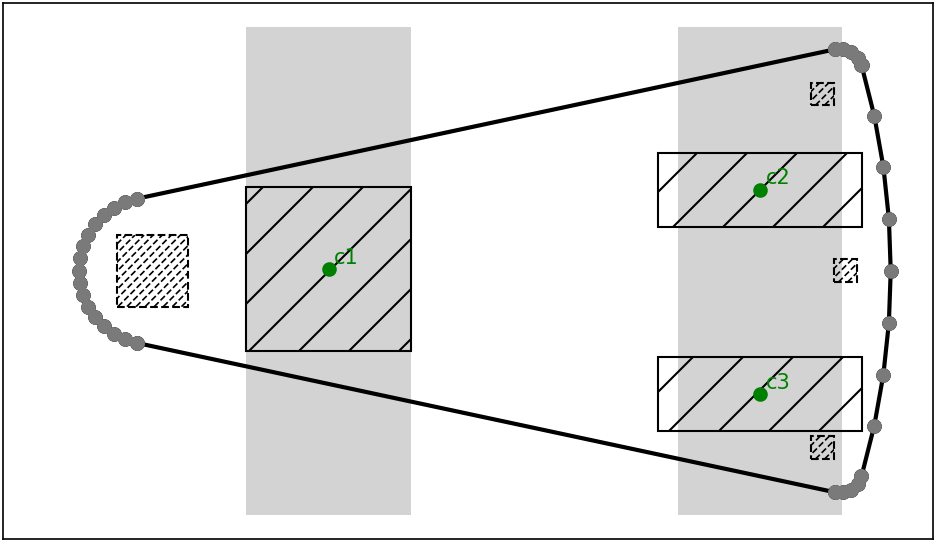
\includegraphics[width=0.18\linewidth]{figures/spiral_stair_step_rl.png}} & 
			\makecell{RL: $2.38520\times 10^{9}$ \\ 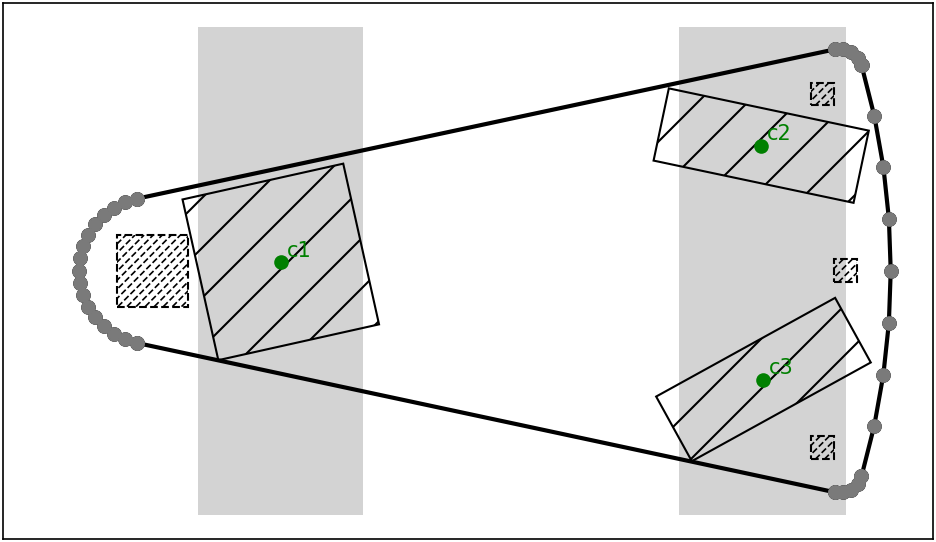
\includegraphics[width=0.18\linewidth]{figures/spiral_stair_step_pso_rl_pso.png}} \\
			\hline
			
			\makecell{Simple stair step} & 
			\makecell{$3.77213\times 10^{9}$ \\ 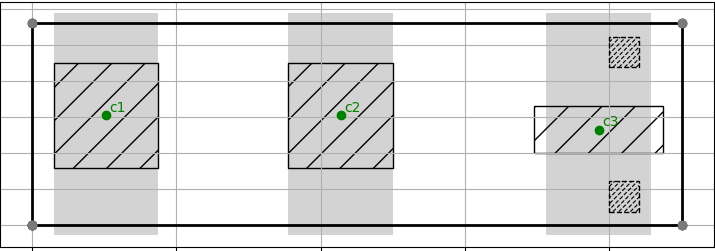
\includegraphics[width=0.18\linewidth]{figures/simple_stair_step_expert_operator.png}} & 
			\makecell{MIP: $6.76638\times 10^{9}$ \\ 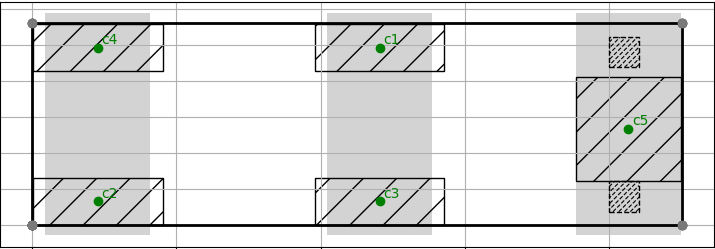
\includegraphics[width=0.18\linewidth]{figures/simple_stair_step_mip_model_gurobi.png}} & 
			\makecell{$5.65433\times 10^{9}$ \\ 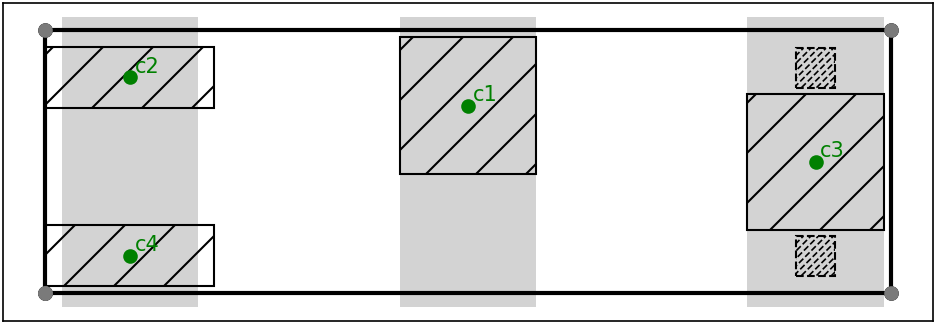
\includegraphics[width=0.18\linewidth]{figures/simple_stair_step_rl.png}} & 
			\makecell{CP: $6.81108\times 10^{9}$ \\ 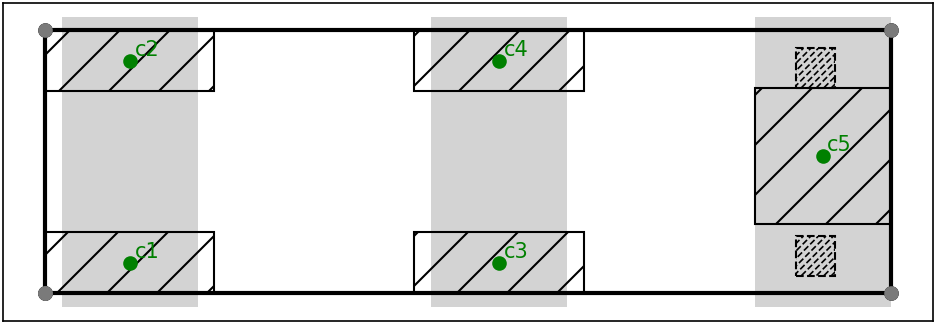
\includegraphics[width=0.18\linewidth]{figures/simple_stair_step_pso_cp_pso.png}} \\
			\hline
			
			\makecell{Dashboard} & 
			\makecell{$6.29544\times 10^{9}$ \\ 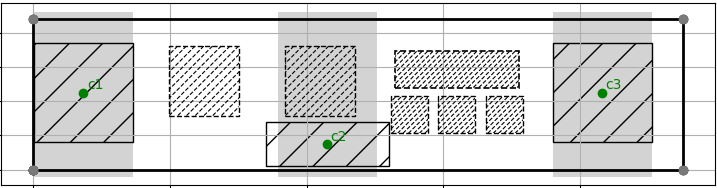
\includegraphics[width=0.18\linewidth]{figures/dashboard_expert_operator.png}} & 
			\makecell{CP: $7.10094\times 10^{9}$ \\ 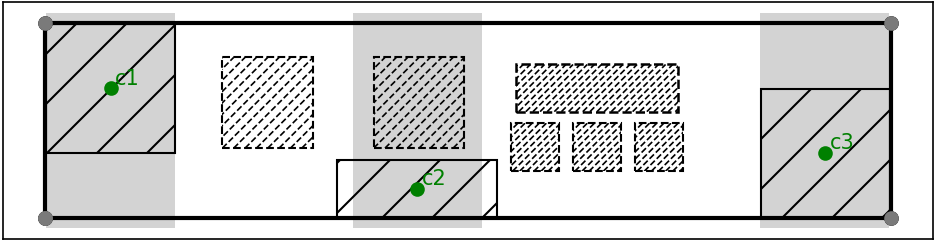
\includegraphics[width=0.18\linewidth]{figures/dashboard_cp_model_gecode.png}} & 
			\makecell{$6.65446\times 10^{9}$ \\ 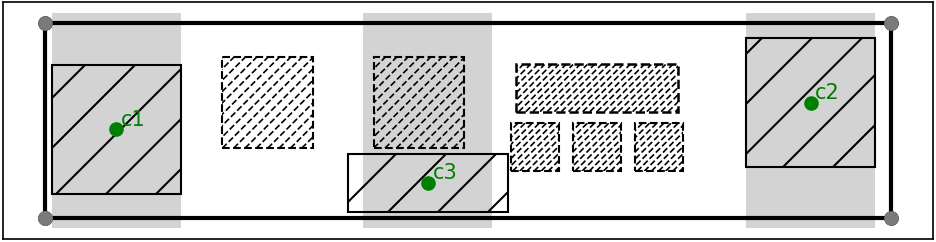
\includegraphics[width=0.18\linewidth]{figures/dashboard_rl.png}} & 
			\makecell{CP: $7.12226\times 10^{9}$ \\ 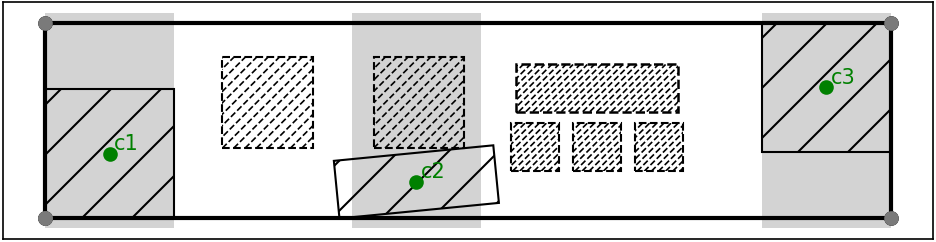
\includegraphics[width=0.18\linewidth]{figures/dashboard_pso_cp_pso.png}} \\
			\hline
			
			\makecell{Speaker} & 
			\makecell{$2.69490\times 10^{9}$ \\ 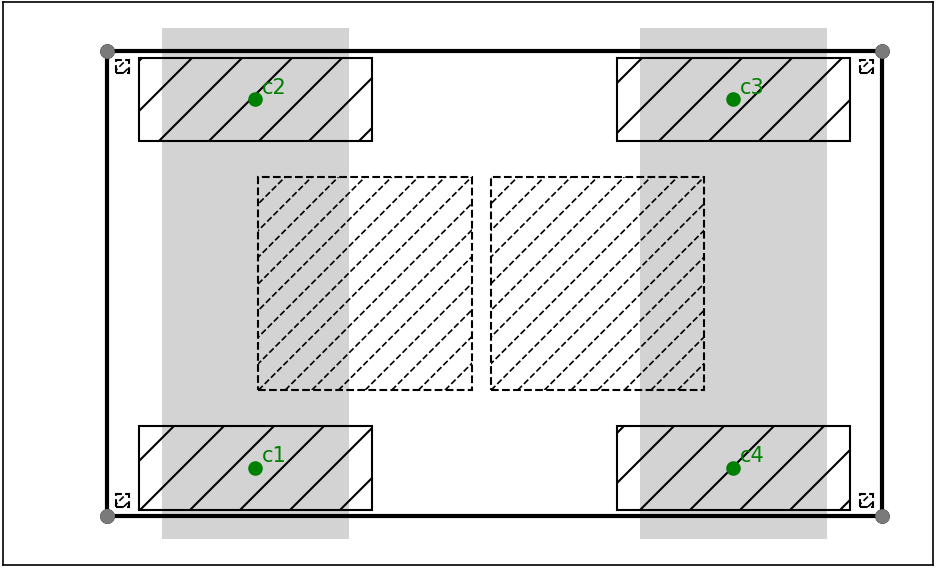
\includegraphics[width=0.18\linewidth]{figures/speaker_expert_operator.png}} & 
			\makecell{CP, MIP: $2.93433\times 10^{9}$ \\ 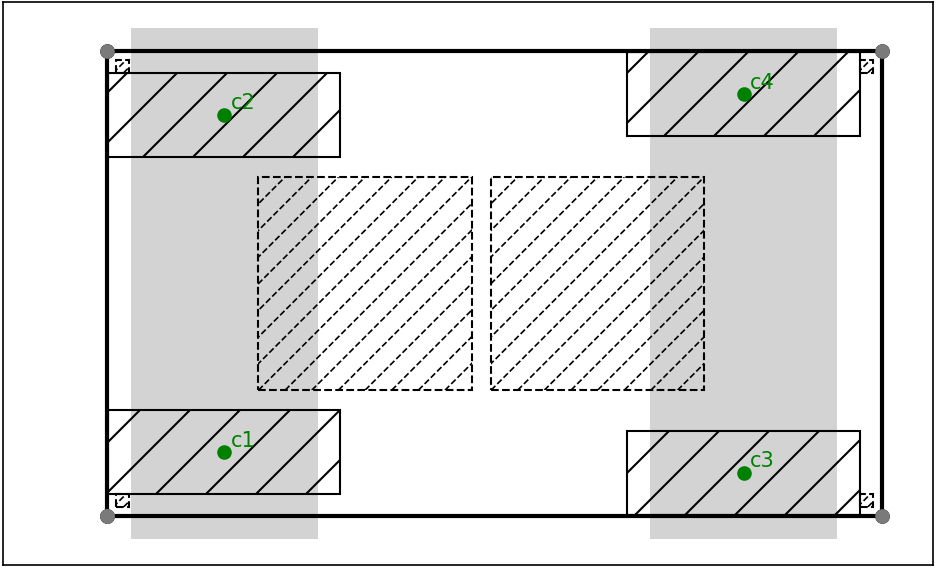
\includegraphics[width=0.18\linewidth]{figures/speaker_cp_model_gecode.png}} & 
			\makecell{$2.81248\times 10^{9}$ \\ 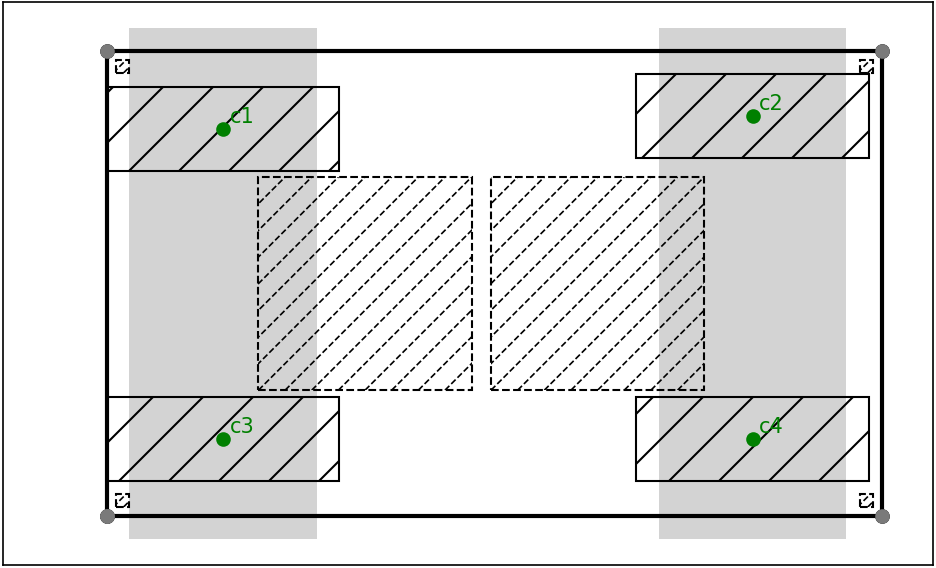
\includegraphics[width=0.18\linewidth]{figures/speaker_rl.png}} & 
			\makecell{RL: $3.00979\times 10^{9}$ \\ 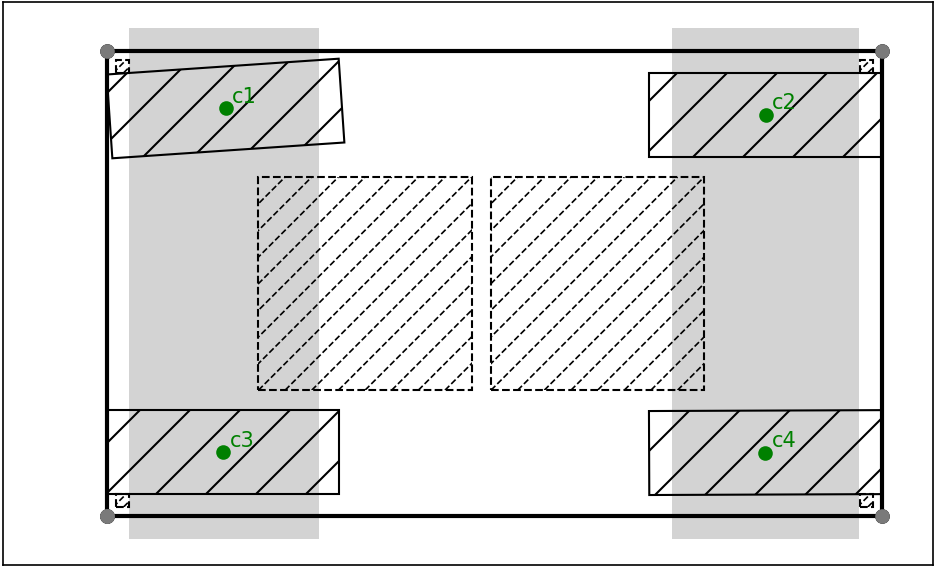
\includegraphics[width=0.18\linewidth]{figures/speaker_pso_rl_pso.png}} \\
			\hline
			
		\end{tabular}
	\end{table}
	
	\begin{table}[t]
		\centering
		\renewcommand{\arraystretch}{1.3}
		\setlength{\tabcolsep}{3pt}
		\caption{Summary of the best solutions, corresponding solution providers, and moment of inertia values for the remaining three workpieces. 
			The workpiece perimeter is shown with solid lines. Dashed lines indicate areas to be extruded, fixture regions are marked with diagonal hatching, and supporting bars are shown as shaded rectangles.}
		\label{tab:visual_results_second}
		\begin{tabular}{c c c c c}
			\hline
			\textbf{Workpiece} & \textbf{Expert Operator} & \textbf{Best CP/MIP} & \textbf{Q-learning} & \textbf{Best with PSO} \\
			\hline
			
			\makecell{Coffee table} & 
			\makecell{$2.17954\times 10^{10}$ \\ 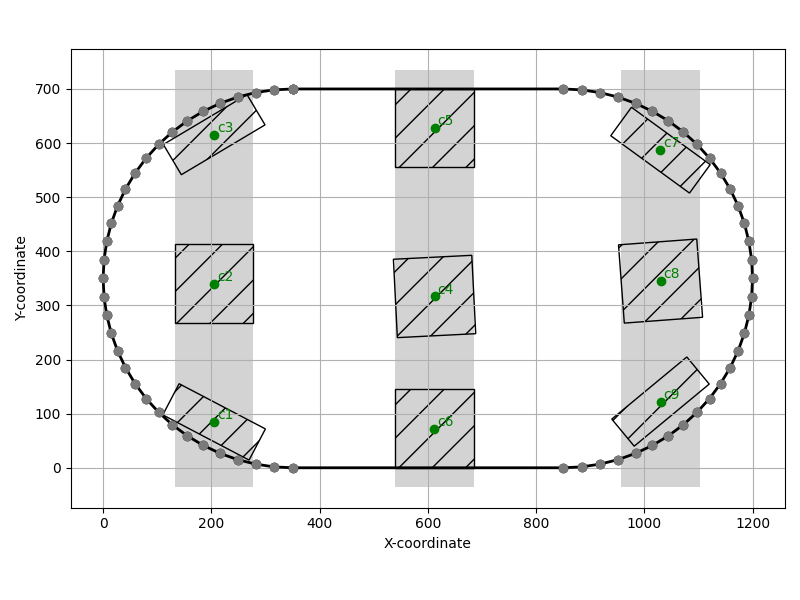
\includegraphics[width=0.18\linewidth]{figures/coffee_table_expert_operator.png}} & 
			\makecell{CP: $2.21449\times 10^{10}$ \\ 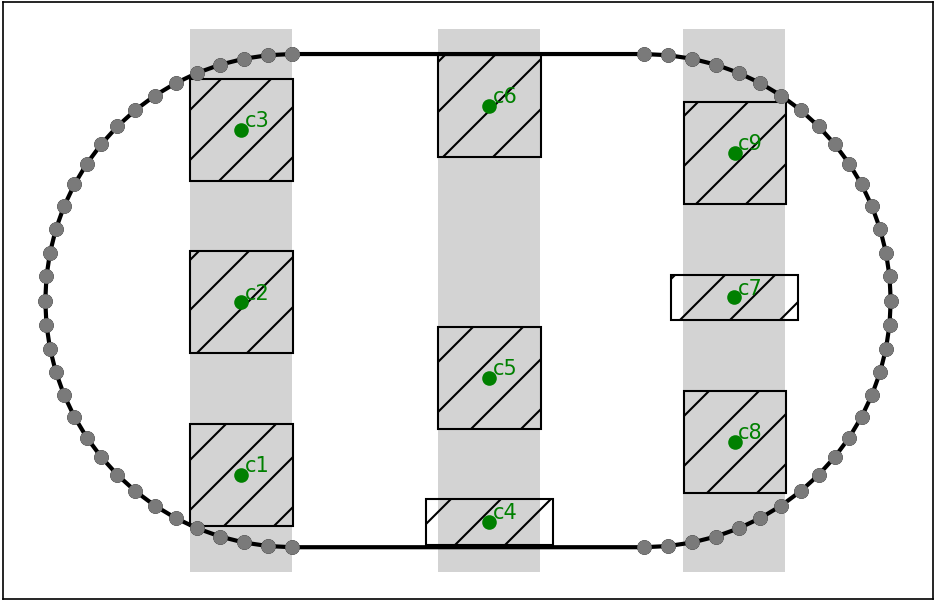
\includegraphics[width=0.18\linewidth]{figures/coffee_table_cp_model_chuffed.png}} & 
			\makecell{$1.56444\times 10^{10}$ \\ 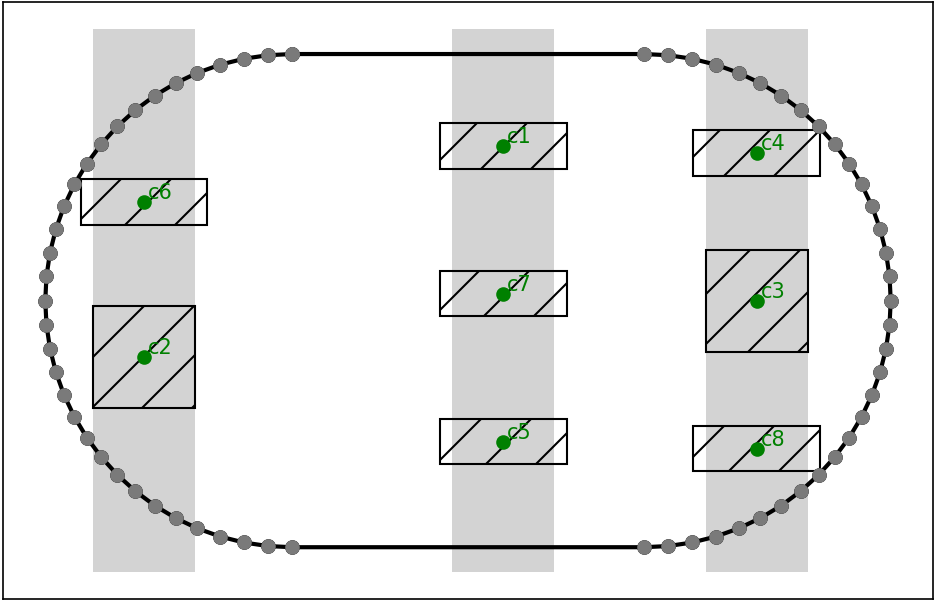
\includegraphics[width=0.18\linewidth]{figures/coffee_table_rl.png}} & 
			\makecell{CP: $2.25868\times 10^{10}$ \\ 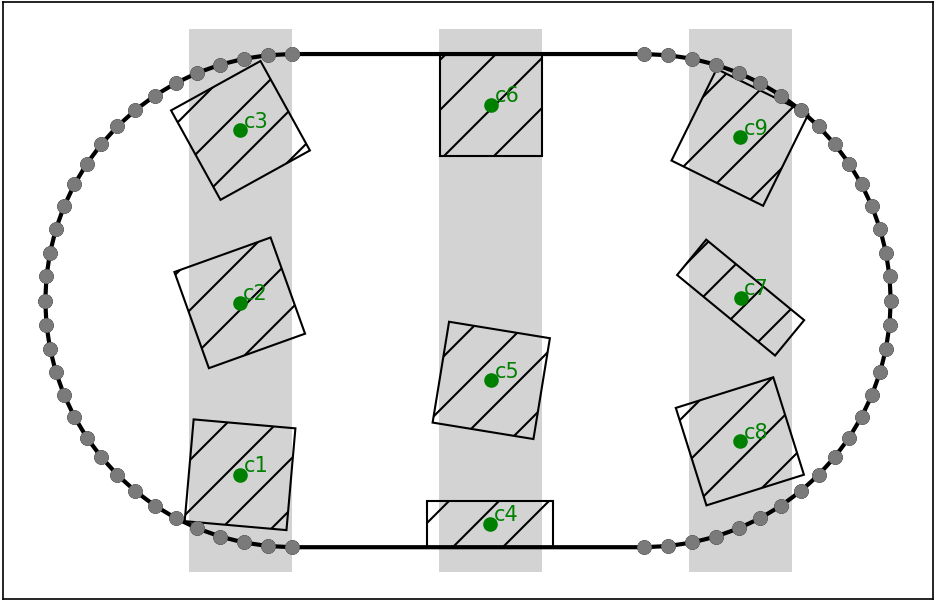
\includegraphics[width=0.18\linewidth]{figures/coffee_table_pso_cp_pso.png}} \\
			\hline
			
			\makecell{Door} & 
			\makecell{$1.31109\times 10^{11}$ \\ 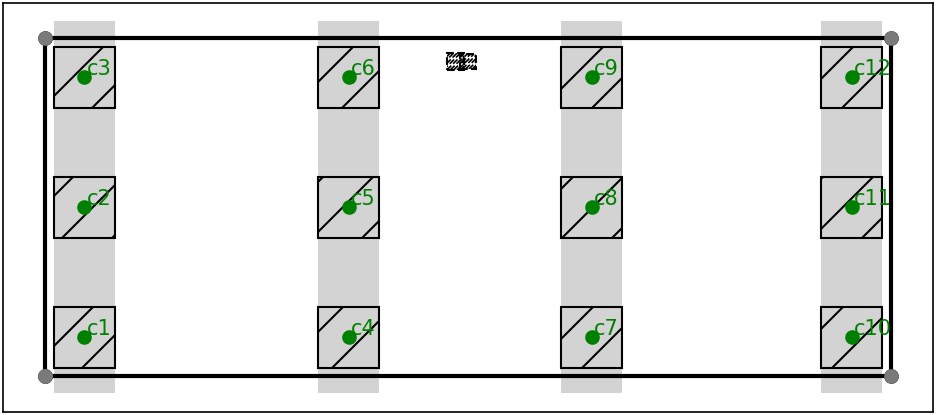
\includegraphics[width=0.18\linewidth]{figures/door_expert_operator.png}} & 
			\makecell{CP: $1.52925\times 10^{11}$ \\ 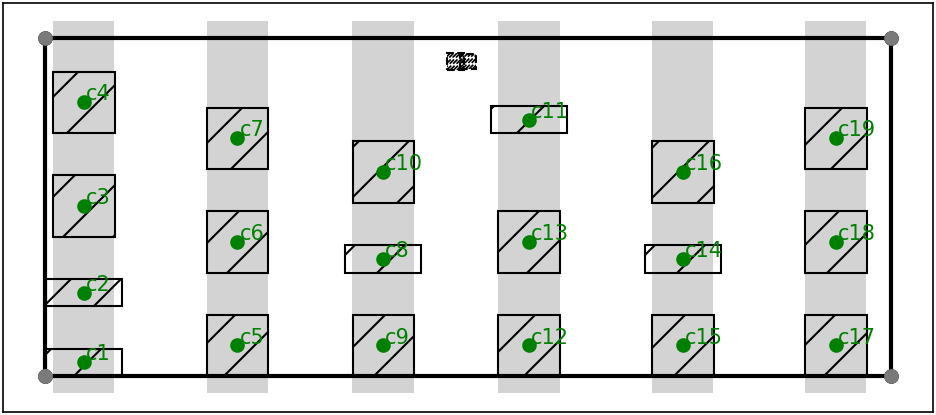
\includegraphics[width=0.18\linewidth]{figures/door_LNS_cp_model_gecode.png}} & 
			\makecell{$1.14387\times 10^{11}$ \\ 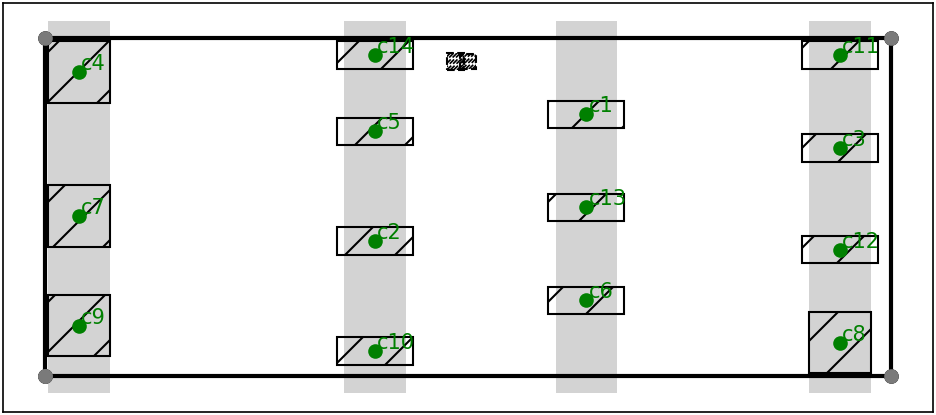
\includegraphics[width=0.18\linewidth]{figures/door_rl.png}} & 
			\makecell{CP: $1.73826\times 10^{11}$ \\ 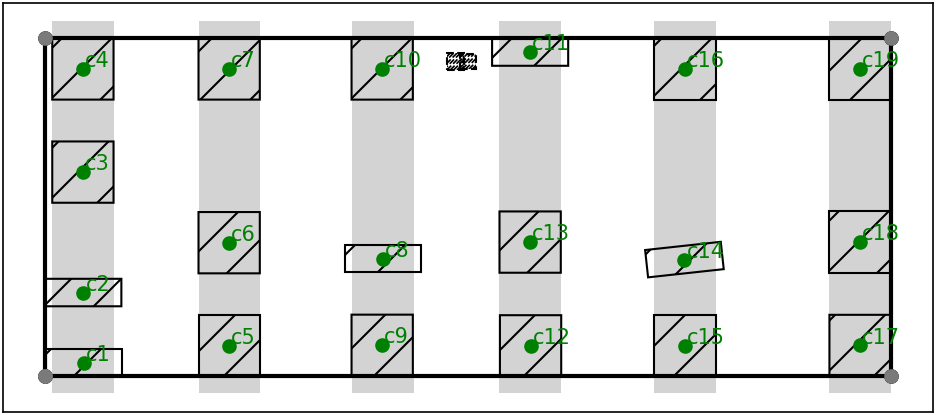
\includegraphics[width=0.18\linewidth]{figures/door_pso_cp_pso.png}} \\
			\hline
			
			\makecell{Door porthole} & 
			\makecell{$1.31109\times 10^{11}$ \\ 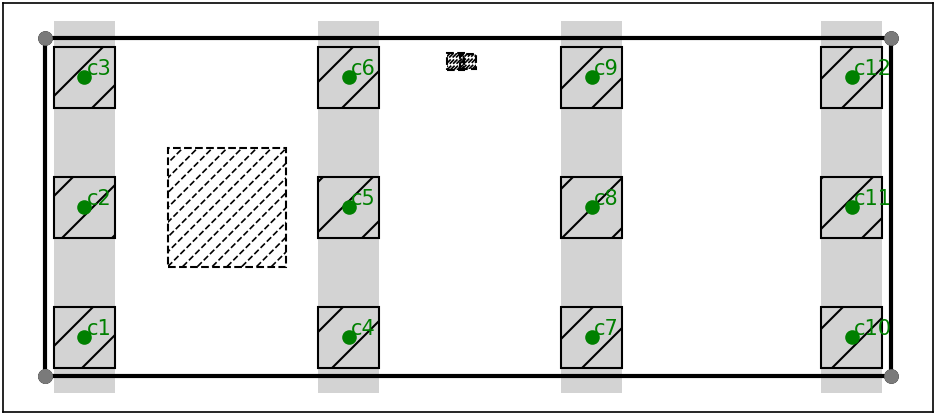
\includegraphics[width=0.18\linewidth]{figures/door_porthole_expert_operator.png}} & 
			\makecell{CP: $1.52861\times 10^{11}$ \\ 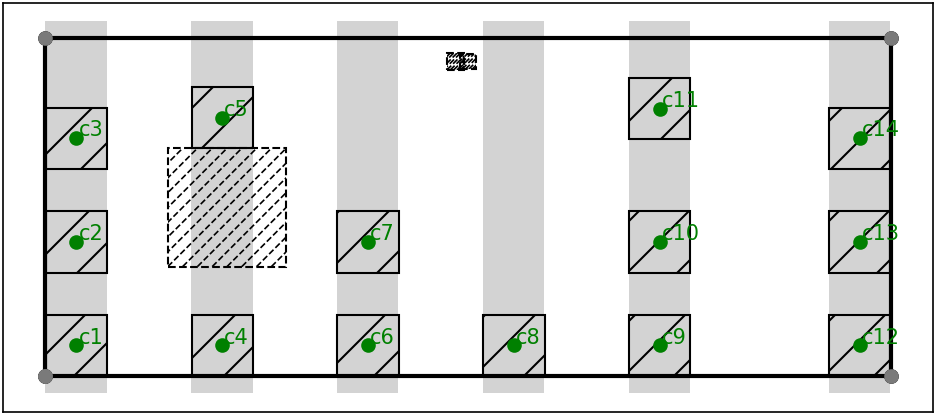
\includegraphics[width=0.18\linewidth]{figures/door_porthole_LNS_cp_model_gecode.png}} & 
			\makecell{$1.45467\times 10^{11}$ \\ 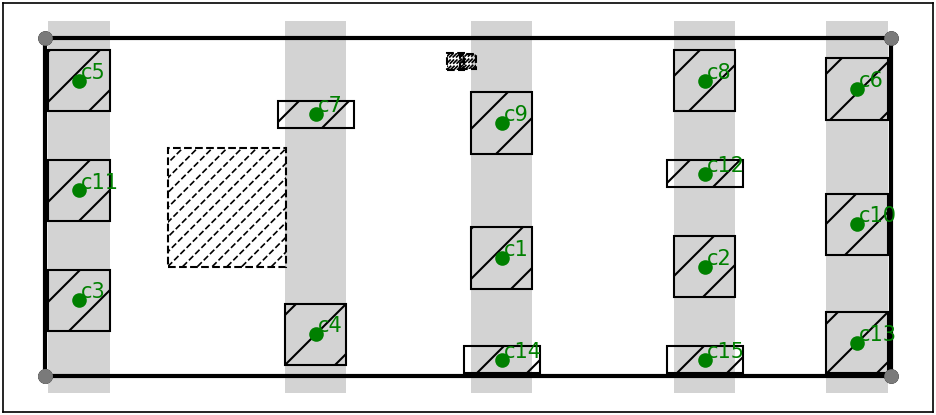
\includegraphics[width=0.18\linewidth]{figures/door_porthole_rl.png}} & 
			\makecell{CP: $1.70507\times 10^{11}$ \\ 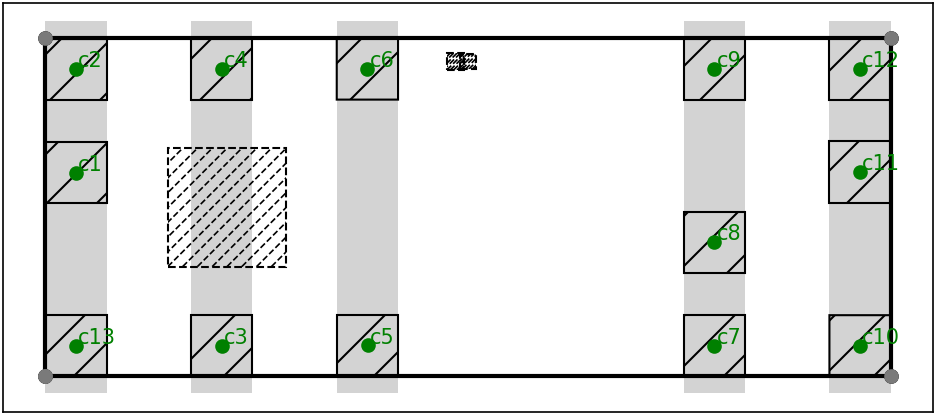
\includegraphics[width=0.18\linewidth]{figures/door_porthole_pso_cp_pso.png}} \\
			\hline
			
		\end{tabular}
	\end{table}
\end{landscape}

Tables~\ref{tab:visual_results_first} and ~\ref{tab:visual_results_second} report visual comparisons of the best solutions obtained with the CP model, the MIP model, and the Q-learning algorithm for the different workpieces, together with the corresponding solutions refined by PSO. Note that, in the figures, the support bars can be positioned beneath the areas to be extruded, since the fixture height prevents collisions between the cutting tools and the bars.

The layouts proposed by the Q-learning algorithm are qualitatively similar to those obtained with the CP and MIP models. An exception is the coffee table, where Q-learning tends to favour the placement of a larger number of rectangular fixtures instead of square ones, resulting in a lower value for the moment of inertia.

Rotation plays an important role in the stair step of the spiral staircase and coffee table workpieces, where fixture orientation improves adherence to the workpiece boundary. For the Speaker workpiece, the PSO refinement of the Q-learning solution introduces only a slight rotation of the upper-left fixture, yielding the marginal improvement reported in Figure~\ref{fig:improvement}.

The stair step of the simple staircase exhibits the largest improvement over the expert layout. This is mainly due to the use of a larger number of fixtures, five for the CP and MIP models and four for the Q-learning algorithm, compared with the three fixtures used by the expert operator.

For both the door and the door with a porthole workpieces, the expert operator adopts a symmetric fixture layout, whereas the PSO refinement tends to move the fixtures farther from the workpiece centre. Since the principal moments of inertia are maximised when the fixtures are placed away from the symmetry axes, this configuration yields higher values of $\finer$. Moreover, in the door workpiece, the expert layout relies exclusively on square fixtures, whereas the optimization strategies increase the number of fixtures using even rectangular ones, thereby increasing the supported area of the workpiece.

Overall, the best trade-off between computational time and solution quality is achieved by integrating the CP model with PSO. The CP formulation is expected to scale better to problems involving additional fixture types and multiple areas to be extruded owing to the stronger propagation of the \texttt{diffn} global constraint and the fact that type and overlap decisions are modeled through discrete variables that cannot be relaxed, unlike the $x$ and $y$ variables in the MIP formulation.



	
	\chapter{FlatZinc based Particle Swarm Optimization}
	\label{chap:pt1_chapter7}

In Section~\ref{sec:pso_algorithm}, we stated that the linear constraints of the MIP model were used as a reference to model the constraints in PSO and incorporated into its implementation to evaluate the feasibility of the layouts. 

Implementing this approach, however, requires the MIP constraints to be reformulated into a form that can be evaluated by PSO. Since the MIP model was developed in MiniZinc, this reformulation can be avoided by exploiting the FlatZinc file generated during model compilation. The constraint evaluation performed by PSO can then be based directly on the information contained in this file.

This chapter presents the implementation of this solution through the development of a FlatZinc-based PSO algorithm designed to solve MiniZinc models involving continuous variables and nonlinear constraints. Before describing the algorithm in detail, the following sections discuss the structure of the FlatZinc model and how it is represented within the FlatZinc-based PSO.


\section{FlatZinc model and flattening process}
\label{sec:flattening}

The process of converting a MiniZinc model into a FlatZinc model is known as \emph{flattening}. During this process, the variables of the original model are retained, arrays of variables are expanded into indexed variables, and constraints are rewritten into a primitive form supported by the target solver. Listing~\ref{lst:json_example} illustrates this process by presenting the FlatZinc model generated from the MiniZinc model presented in Listing~\ref{lst:minizinc_example}.

\begin{lstlisting}[language=MiniZinc, caption={Example of MiniZinc model}, label={lst:minizinc_example}]
	var -1.0..1.0: x1;
	var -1.0..1.0: x2;
	
	var float: objective =
	pow(x1, 2.0) + pow(x2 - 1.0, 2.0);
	
	constraint x2 - pow(x1, 2.0) = 0.0;
	
	solve minimize objective;
\end{lstlisting}

\begin{lstlisting}[language=json, caption={JSON representation of the FlatZinc model}, label={lst:json_example}]
	{
		"variables": {
			"x1" : { "type" : "float", "domain" : [[-1.0, 1.0]] },
			"x2" : { "type" : "float", "domain" : [[-1.0, 1.0]], "defined" : true },
			"objective" : { "type" : "float", "defined" : true },
			"X_INTRODUCED_1_" : { "type" : "float", "domain" : [[-2.0, 0.0]], "introduced": true, "defined" : true },
			"X_INTRODUCED_2_" : { "type" : "float", "introduced": true, "defined" : true }
		},
		"arrays": {
		},
		"constraints": [
		{ "id" : "float_pow", "args" : ["X_INTRODUCED_1_", 2.0, "X_INTRODUCED_2_"], "defines" : "X_INTRODUCED_2_"},
		{ "id" : "float_pow", "args" : ["x1", 2.0, "x2"], "defines" : "x2"},
		{ "id" : "float_lin_eq", "args" : [[1.0, 1.0, -1.0], ["x2", "X_INTRODUCED_2_", "objective"], -0.0], "defines" : "objective"},
		{ "id" : "float_lin_eq", "args" : [[1.0, -1.0], ["x2", "X_INTRODUCED_1_"], 1.0], "defines" : "X_INTRODUCED_1_"}
		],
		"output": ["x1", "x2"],
		"solve": { "method" : "minimize", "objective" : "objective" },
		"version": "1.0"
	}
\end{lstlisting}


The flattening process may introduce new variables, whose values may or may not be defined by existing constraints. For instance, for the model in Listing~\ref{lst:minizinc_example}, the flattening process introduces two new variables, \texttt{X\_INTRODUCED\_1\_} and \texttt{X\_INTRODUCED\_2\_}, defined in lines 6--7 of Listing~\ref{lst:json_example}. These variables represent, respectively, a linear transformation of $x2$ and the result of the operation $(x2-1)^2$. 

In the FlatZinc model, constraints that determine the values of variables are identified by the \texttt{defines} attribute, which specifies the corresponding variable. Identifying these variables is important because their values can be computed from the corresponding constraint rather than determined through the search. For instance, in Listing~\ref{lst:json_example}, all constraints define a variable.


\section{Invariant graph}

Once the details contained in the FlatZinc model have been extracted, they must be represented in a form suitable for evaluation by PSO. In Constraint-Based Local Search (CBLS), models are typically represented as directed graphs linking variables to the constraints in which they occur. This representation is known as the \emph{invariant graph}~\cite{lewander2025invariant}.

In the invariant graph, defined variables have a single incoming edge corresponding to the constraint that assigns their value, as well as outgoing edges to the constraints in which they are involved. Decision variables, in contrast, have no incoming edges and only outgoing edges associated with the constraints in which they participate.

Figure~\ref{fig:invariant_graph} represents the invariant graph of the MiniZinc model presented in Listing~\ref{lst:minizinc_example}, although the model specifies two variables, $x1$ and $x2$, the flattening process identifies only $x1$ as a decision variable. The variable $x2$ is defined by the \texttt{float\_pow} constraint, which assigns its value and is therefore connected to $x2$ through an incoming edge.

The invariant graph allows the values of defined variables to be computed by traversing the graph according to a topological ordering of the constraints. Consequently, when PSO is used to search for a solution, it only needs to assign values to the decision variables that are not defined.

\begin{figure}[t]
	\centering
	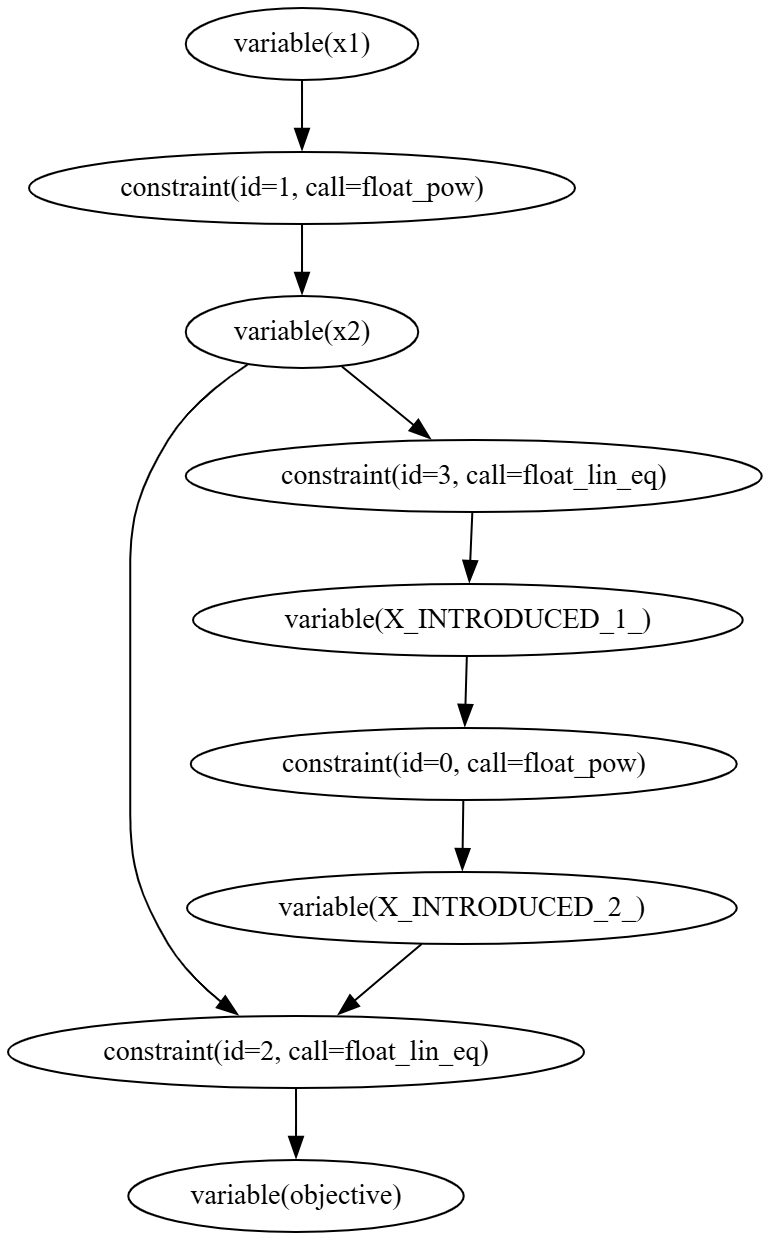
\includegraphics[width=0.4\linewidth]{figures/invariant_graph.png}
	\caption{Example of invariant graph}
	\label{fig:invariant_graph}
\end{figure}

\section{Integrating FlatZinc and PSO}
\label{sec:fzn_integration_pso}

Solving a constraint optimization problem with PSO using the information contained in the FlatZinc model and soft constraints requires associating each built-in FlatZinc function with a corresponding violation function.

In Flatzinc-based PSO, each violation function measures the distance from the feasible region, as this strategy has been shown to be more effective than death-based penalties~\cite{pulido2004constraint, mezura2011constraint}. For instance, the constraint \texttt{float\_pow} is represented in FlatZinc by the built-in function:

\[ \texttt{float\_pow}(\texttt{var float:} x,\texttt{var float:} y, \texttt{var float:} z)\]

\noindent corresponding to the relation $z = x^y$. Its violation can therefore be expressed as:

\[\max\left(|x^y - z|, 0\right)\].

The FlatZinc-based PSO must assign a value to each decision variable identified in the invariant graph $\mathcal{G}$ derived from the MiniZinc model. Therefore, the position of each particle $s \in [1..\swarmsize]$ is represented by an array $p_s$ of dimension $d$, where $d$ is the number of decision variables in $\mathcal{G}$.

Once the particle position $p_s$ has been determined, the values of the defined variables are computed by traversing the constraints in $\mathcal{G}$ according to their topological order, and the violation of each constraint is evaluated using its corresponding violation function.

The overall constraint violation associated with particle $p_s$ is computed as the sum of the violations of all constraints represented in $\mathcal{G}$:

\[
cv(p_s)=\sum_{c\in\mathcal{C}}cv_c(p_s),
\]

\noindent where $\mathcal{C}$ denotes the set of constraints represented in the invariant graph $\mathcal{G}$, and $cv_c(p_s)$ denotes the violation associated with constraint $c$.

\begin{algorithm}[htbp]
	\footnotesize
	\caption{FlatZinc-Based Particle Swarm Optimization initialization phase}
	\label{alg:fzn_pso_pt1}
	\begin{algorithmic}[1]
		\Require Swarm size $\swarmsize$, maximum number of iterations $\maxiter$, inertia weight $w$, cognitive coefficient $c_1$, social coefficient $c_2$, invariant graph $\mathcal{G}$
		\Ensure Best solution found $p^*$
		
		\State Let $d$ be the number of variables identified in $\mathcal{G}$
		\label{alg:start_init}
		
		\For{$s=1$ to $\swarmsize$}
		\State Randomly initialize $p_s$ within the bounds of the variables in $\mathcal{G}$
		\State Randomly initialize velocity vector $v_s$
		\State $k_s\gets0$
		\label{alg:end_init}
		
		\State Evaluate $p_s^*$ computing $cv(p_s^*)$ and $f(p_s^*)$
		\label{alg:init_eval}
		\State $p_s^* \gets p_s$
		\label{alg:start_init_update}
		\If{$cv(p_s^*)=0$}
		\If{$f(p_s^*) < f(p^*)$}
		\State $p^*\gets p_s^*$
		\EndIf
		\ElsIf{$cv(p_s^*) < cv(p^*)$}
		\State $p^*\gets p_s^*$
		\EndIf
		\label{alg:end_init_update}
		
		\EndFor
		\algstore{part1}
	\end{algorithmic}
\end{algorithm}

\begin{algorithm}
	\caption{FlatZinc-Based Particle Swarm Optimization search phase}
	\label{alg:fzn_pso_pt2}
	\begin{algorithmic}[1]
		\algrestore{part1}
		\For{$k=1$ to $\maxiter$}
		\For{$s=1$ to $\swarmsize$}
		
		\For{$i=1$ to $d$}
		\State Randomly generate $r_1,r_2\in[0,1]$
		\label{alg:start_update}
		\State $v_s[i]\gets wv_s[i]+c_1r_1(p_s^*[i]-p_s[i])+c_2r_2(p^*[i]-p_s[i])$
		\label{alg:end_update}
		
		
		\State Randomly generate $\rho\in[0,1]$
		\label{alg:start_noise}
		\If{$\rho<0.5$}
		\State Randomly generate $\epsilon\in[-\delta,\delta]$
		\State $v_s[i]\gets v_s[i]+\epsilon$
		\Comment{Perturbed velocity}
		\EndIf
		\label{alg:end_noise}
		
		\State $p_s[i]\gets p_s[i]+v_s[i]$
		\label{alg:start_second_eval}
		\EndFor
		
		\State Evaluate $p_s$ and compute $cv(p_s)$ and $f(p_s)$
		\label{alg:end_second_eval}
		
		\If{$k_s=k_{\max}$}
		\label{alg:start_stagnation}
		\Comment{Stagnation prevention}
		\State Reinitialize $p_s$ and $v_s$
		\State $p_s^*\gets p_s$
		\State $k_s\gets0$
		\EndIf
		\label{alg:end_stagnation}
		
		\If{$cv(p_s)=0$ \textbf{and} $cv(p_s^*)=0$}
		\label{alg:start_deb}
		\If{$f(p_s) < f(p_s^*)$}
		\State $p_s^*\gets p_s$
		\State $k_s\gets0$
		\If{$f(p_s*) < f(p^*)$}
		\State $p^*\gets p_s^*$
		\EndIf
		\EndIf
		\ElsIf{$cv(p_s) < cv(p_s^*)$}
		\State $p_s^*\gets p_s$
		\State $k_s\gets0$
		\Else
		\State $k_s\gets k_s+1$
		\EndIf
		\label{alg:end_deb}
		
		\EndFor
		
		\EndFor
		
		\State \Return $p^*$
		
	\end{algorithmic}
\end{algorithm}

Algorithms~\ref{alg:fzn_pso_pt1} and~\ref{alg:fzn_pso_pt2} present the pseudocode of the FlatZinc-based PSO. The algorithm takes as input the swarm size $\swarmsize$, the maximum number of iterations $\maxiter$, the inertia weight $w$, the cognitive coefficient $c1$, the social coefficient $c2$, and the invariant graph $\mathcal{G}$ of the FlatZinc model. It returns the best solution found by the swarm, denoted by $p^*$.

At the beginning of the initialization phase in lines~\ref{alg:start_init}--\ref{alg:end_init} of Algorithm~\ref{alg:fzn_pso_pt1}, each particle is initialized from the invariant graph $\mathcal{G}$ by considering the number of decision variables $d$ and their corresponding bounds. The particle position $p_s$ and velocity $v_s$ are randomly initialized, and a stagnation counter $k_s$ is set to zero. The counter tracks the number of consecutive iterations in which the particle fails to improve its personal best. Since strict adherence to Deb's rules can lead to premature convergence, the particle is reinitialized when the counter reaches a predefined threshold, promoting exploration and helping the search escape local optima.

Once the first position is assigned, each particle is evaluated in terms of objective value and constraint violations, as described in line~\ref{alg:init_eval} of Algorithm~\ref{alg:fzn_pso_pt1}. In this phase, the solution proposed by the particle is injected into the invariant graph $\mathcal{G}$ and the values of the defined variables as well as the constraint violations are computed.

At the end of the evaluation (lines~\ref{alg:start_init_update}--\ref{alg:end_init_update} of Algorithm~\ref{alg:fzn_pso_pt1}), the personal best position $p_s^*$ of each particle is set to its first evaluated solution, and the global best solution $p^*$ is updated considering the best candidate found among all particles.

During the search phase, in lines~\ref{alg:start_update}--\ref{alg:end_update} of Algorithm~\ref{alg:fzn_pso_pt2}, the velocity of each particle is iteratively update according to the standard PSO equations. 

In lines~\ref{alg:start_noise}--\ref{alg:end_noise} of Algorithm~\ref{alg:fzn_pso_pt2}, uniformly sampled noise $\epsilon \in (-\delta,\delta)$ is added to the particle velocity when a randomly generated value $\rho$ is below $0.5$. These perturbations allow particles to occasionally deviate from their current trajectories, helping them escape local optima and promoting broader exploration of the search space~\cite{hu2002solving}.

After updating the velocity, the position is updated accordingly, and the particle is evaluated in terms of constraint violation and objective function (lines~\ref{alg:start_second_eval}--\ref{alg:end_second_eval} of Algorithm~\ref{alg:fzn_pso_pt2}).

At the end of the evaluation, the stagnation mechanism is applied. If a particle does not improve its personal best for $k_{\max}$ consecutive iterations, it is reinitialized as described in lines~\ref{alg:start_stagnation}--\ref{alg:end_stagnation} of Algorithm~\ref{alg:fzn_pso_pt2}.

Candidate solutions are compared using Deb's rules, and after updating the personal best positions, the global best solution $p^*$ is updated accordingly as illustrated in lines~\ref{alg:start_deb}--\ref{alg:end_deb}  of Algorithm~\ref{alg:fzn_pso_pt2}. Finally, at the end of the optimization process, the best solution found is returned.


\section{Evaluation}
To evaluate the effectiveness of the proposed integration, the algorithm described in Section~\ref{sec:fzn_integration_pso} was compared with a non-FlatZinc PSO implementation. Both algorithms adopt the same search strategy; the only difference is that the FlatZinc-based PSO derives the variables and constraints from the FlatZinc model, whereas the non-FlatZinc implementation directly encodes the problem variables and constraints in the PSO code.

The two approaches were evaluated on the benchmark problems presented in~\cite{hu2002solving} and~\cite{parsopoulos2002particle}, comprising a total of 15 problems\footnote{Problems 3 and 4 presented in~\cite{parsopoulos2002particle} correspond to problems g09 and g04 presented in~\cite{hu2002solving}, respectively, whereas problem 5 represents a variant of problem 4 for which the solution is unknown.}.The experiments were conducted on a 64-bit Windows machine equipped with an Intel Core i5 processor and 16~GB of RAM. 

To ensure a fair comparison between the two approaches, the hyperparameters were set to those presented in Section~\ref{sec:evaluation}, which were shown to be effective in guiding the PSO search towards high-quality solutions for constraint optimization problems. Since the benchmark problems are less complex and involve fewer constraints than those considered for fixture layout optimization, only the \texttt{swarm\_size} and \texttt{max\_iteration} parameters were reduced, to 100 and 500, respectively.

\begin{table}[t]
	\centering
	\footnotesize
	\caption{Comparison between FlatZinc-based PSO and non-FlatZinc PSO. The best value (closest to the optimum) is highlighted in bold when there is a difference between the values proposed.}
	\label{tab:fzn_pso_comparison}
	\setlength{\tabcolsep}{5pt}
	\begin{tabular}{cccccc}
		\toprule
		\textbf{Problem} & \textbf{Optimum} & \textbf{Best fzn-PSO} & \textbf{Best PSO} & \textbf{Mean fzn-PSO} & \textbf{Mean PSO} \\
		\midrule
		g01 & -15.000 & \textbf{-14.892} & -14.825 & \textbf{-13.025} & -12.887 \\
		\midrule
		g02 & -0.804 & \textbf{-0.345} & -0.341 & -0.281 & \textbf{-0.298} \\
		\midrule
		g03 & -1.000 & \textbf{-0.956} & -0.947 & \textbf{-0.895} & -0.785 \\
		\midrule
		g04 & -30665.386 & \textbf{-30666.331} & -30666.226 & \textbf{-30665.388} & -30664.476 \\
		\midrule
		g05 & 5126.496 & -- & -- & -- & -- \\
		\midrule
		g06 & -6961.813 & -6951.099 & \textbf{-6953.812} & \textbf{-6922.202} & -6904.423 \\
		\midrule
		g07 & 24.306 & \textbf{32.896} & 33.607 & 71.290 & \textbf{47.094} \\
		\midrule
		g08 & 0.095 & -0.096 & -0.096 & -0.096 & -0.096 \\
		\midrule
		g09 & 680.630 & \textbf{684.614} & 685.152 & \textbf{687.721} & 689.371 \\
		\midrule
		g10 & 7049.248 & \textbf{8015.163} & 8283.200 & 12657.795 & \textbf{10026.341} \\
		\midrule
		g11 & 0.750 & \textbf{0.750} & 0.749 & \textbf{0.750} & 0.749 \\
		\midrule
		g12 & -1.000 & -1.000 & -1.000 & -1.000 & -1.000 \\
		\midrule
		problem 1 & 1.393 & 1.999 & \textbf{1.392} & 1.999 & \textbf{1.392} \\
		\midrule
		problem 2 & -6961.813 & -6946.519 & \textbf{-6953.812} & \textbf{-6922.013} & -6904.063 \\
		\midrule
		problem 6 & -213.000 & -211.501 & -211.501 & -211.501 & -211.501 \\
		\bottomrule
	\end{tabular}
\end{table}

Table~\ref{tab:fzn_pso_comparison} presents the results of the comparison between the FlatZinc-based PSO and the non-FlatZinc PSO. The results are evaluated on 50 independent runs for each problem, using the same random seed for both algorithms to ensure identical initial conditions. Results for problem g05 are omitted, as neither algorithm was able to find a feasible solution.

Considering the results reported in the table for the mean, the FlatZinc-based PSO achieves better performance in 7 of the 15 problems, while the two approaches obtain identical results in 3 problems. Among the remaining cases, excluding g05, the non-FlatZinc PSO performs better in 4 problems.

Since both algorithms share the same search mechanism, the observed performance differences can primarily be attributed to the information provided by the FlatZinc model. As described in Section~\ref{sec:flattening}, the flattening process produces a more explicit representation of the original model, decomposing complex constraints and identifying defined variables. This additional information allows constraint violations to be evaluated in greater detail and can reduces the number of variables that must be directly searched.

\begin{table}[t]
	\centering
	\footnotesize
	\caption{Runtime comparison between FlatZinc-PSO and non-FlatZinc PSO.}
	\label{tab:runtime_comparison}
	\setlength{\tabcolsep}{5pt}
	\begin{tabular}{ccc}
		\toprule
		\textbf{Problem} & \textbf{fzn-PSO (ms)} & \textbf{PSO (ms)} \\
		\midrule
		
		g01 & 2260.000 & 1500.000 \\
		\midrule
		
		g02 & 6930.000 & 2510.000 \\
		\midrule
		
		g03 & 2130.000 & 1210.000 \\
		\midrule
		
		g04 & 1660.000 & 626.760 \\
		\midrule
		
		g05 & -- & -- \\
		\midrule
		
		g06 & 984.960 & 265.970 \\
		\midrule
		
		g07 & 3040.000 & 1220.000 \\
		\midrule
		
		g08 & 878.160 & 266.950 \\
		\midrule
		
		g09 & 1900.000 & 864.160 \\
		\midrule
		
		g10 & 1670.000 & 934.520 \\
		\midrule
		
		g11 & 419.950 & 266.350 \\
		\midrule
		
		g12 & 1550.000 & 726.060 \\
		\midrule
		
		problem 1 & 702.450 & 153.410 \\
		\midrule
		
		problem 2 & 874.010 & 265.710 \\
		\midrule
		
		problem 6 & 1210.000 & 698.410 \\
		
		\bottomrule
	\end{tabular}
\end{table}


However, the processing of this additional information comes at the cost of more computational overhead. Table~\ref{tab:runtime_comparison} reports the runtimes, in milliseconds, required by the FlatZinc-based PSO and the non-FlatZinc PSO to complete 500 iterations. On average, the non-FlatZinc PSO is approximately 2.55 times faster than the FlatZinc-based PSO.

To assess whether the observed differences in solution quality are statistically significant, a \emph{Wilcoxon signed-rank test}~\cite{woolson2007wilcoxon} was performed on the results of the 50 runs for each benchmark problem. This test compares two related samples by ranking the absolute differences between paired observations and assessing whether these differences are systematically positive or negative. The resulting $p_{value}$ measures the evidence against the null hypothesis that the two methods produce equivalent results; a value of $p_{value}<0.05$ is considered to indicate a statistically significant difference between the two methods. 

\begin{table}[t]
	\centering
	\footnotesize
	\caption{Wilcoxon signed-rank test p-values comparing FlatZinc PSO and non-Flatzinc PSO across benchmark problems. Values with $p_{value} < 0.05$ are highlighted in bold.}
	\label{tab:wilcoxon_pvalues}
	\setlength{\tabcolsep}{5pt}
	\begin{tabular}{cc}
		\toprule
		\textbf{Problem} & \textbf{Wilcoxon $p_{value}$} \\
		\midrule
		
		g01 & 0.1781 \\
		\midrule
		
		g02 & \textbf{0.001191} \\
		\midrule
		
		g03 & \textbf{2.994e-11} \\
		\midrule
		
		g04 & \textbf{1.867e-07} \\
		\midrule
		
		g05 & -- \\
		\midrule
		
		g06 & \textbf{0.003205} \\
		\midrule
		
		g07 & 0.2115 \\
		\midrule
		
		g08 & \textbf{6.825e-05} \\
		\midrule
		
		g09 & \textbf{0.007844} \\
		\midrule
		
		g10 & \textbf{0.0009504} \\
		\midrule
		
		g11 & \textbf{1.776e-15} \\
		\midrule
		
		g12 & \textbf{8.882e-15} \\
		\midrule
		
		problem 1 & \textbf{1.776e-15} \\
		\midrule
		
		problem 2 & \textbf{0.01026} \\
		\midrule
		
		problem 6 & \textbf{0.005942} \\
		
		\bottomrule
	\end{tabular}
\end{table}

Table~\ref{tab:wilcoxon_pvalues} reports the corresponding $p_{value}$ obtained from the run-by-run comparison of the FlatZinc-based PSO and the non-FlatZinc PSO for the benchmark problems. Overall, statistically significant differences were found for 12 of the 15 benchmark problems considered, indicating that the two approaches produce significantly different solution qualities in the majority of the cases.



	
	\chapter{Conclusion}
	\label{chap:pt1_conclusion}

This first part of the thesis focused on the development of an Intelligent Decision Support System (IDSS) for the fixture layout optimization problem in wood industry.

Several solution strategies were developed and evaluated. Initially, a simplified version of the problem was considered, which did not account for the presence of areas to be extruded within the workpiece and for the rotation of the fixtures. This problem was formulated as a CP model implemented in MiniZinc and evaluated using two alternative objective functions. The first, $\finer$, accounts for the principal moments of inertia of the fixture system, whereas the second, $\fdistsemi$, provides an alternative formulation that approximates $\finer$ by considering the distance and size of the fixtures.

The analysis conducted on a case study showed that $\finer$ is more suitable for identifying optimal fixture layouts, but its computational cost increases substantially with problem complexity. In contrast, $\fdistsemi$ provides good-quality solutions in shorter computation times and is less affected by increasing problem complexity. These results therefore motivated the use of an alternative objective function that approximates the results produced by $\finer$ for exact optimization techniques such as CP or MIP.

The complete problem was subsequently considered, incorporating both the areas to be extruded and the rotation of the fixtures. The CP model was extended and compared with two alternative approaches: a MIP model and a Q-learning based algorithm. Testing the three approaches on real-world case studies, the CP model proved to be the most effective solution, with its effectiveness demonstrated by its ability to obtain optimal solutions for the simpler instances when solved with Chuffed, while the use of $\lns$ enabled it to handle the more complex cases. The MIP model solved with Gurobi produced solutions comparable to those of CP for simpler instances, but its performance deteriorated as the problem complexity increased. Q-learning was able to generate good fixture layouts, but did not outperform the solutions obtained with CP or MIP.

None of these approaches, however, explicitly considered fixture rotation during the optimization process, as including arbitrary rotations directly in the decision variables would substantially increase the search space. Rotation was therefore introduced in a subsequent refinement phase based on the PSO meta-heuristic. Starting from the solutions generated by the three approaches, PSO improved the initial layouts in all test cases and also outperformed the layouts provided by an expert operator, with the exception of one case in which the initial solution was of low quality. These results demonstrate the effectiveness of using local search as a refinement mechanism and highlight the advantage of integrating the approaches, as the initial feasible layouts provide PSO with a suitable starting point without requiring it to search for feasibility from scratch.

The application of PSO to the fixture layout optimization problem relied on the linear constraints of the MIP model, implemented in MiniZinc. However, incorporating these constraints into PSO required them to be explicitly reformulated and integrated in its code. To overcome this limitation and enable PSO to solve MiniZinc models involving continuous variables and nonlinear constraints, a FlatZinc-based PSO algorithm was developed. The algorithm exploits the information contained in the FlatZinc model, obtained form the compilation of the MiniZinc model, and represents its information through an invariant graph, allowing constraint violations and the values of defined variables to be evaluated directly from this representation.

The comparison with a PSO implementation in which the variables and constraints are directly encoded in the meta-heuristic showed that the FlatZinc-based approach can achieve better solution quality while using the same search mechanism. This improvement can therefore be attributed to the additional information provided by the FlatZinc model, which offers a more explicit description of the problem and can be exploited to guide the search.

Overall, the results demonstrate that complex constrained problems arising in industrial applications often benefit from the integration of exact optimization and local search techniques. The results obtained for the fixture layout optimization problem demonstrate the effectiveness of this integration, while the development of the FlatZinc-based PSO extends this approach beyond the specific application considered and opens the possibility of applying PSO to a broader class of nonlinear models formulated in MiniZinc.



	
	\part{Heating Process Optimization}
	
	\chapter{Background}
	\label{chap:pt2_background}
This chapter provides the necessary background to introduce terms and concepts that may be unfamiliar to the reader, thereby facilitating the understanding of the work presented in this second part of the thesis.

\section{Physics Informed Machine Learning}

Informed Machine Learning (IML) refers to a learning paradigm in which learning is guided by a combination of data and prior knowledge. In this paradigm, the prior knowledge is provided by an independent source and explicitly incorporated into the machine learning pipeline~\cite{von2021informed}.

Physics-Informed Machine Learning (PIML) is a specific instance of this paradigm, in which machine learning models are trained to perform learning tasks while incorporating knowledge of the physical laws governing the phenomenon under study.

Prior physical knowledge can be incorporated into a neural network at different stages of the learning process, including the training data, the network architecture or model structure, and the learning algorithm~\cite{faroughi2024physics}. These different integration strategies result in different classes of physics-aware neural networks:

\begin{itemize}
	\item \textit{Physics-Guided Neural Networks} rely on training datasets generated from experiments or numerical simulations that already satisfy the underlying physical laws. In this case, physical knowledge is incorporated implicitly through the data used for training;
	
	\item \textit{Physics-Encoded Neural Networks} incorporate physical knowledge directly into the network architecture or model structure by designing its components and connections according to known physical laws;
	
	\item \textit{Physics-Informed Neural Networks} incorporate physical knowledge into the learning process through the loss function, where governing equations, boundary conditions, or conservation laws are included as additional terms.
\end{itemize}


\section{Forward problem and inverse problem}

In the scientific field, the difference between a forward problem and its inverse lies in the direction of the inference. In the former, the objective is to predict the distribution of observations given known distributions of the initial conditions and model parameters. In the latter, the objective is to infer the distributions of the initial conditions and model parameters from the available observations. Consequently, the inverse problem can be ill-posed when the available observations are insufficient to determine a unique solution.

As illustrated in Figure~\ref{fig:forward_inverse_problem}, in physics, the forward problem can be solved using numerical simulators since the physical laws governing the phenomenon under study are known. When, on the other hand, the inverse problem is considered, this information is not available, and only the observations can be used. Consequently, numerical simulators cannot be directly used to solve the inverse problem, and alternative strategies, such as neural networks, can be adopted.

\begin{figure}[hb]
	\centering
	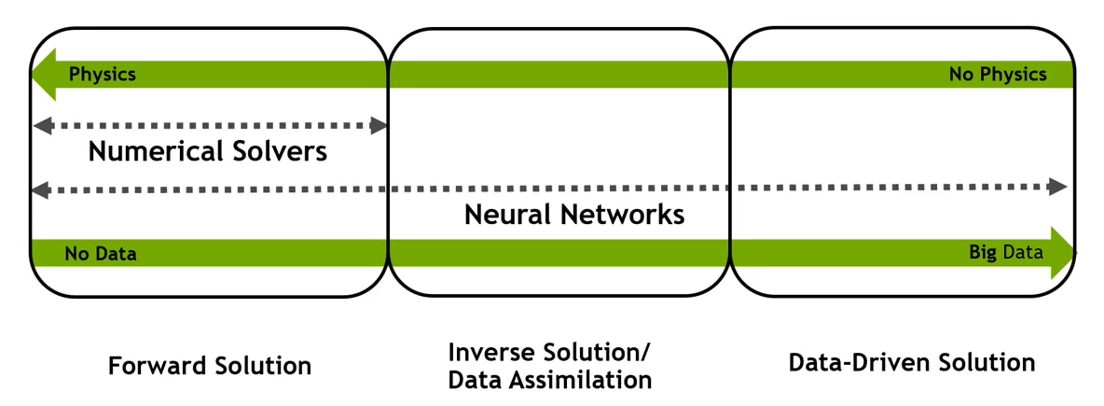
\includegraphics[width=0.8\linewidth]{figures/forward_inverse_problem.png}
	\caption{Solving forward problem and inverse problem}
	\label{fig:forward_inverse_problem}
\end{figure}


	
	\chapter{Introduction}
	\label{pt2:introduction}

\begin{figure}[t]
	\centering
	\begin{subfigure}{0.35\linewidth}
		\centering
		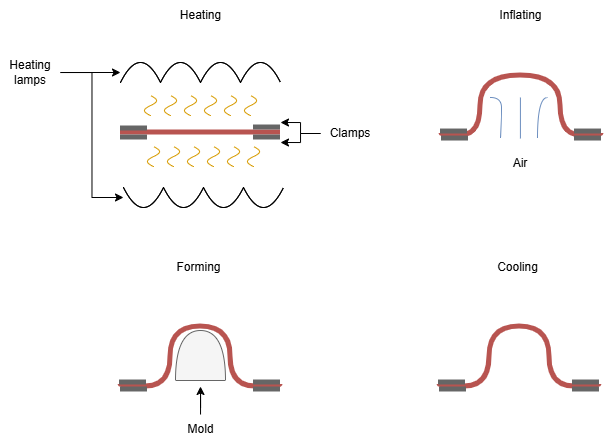
\includegraphics[width=\linewidth]{figures/thermoforming_process.png}
		\caption{The four stages of thermoforming}
		\label{fig:thermoforming_process}
	\end{subfigure}
	\hspace{0.1\linewidth}
	\begin{subfigure}{0.30\linewidth}
		\centering
		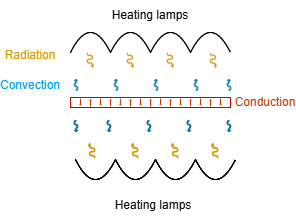
\includegraphics[width=\linewidth]{figures/raditaion_conduction_convection.png}
		\caption{Thermoforming heating phase: conduction, convection, and radiation}
		\label{fig:thermoforming_conduction_convection_radiation}
	\end{subfigure}
	
	\caption{Overview of thermoforming: process stages and heat transfer mechanisms during the heating phase}
	\label{fig:thermoforming_overview}
\end{figure}

Thermoforming is a process in which a plastic sheet is heated and shaped over a mold, transforming it from a rigid to a malleable state~\cite{throne2011thermoforming}. In industrial applications, this process is automated using a thermoforming machine and typically involves four stages: (1) heating, (2) inflating, (3) forming, and (4) cooling, as shown in Figure~\ref{fig:thermoforming_process}. The heating phase is critical for the final product quality: if the sheet temperature is too high, material degradation or sagging may occur, whereas if it is too low, the material may be insufficiently deformable~\cite{schmidt2003modelling,rosen2002thermoforming}.

The final geometry obtained after cooling is strongly influenced by the thermal conditions established during heating, particularly the temperature distribution at the core of the sheet. However, direct measurement of the temperature distribution at the core of the sheet is not feasible in industrial settings, where only surface measurements are typically available.

As shown in Figure~\ref{fig:thermoforming_conduction_convection_radiation} accurate modeling of the heating phase requires accounting for heat conduction within the sheet, convection with the surrounding environment, and radiative exchange between lamps and the sheet. Since radiative heat transfer depends on the fourth power of temperature and on geometric view factors~\cite{bergman2011fundamentals}, high-fidelity numerical models must solve coupled heat transfer equations to predict the temperature distribution within the oven~\cite{turan2025convolutional}. 

Although physics-based simulators that reproduce both machine control logic and heat transfer phenomena can accurately estimate the internal temperature distribution, their computational cost prevents their use in real-time control loops.

\begin{figure}[t]
	\centering
	\begin{subfigure}{0.35\linewidth}
		\centering
		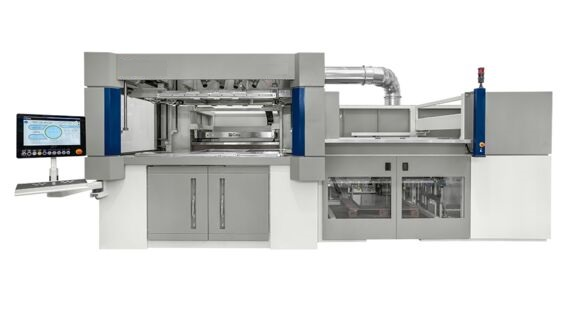
\includegraphics[width=\linewidth]{figures/thermoforming_machine.jpeg}
		\caption{Thermoforming machine}
		\label{fig:thermoforming_machine}
	\end{subfigure}
	\hspace{0.1\linewidth}
	\begin{subfigure}{0.35\linewidth}
		\centering
		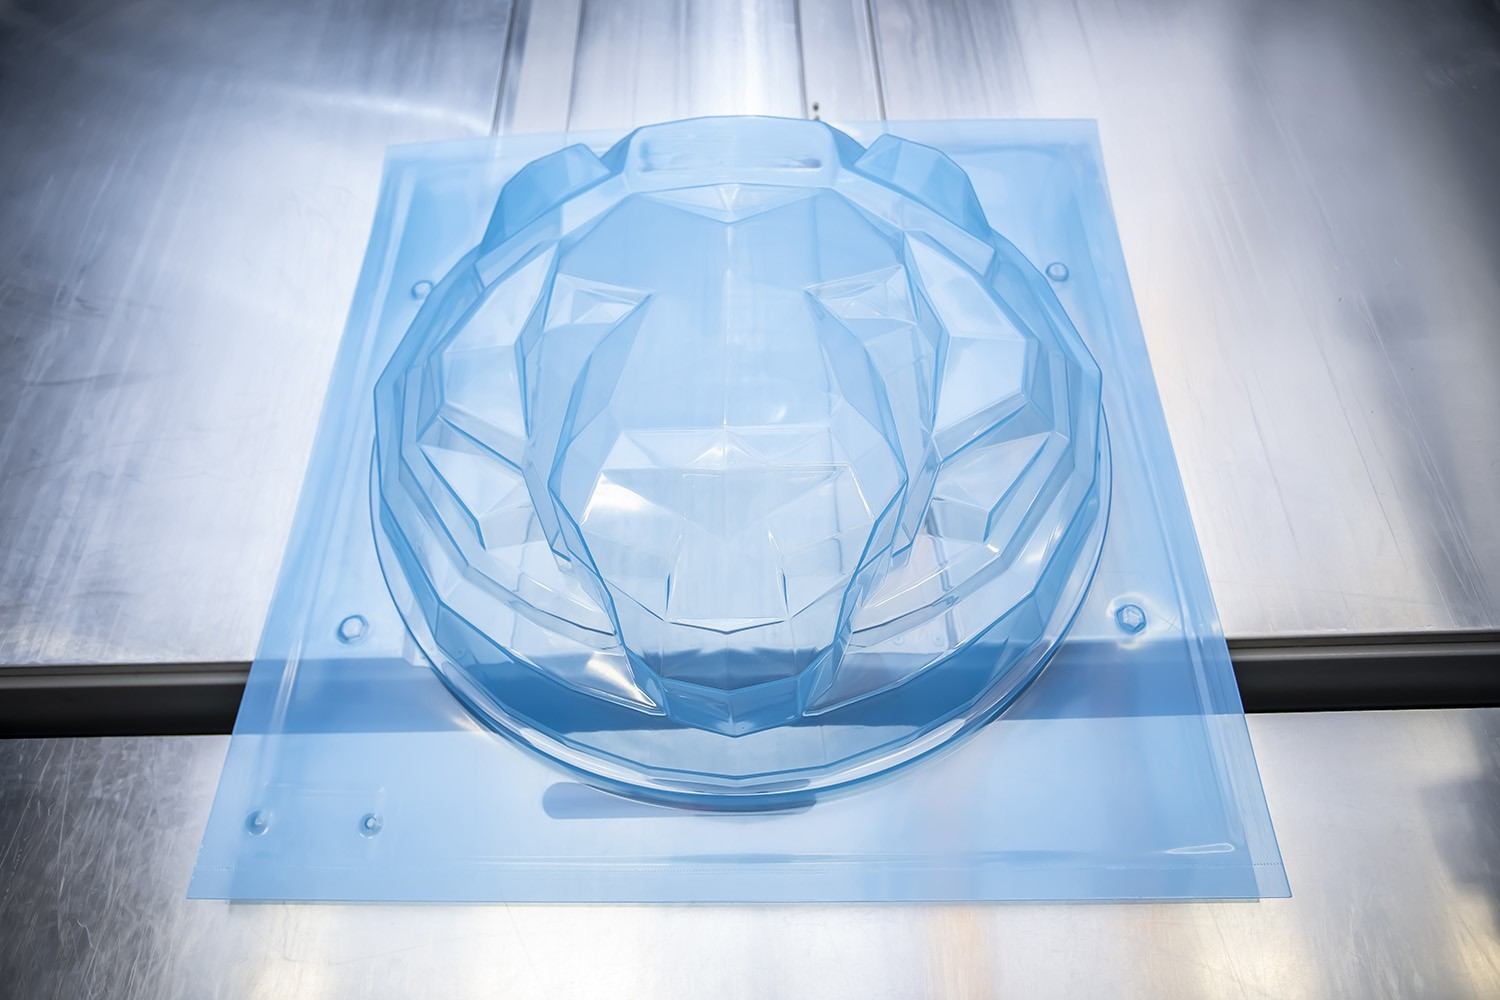
\includegraphics[width=\linewidth]{figures/thermoforming_result.jpg}
		\caption{Thermoformed product result}
		\label{fig:lion_shape}
	\end{subfigure}
	\caption{Thermoforming machine and an example of a thermoformed product obtained at the end of the process}
	\label{fig:thermoforming_combined}
\end{figure}

Given a specific mold geometry, such as the one shown in Figure~\ref{fig:lion_shape}, domain experts aim to apply greater heating to protruding regions of the sheet, which require increased flexibility, while limiting heating in other areas. Experts can therefore qualitatively define a desired core temperature distribution; however, achieving it typically requires multiple trial-and-error iterations to determine suitable machine parameters, resulting in significant time and material waste.

To address these challenges, we propose two artificial neural network (ANN) models. The first is a surrogate model of a physics-based simulator, designed to provide fast and accurate predictions of the temperature distribution at the core of the sheet. This surrogate model is then used to train a second network, an inverse model that predicts machine parameters from a desired temperature distribution while explicitly accounting for process cost.

Although the inverse model can reduce process costs, its predictions may deviate from the target temperature distribution due to the ill-posed nature of the inverse problem, in which different machine parameter configurations may produce similar temperature distributions. Reducing these deviations is important to improve the robustness of the model, which is trained on simulator-generated data and must be applied to real-world cases that may exhibit significant variability in product geometry and forming requirements.

To this end, a targeted optimization step is applied at the level of individual instances. This procedure refines the inverse model solution by reducing the temperature distribution error while adjusting the trade-off between thermal accuracy and process cost.

One of the main challenges in applying data-driven approaches in industrial settings is data scarcity. As noted by Wanigasekara et al.~\cite{wanigasekara2021machine}, thermoforming can be considered a small-data problem due to the high cost and time required for data acquisition. To address this limitation, we generated a dataset using a simulation tool provided by SCM Group S.p.A., which combines a physics-based simulator with a coupled machine control model. A total of \num{18432} samples were generated using \emph{Latin Hypercube Sampling} (LHS)~\cite{loh1996latin}, of which \num{16384} were used for training and 2~048 for validation. The test set consists of 45 real industrial cases collected by the industrial partner during one day of testing.

This study was conducted using an industrial thermoforming machine as reference, shown in Figure~\ref{fig:thermoforming_machine}, equipped with 240 halogen lamps arranged in two grids of 120 elements each, positioned above and below the sheet.

The remainder of this second part of the thesis is organized as follows. Chapter~\ref{chap:pt2_state_of_the_art} presents the state of the art; Chapter~\ref{chap:surrogate_model} presents the surrogate model; Chapter~\ref{chap:inverse_model} describes the inverse model; Chapter~\ref{chap:optimization} introduces the optimization strategy; and Chapter~\ref{chap:pt2_conclusion} concludes this part of the thesis.

	
	\chapter{State of the art}
	\label{chap:pt2_state_of_the_art}

The use of neural networks for solving physical problems has been extensively studied in the literature, particularly following the introduction of Physics-Informed Neural Networks (PINNs) by Raissi et al.~\cite{raissi2019physics}. 

A significant portion of PINN approaches and data-driven methods in thermoforming has focused on inverse modeling strategies aimed at identifying optimal process parameters to reduce defects in the final product geometry. For instance, Yang et al.~\cite{yang2004modeling} proposed an inverse neural network model to predict optimal process conditions for achieving a uniform thickness distribution across the sheet. Chang et al.~\cite{chang2005derivation} developed an inverse model that maps desired product dimensions to process parameters in order to minimize dimensional deviations. Similarly, Leite et al.~\cite{leite2018vacuum} trained a neural network using processing parameters as inputs and defect indicators as outputs, incorporating an optimization objective to reduce forming defects. Tan et al.~\cite{tan2022prediction} employed dual neural networks to infer process parameters from simulation images and optimize them for shear angle uniformity.

More recent studies have shifted attention toward earlier stages of the thermoforming process, particularly the heating phase. Simoncini et al.~\cite{simoncini2017neural} proposed a neural network model to predict polymer behavior under coupled thermal and mechanical effects, with emphasis on infrared heating interactions. Römer et al.~\cite{romer2022temperature} applied reinforcement learning to design a temperature control strategy for the pre-forming stage in automated tape laying processes. Jalilvand et al.~\cite{jalilvand2024towards} used deep reinforcement learning to optimize heating settings for a target temperature distribution, achieving reduced energy consumption. Ayçiçek et al.~\cite{aycciccek2024ai} developed an artificial intelligence-based thermal inspection system using thermal imaging, reducing defects and material waste. Turan et al.~\cite{turan2025convolutional} proposed a surrogate model based on Convolutional Neural Networks (CNNs) and addressed the inverse problem of predicting lamp powers using gradient-based optimization.

Despite these advances, existing approaches either rely on surface temperature information or do not explicitly model the temperature distribution at the core of the sheet, which is critical for product quality. Moreover, these methods often assume simplified industrial conditions, such as uniform sheet properties or single-sided heating configurations, and frequently rely on steady-state assumptions that fail to capture the transient dynamics of the heating phase, limiting their applicability in real industrial environments.

In this study, we address these limitations by explicitly modeling the temperature distribution at the core of the sheet under realistic industrial thermoforming conditions. In contrast to prior work, the proposed method does not rely on steady-state assumptions; instead, it is trained on time-dependent simulations to accurately predict the final temperature distribution.
	
	\chapter{Surrogate model}
	\label{chap:surrogate_model}

The proposed surrogate model $\mathcal{S}$ is designed to approximate the physics-based simulator by learning the mapping from machine parameters and sheet properties to the resulting core temperature distribution. Its objective is to provide accurate and computationally efficient predictions that can be integrated into the heating optimization pipeline.

To capture the spatial information of the thermoforming process, $\mathcal{S}$ is implemented using a \emph{Mesh Graph Neural Network} (MGNN)~\cite{pfaff2020learning}, a class of neural networks capable of producing predictions that account for the mesh structure of the input elements. 

MGNNs operate on a graph representation $G=(V,E)$, where nodes $V$ correspond to mesh vertices and edges $E$ encode local geometric relationships. Each node is associated with a feature vector $x_i$, while each edge feature $e_{ij}$ encodes relative spatial information such as displacement and distance.

\begin{figure}[t]
	\centering
	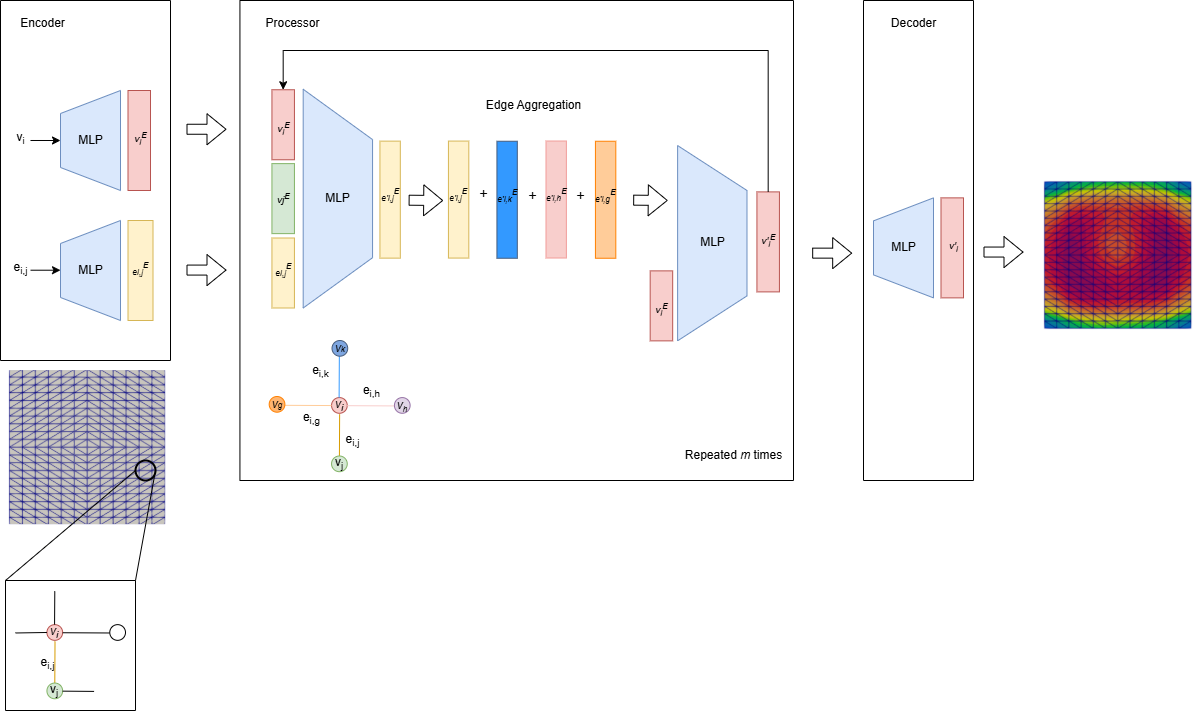
\includegraphics[width=\linewidth]{figures/surrogate_model.png}
	\caption{Mesh Graph Neural Network (MGNN) representing the surrogate model architecture.}
	\label{fig:surrogate_model}
\end{figure}

The MGNN architecture consists of three stages: encoder, processor, and decoder (Figure~\ref{fig:surrogate_model}). During the encoding stage, both node features $x_i$ and edge features $e_{ij}$ are mapped into their respective embedded representations, $v_i^E$ and $e_{ij}^E$. The processor stage performs message passing~\cite{battaglia2018relational} over the graph, where information is exchanged between nodes and their neighbors via the connecting edges over $m$ time steps, leading to iterative updates of the node embeddings $v_i^E$. Finally, in the decoding stage, the updated node embeddings are mapped to the model’s outputs, denoted by $v_i'$, which represent the network’s prediction at mesh vertex $i$.

The input vector of $\mathcal{S}$ consists of 254 features describing mesh node coordinates, sheet geometry (width, height, and thickness), material properties (volumetric heat capacity, emissivity, and thermal conductivity), pyrometer setpoints, lamp powers, and modulation parameters controlling the heating cycle.

The model outputs the predicted core temperature distribution over the mesh vertices together with four process-related quantities: energy consumption, heating time, and the maximum temperatures on the top and bottom surfaces of the sheet.

The encoder consists of two fully connected layers with 512 units, while the decoder consists of two fully connected layers with 128 units. ReLU activations are used throughout. The model is trained using the loss function $\mathcal{L}_s$ defined in Eq.~\ref{eq:loss_surrogate}, optimized with the Adam optimizer~\cite{kingma2014adam} using a learning rate of $1 \times 10^{-3}$ and a batch size of 64. Training is initially set to 1000 epochs, with early stopping applied based on the validation loss, resulting in convergence after 864 epochs.

The training was performed on a workstation equipped with an Intel Core i7 CPU, 16 GB of RAM, and an NVIDIA RTX A4000 GPU, requiring approximately four days.

\section{Loss function formulation}

The loss function adopted for the training of $\mathcal{S}$ balances temperature prediction accuracy and consistency of the process-related outputs. Let $\hat{\mathbf{y}} \in \mathbb{R}^{N \times d}$ denote the predicted outputs and $\mathbf{y}$ the corresponding ground truth, where $N$ is the number of mesh vertices and $d$ is the output dimension. The first component of the output corresponds to the temperature distribution $\hat{\mathbf{y}}_C$, while the remaining $d-1$ components correspond to the process-related outputs. The temperature distribution error is defined as the relative $\ell_2$ norm:

\begin{equation}
	E_T = \frac{\left\| \hat{\mathbf{y}}_C - \mathbf{y}_C \right\|_2}{\left\| \mathbf{y}_C \right\|_2}
\end{equation}

\noindent while the process-related outputs error is computed through the mean squared error:

\begin{equation}
	E_P = \sum_{k=2}^{d} \frac{1}{n} \sum_{i=1}^{n} \left( \hat{\mathbf{y}}_{i,k} - \mathbf{y}_{i,k} \right)^2
\end{equation}

A sigmoid weighting term is used to balance the contributions of $E_T$ and $E_P$ in the final loss:

\begin{equation}
	\sigma = \text{sigmoid} \left( \frac{E_T - \delta}{\tau \cdot \delta} \right)
\end{equation}

\noindent where $\delta = 0.003$ defines the acceptable relative $\ell_2$ error threshold and $\tau = 0.1$ controls the transition sharpness between the two loss regimes, both selected empirically based on preliminary experiments.

The final loss is defined as:

\begin{equation}
	\mathcal{L}_s = \sigma \cdot E_T + (1 - \sigma) \cdot \frac{1}{E_P + 1}
	\label{eq:loss_surrogate}
\end{equation}

This loss formulation adaptively prioritizes temperature distribution accuracy when errors are large, while maintaining consistency with process-related outputs once the temperature prediction is sufficiently accurate.

\section{Model assessment}

\begin{figure}[h]
	\centering
	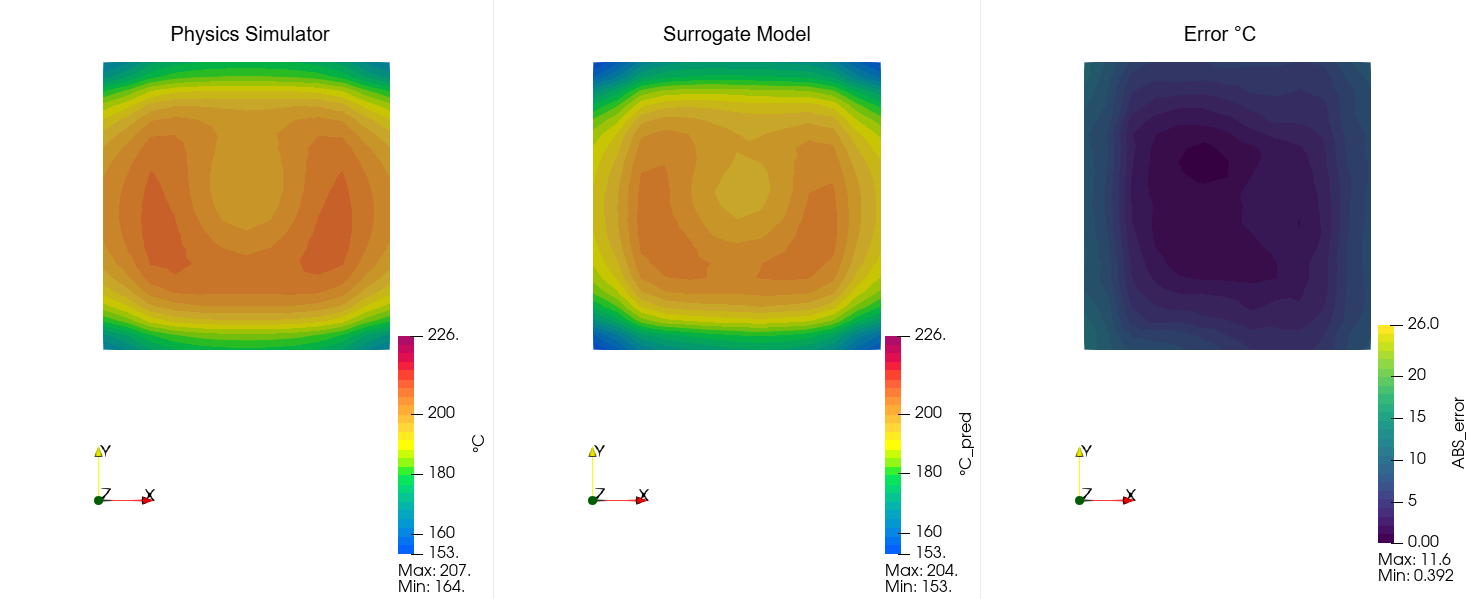
\includegraphics[width=0.7\linewidth]{figures/surrogate_model_with_label.png}
	\caption{Prediction example on the test set. From left to right: the temperature distribution obtained from the physics-based simulator, the prediction produced by the surrogate model and the absolute error between the target temperature distribution and the predicted one.}
	\label{fig:surrogate_model_prediction}
\end{figure}

At the end of training, evaluation of the temperature distribution reveals a maximum average absolute error of $1.23~^\circ\mathrm{C}$ on the training set, $3.43~^\circ\mathrm{C}$ on the validation set, and $9.65~^\circ\mathrm{C}$ on the test set.

Figure~\ref{fig:surrogate_model_prediction} shows an example prediction from the test set. In the example, the surrogate model preserves the spatial structure of the temperature field and correctly identifies regions of higher and lower temperature. The largest deviations occur along the left and right edges of the sheet, where the predicted temperature is slightly lower than the reference solution.

\begin{table}[b]
	\centering
	\footnotesize
	\caption{Physics-based simulator and surrogate model runtime for example.}
	\label{tab:surrogate_perf}
	\setlength{\tabcolsep}{5pt}
	\begin{tabular}{ccc}
		\toprule
		\textbf{Simulator (s)} & \textbf{Surrogate model (s)} & \textbf{Speed-up} \\
		\midrule
		$\approx 105.0$ & $\approx 0.70$ & \textbf{150$\times$} \\
		\bottomrule
	\end{tabular}
\end{table}

Table~\ref{tab:surrogate_perf} reports the processing times required by the physics-based simulator and the surrogate model for a single example. The surrogate model achieves a speed-up of 150$\times$ compared with the physics-based simulator. This reduction in computational time enables its integration into the machine control pipeline and improves the efficiency of training the inverse model, since the loss function is evaluated using temperature distributions generated from the predicted machine parameters.

	
	\chapter{Inverse model}
	\label{chap:inverse_model}

\begin{figure}[ht]
	\centering
	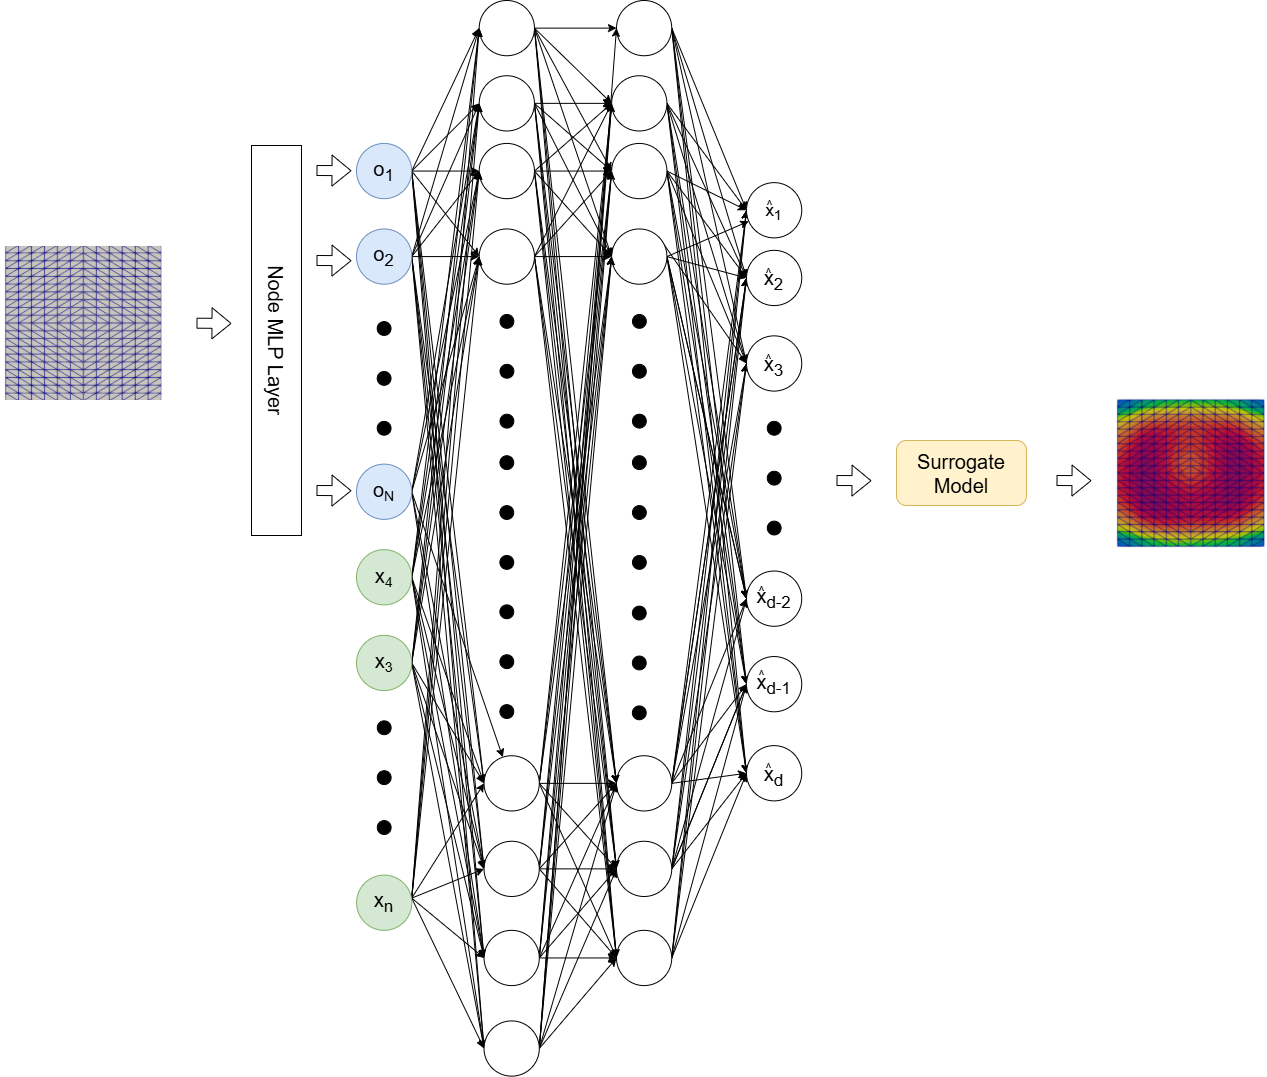
\includegraphics[width=0.6\linewidth]{figures/mesh_mlp.png}
	\caption{Inverse model architecture}
	\label{fig:inverse_model}
\end{figure}


The objective of the inverse model $\mathcal{I}$ is, given a target temperature distribution at the core of the sheet, to infer the machine parameter configuration capable of reproducing it.

In contrast to the surrogate model $\mathcal{S}$, $\mathcal{I}$ does not employ an MGNN architecture, as it is required to output continuous-valued machine parameters that are not inherently associated with mesh nodes, which instead serve as input features.

To preserve the positional temperature information associated with the mesh, the architecture of $\mathcal{I}$ processes node-level information through a Node MLP layer, as illustrated in Figure~\ref{fig:node_mlp}, followed by a fully connected network, as shown in Figure~\ref{fig:inverse_model}.

The input size of the Node MLP layer remains fixed across the dataset. All instances share the same number of mesh nodes, while the mesh is geometrically stretched or compressed according to the sheet geometry of each example.

\begin{figure}[t]
	\centering
	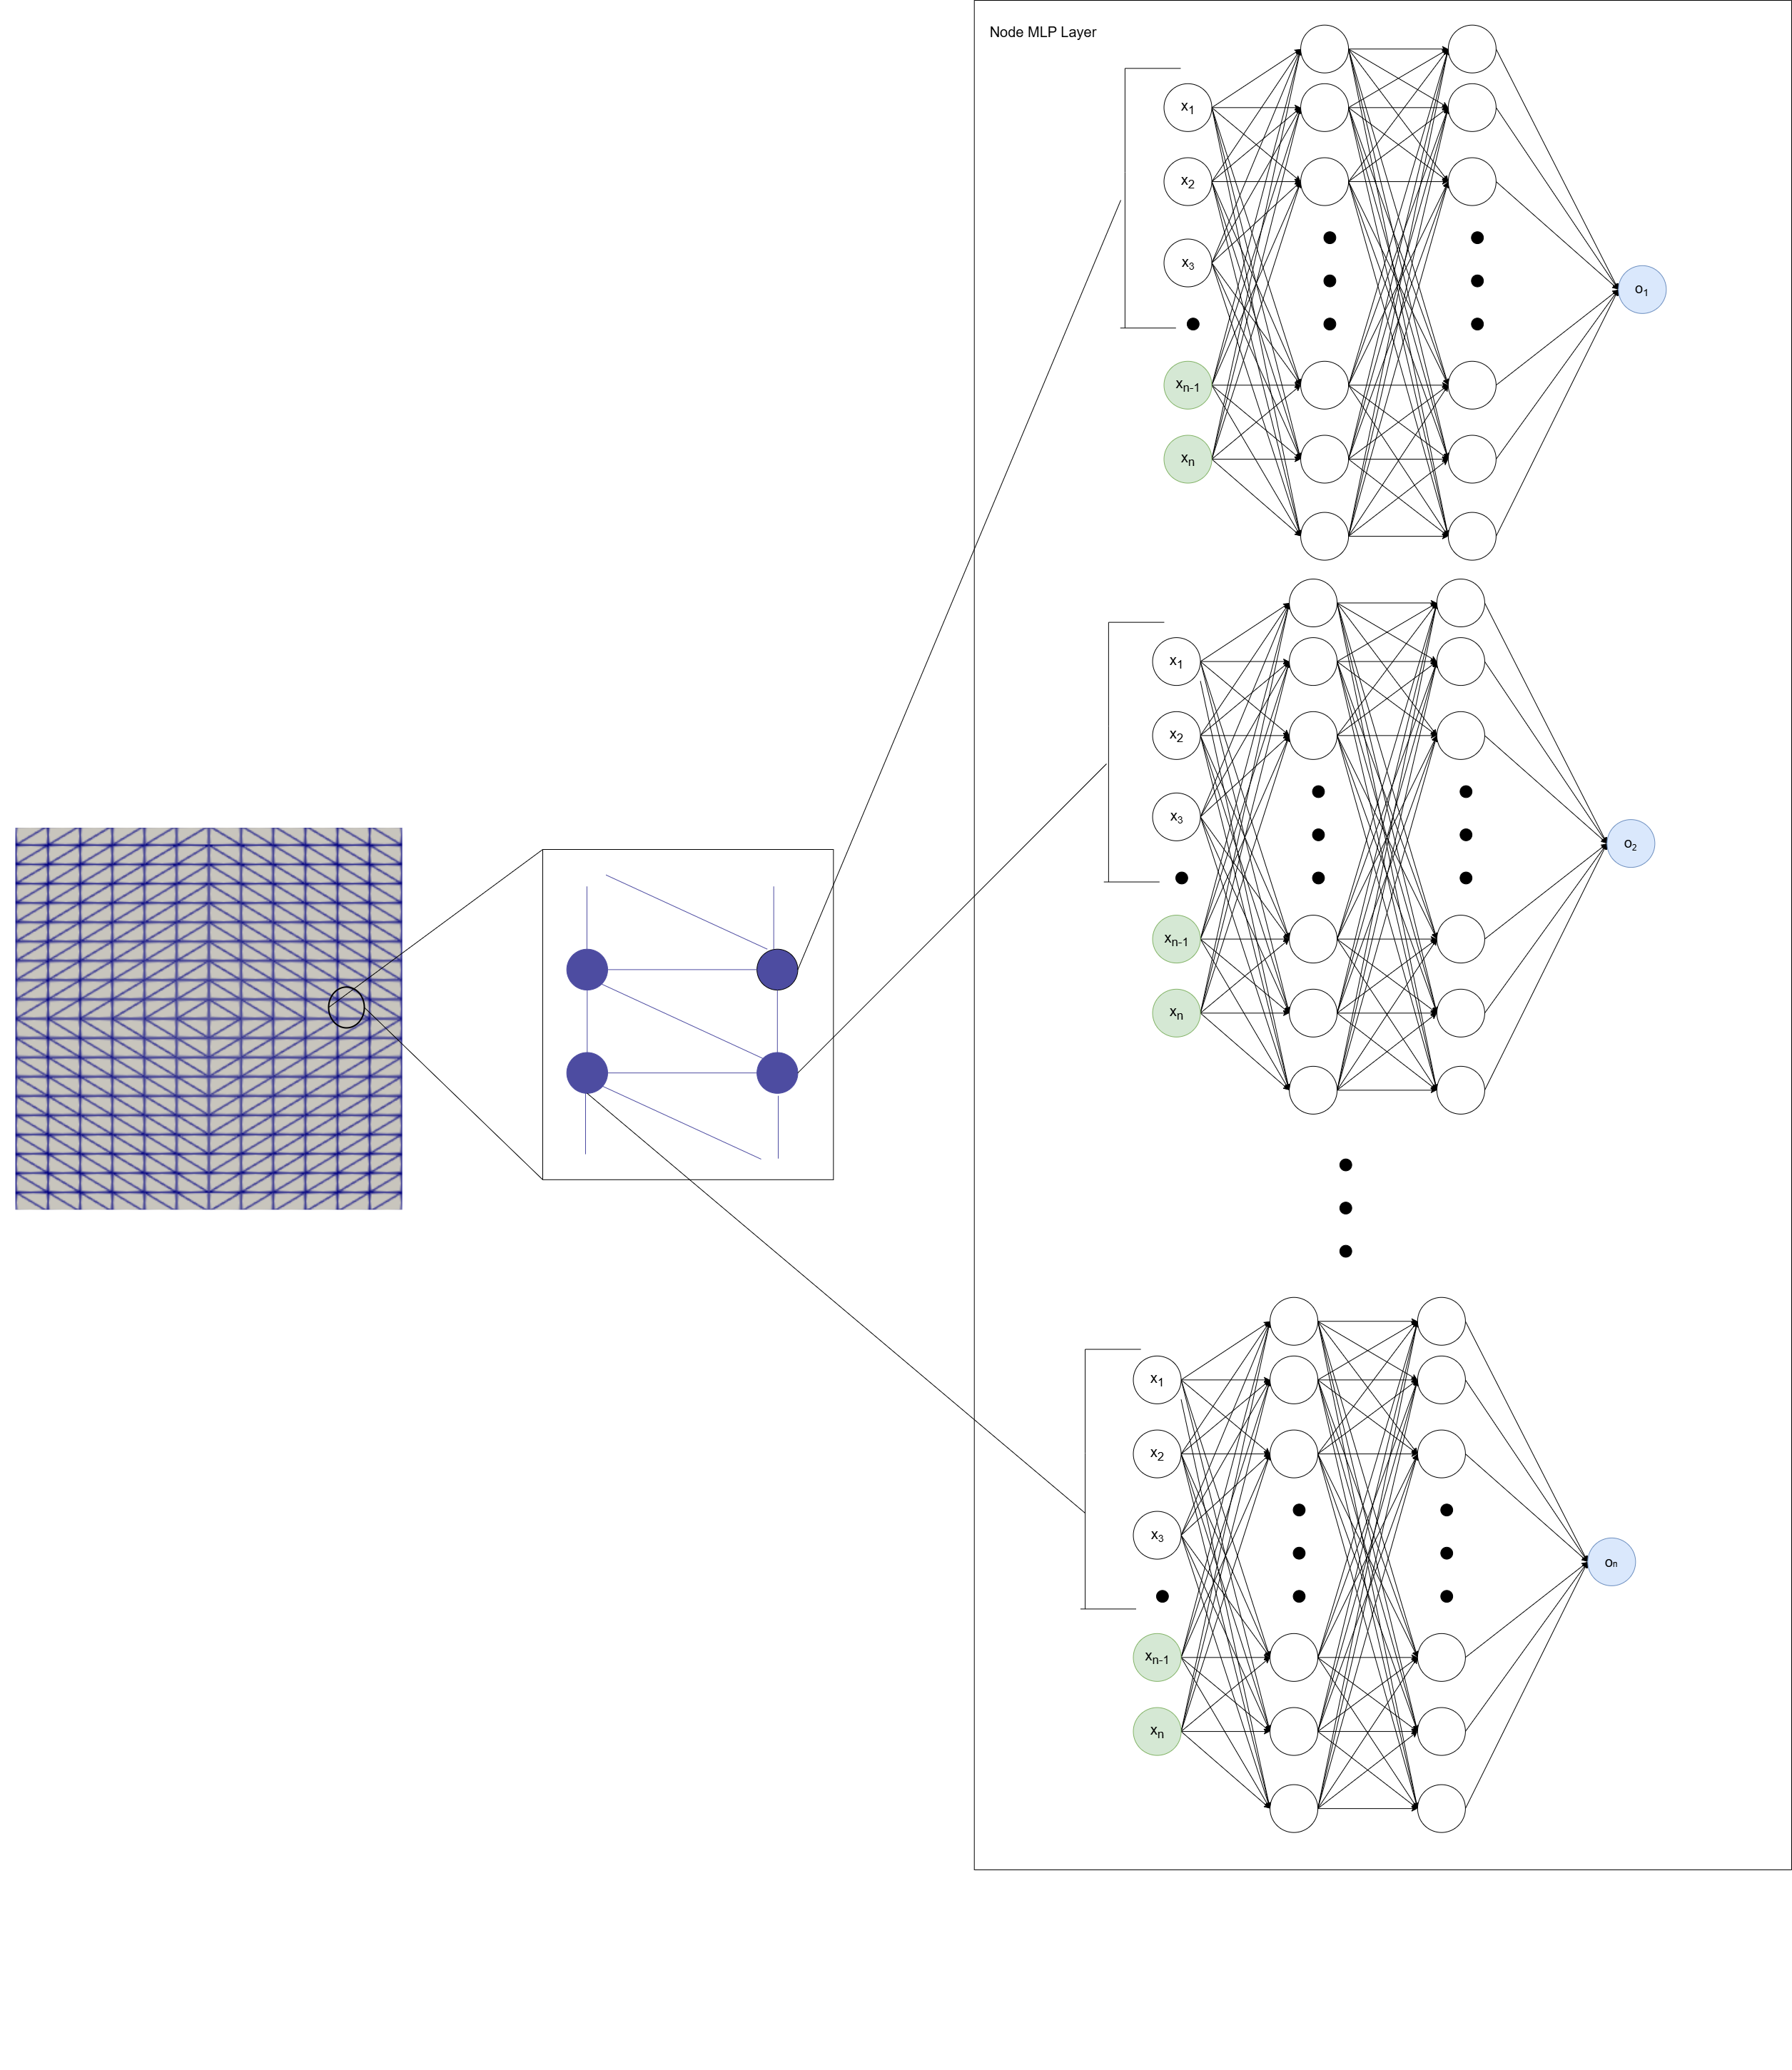
\includegraphics[width=0.5\linewidth]{figures/node_mlp_layer.png}
	\caption{Node MLP layer}
	\label{fig:node_mlp}
\end{figure}

The Node MLP layer consists of a distinct MLP for each mesh node, each composed of two fully connected hidden layers with 16 units. The input to each node-specific MLP includes the mesh node coordinates, the desired temperature at the corresponding node, the sheet geometry (width, height, thickness), and the material properties (volumetric heat capacity, surface emissivity, and thermal conductivity). The sheet characteristics are repeated for each node, as this redundancy has been observed to yield better performance during training than excluding this information.

Each node MLP produces a single output $\mathbf{o}_i$, representing the processed information for node $i$ of the mesh. These outputs are then concatenated with the geometric and material properties of the sheet and processed by a subsequent fully connected network consisting of two hidden layers with 512 units each.

The inverse model predicts a 245-dimensional vector corresponding to the input required by $\mathcal{S}$, excluding the sheet geometry, and material properties, which are shared inputs between both models.

A key component of the output concerns the lamp powers configuration. In the real industrial scenario, machine operators always deactivate lamps outside the sheet area, while setting boundary lamps to the maximum capacity. This prior knowledge is embedded into the model through a masking mechanism applied during training, which prevents updates to the weight corresponding to the already known lamps values, improving convergence stability.

The model is trained using the loss function $\mathcal{L}_i$ expressed in Eq.~\ref{eq:loss_inverse} and optimized using Adam with a learning rate of $1 \times 10^{-2}$. Training is performed with a batch size of 64 for up to 1000 epochs, with early stopping selecting the final model at epoch 842. The training is conducted on the same hardware setup used for the surrogate model and requires approximately four days.

\section{Loss function formulation}
\label{sec:inverse_loss_function}

The inverse problem is inherently ill-posed, since multiple machine configurations may produce similar temperature distributions. Therefore, the objective is not exact reconstruction of simulator inputs, but rather the identification of physically consistent and cost-efficient solutions.

The inverse model prediction $\mathbf{\hat{x}}$ is evaluated through the surrogate model as $\mathbf{\hat{y}} = \mathcal{S}(\mathbf{\hat{x}})$. From the obtained output $\mathbf{\hat{y}}$, we extract the predicted core temperature distribution $\mathbf{\hat{y}}_C$, the maximum temperatures at the top and bottom of the sheet $(\mathbf{\hat{y}}_T, \mathbf{\hat{y}}_B)$, the net heating time $\mathbf{\hat{y}}_H$, and the energy consumption $\mathbf{\hat{y}}_E$.

The temperature error is defined as:
\begin{equation}
	E_T = \frac{1}{n} \sum_{i=1}^{n} \left( \mathbf{\hat{y}}_{C,i} - \left(\mathbf{y}_{C,i} + \frac{\epsilon}{2}\right) \right)^2
\end{equation}

\noindent where $\epsilon = 3~^\circ\mathrm{C}$ defines a temperature tolerance. Shifting the target by $\epsilon/2$ introduces a safety margin that encourages the model to avoid under-heating, which was observed during preliminary experiments.

Process cost is computed as:
\begin{equation}
	P_{\mathrm{Cost}} = \frac{1}{n} \sum_{i=1}^{n} \left( \frac{h}{3600} \mathbf{\hat{y}}_{H,i} + e \mathbf{\hat{y}}_{E,i} \right)
	\label{eq:cost}
\end{equation}

\noindent where $h$ and $e$ are machine-hour cost and energy cost coefficients, respectively.

To ensure material safety constraints, we introduce a penalty term for configurations in which the top surface maximum temperature exceeds the maximum core temperature by more than $\gamma = 15~^\circ\mathrm{C}$:
\begin{equation} 
	\lambda = \frac{1}{n} \sum_{i=1}^{n} \max\left( (\mathbf{\hat{y}}_{T,i} - \mathbf{\hat{y}}^{\max}_{C,i} - \gamma)^2, 0 \right)
	\label{eq:penalty} 
\end{equation}

Only the top surface temperature is considered in this penalty term, as preventing overheating on the top surface, which corresponds to the visible side of the final product, is of primary importance. In contrast, the bottom surface is in contact with the mould during forming and is therefore less critical in terms of thermal degradation.

As for the surrogate model, a sigmoid weighting term balances temperature distribution accuracy and cost minimization:
\begin{equation}
	\sigma = \text{sigmoid} \left( \frac{E_T - \epsilon^2}{\tau \cdot \epsilon^2} \right)
\end{equation}

The final loss is defined as:
\begin{equation}
	\mathcal{L}_i = \sigma E_T + (1 - \sigma) P_{\mathrm{Cost}} + \lambda
	\label{eq:loss_inverse}
\end{equation}

This formulation ensures that the model prioritizes temperature accuracy when errors are significant and progressively shifts its focus toward cost efficiency once thermal targets are sufficiently satisfied, while maintaining safety constraints throughout training.

\section{Model assessment}

\begin{figure}[h]
	\centering
	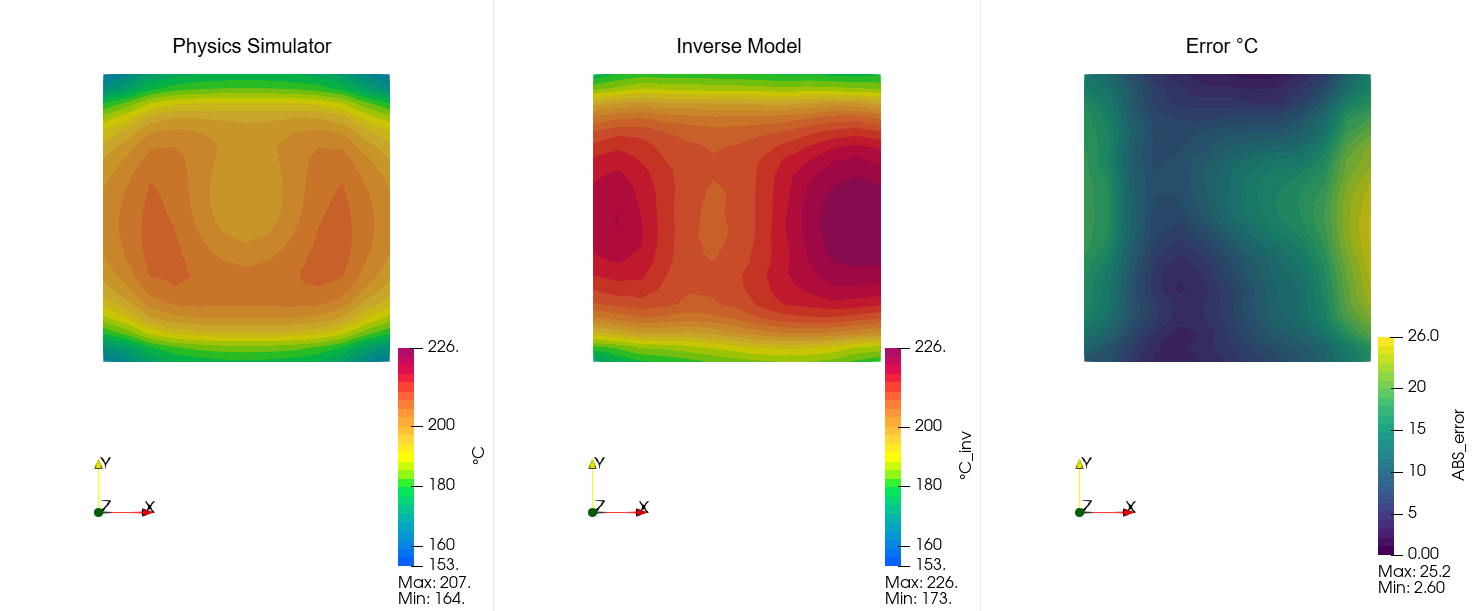
\includegraphics[width=0.7\linewidth]{figures/inverse_model_with_label.png}
	\caption{Prediction example on the test set. From left to right: the temperature distribution obtained from the physics-based simulator, the prediction produced by the inverse model, and the absolute error between the target temperature distribution and the predicted one.}
	\label{fig:inverse_model_prediction}
\end{figure}

At the end of training, evaluation of the temperature distribution revealed a maximum average absolute error of 15.33$^\circ\mathrm{C}$ on the training set, 15.36$^\circ\mathrm{C}$ on the validation set and 22.99$^\circ\mathrm{C}$ on the test set.

Figure~\ref{fig:inverse_model_prediction} illustrates the same test case shown in Figure~\ref{fig:surrogate_model_prediction}, using the inverse model prediction. The model successfully captures the spatial heating strategy, increasing temperatures along the lateral regions while maintaining lower values in the central region and along the top and bottom edges of the sheet.

The error is mainly concentrated on the right-hand side of the sheet, while remaining low in the central and boundary regions. This temperature deviation arises from the inverse model’s tendency to favor higher lamp power configurations, reflecting the learned trade-off between energy usage and processing time, where shorter high-power heating cycles are more cost-efficient than prolonged low-power operation.

Quantitatively, the inverse model achieves an average cost reduction of 49.53\% on the training set, of 49.40\% on the validation set and of 34.52\% on the test set.

Although the results are satisfactory, since the model is trained on simulator-generated data, reducing the temperature deviation with respect to the target distribution is important to improve robustness when applied to real industrial scenarios, where sheet characteristics and operating conditions may vary across cases. 

For this reason, a targeted optimization step is applied at the individual-instance level, starting from the inverse model output. This step primarily reduces the temperature distribution error and subsequently refines the process cost, balancing the trade-off between thermal accuracy and cost minimization.
	
	\chapter{Optimization}
	\label{chap:optimization}

The objective of the optimization procedure is to refine the inverse model prediction by first reducing the temperature distribution error and subsequently minimizing the process cost. The procedure is designed for practical deployment, allowing direct use by the machine operator through an interface exposing the main control parameters.

The optimization procedure implemented is described in Algorithm~\ref{alg:optimizer}. The algorithm uses the Adam optimizer~\cite{kingma2014adam} for 1000 iterations with a learning rate of $1 \times 10^{-1}$. It takes as input the initial parameter values predicted by $\mathcal{I}$, the maximum allowable temperatures for the top and bottom surfaces of the sheet, denoted by $T_\text{T}^{\max}$ and $T_\text{B}^{\max}$, respectively, the machine-hour cost $h$, and the energy cost $e$. The output of the algorithm is the optimized set of machine parameters $\mathbf{x}^{*}$.

The temperature thresholds, together with the machine-hour and energy costs, can be defined by the machine operator based on the material properties, mold geometry, and the cost optimization objective, such as shorter processing times or reduced energy consumption. Since the optimization is performed at the instance level, these values can be specified more precisely for each case, allowing the optimization to better adapt to the specific problem.


\begin{algorithm}[ht]
	\footnotesize
	\caption{Inverse model process parameters optimization}
	\label{alg:optimizer}
	\begin{algorithmic}[1]
		
		\Require Initial machine parameters $\mathbf{\hat{x}}=\mathcal{I}(\mathbf{\hat{y}})$, maximum allowable temperatures $T_\text{T}^{\max}$ and $T_\text{B}^{\max}$, machine-hour cost $h$ and energy cost $e$
		\Ensure Optimized machine parameters $\mathbf{x}^{*}$
		
		\State $I_1 = 500$
		\label{alg:opt_init_start}
		\State $I_2 = 1000$
		\State Initialize the Adam optimizer
		\State Set $\mathbf{x}^{(0)} \gets \mathbf{\hat{x}}$
		\label{alg:opt_init_end}
		
		\For{$k=1$ to $I_1$} \Comment First stage
		\label{alg:opt_first_start}
		\State $\mathbf{\hat{y}} \gets \mathcal{S}(\mathbf{x}^{(k-1)})$
		\State Extract $\mathbf{\hat{y}}_C$, $\mathbf{\hat{y}}_T$, and $\mathbf{\hat{y}}_B$
		\State Compute $E_T^{\max}$ according to Eq.~\ref{eq:max_temp_error}
		\State Compute $\lambda_\text{T}$ and $\lambda_\text{B}$ according to Eq.~\ref{eq:temperature_penalties}
		\State Evaluate objective function $f_{\text{first}}$ according to Eq.~\ref{eq:f_first}
		\State Update of $\mathbf{x}^{(k)}$ by minimizing $f_{\text{first}}$ with Adam
		\EndFor
		\label{alg:opt_first_end}
		

		\For{$k=I_1$ to $I_2$} \Comment Second stage
		\label{alg:opt_second_start}
		\State $\mathbf{\hat{y}} \gets \mathcal{S}(\mathbf{x}^{(k-1)})$
		\State Extract $\mathbf{\hat{y}}_C$, $\mathbf{\hat{y}}_T$, and $\mathbf{\hat{y}}_B$
		\State Compute $E_T^{\max}$ according to Eq.~\ref{eq:max_temp_error}
		\State Compute $\lambda_\text{T}$ and $\lambda_\text{B}$ according to Eq.~\ref{eq:temperature_penalties}
		\State Evaluate objective function $f_{\text{first}}$ according to Eq.~\ref{eq:f_first}
		\State Compute $\sigma$ according to Eq.~\ref{eq:tradeoff_sigmoid}
		\State Evaluate objective function $f_{\text{second}}$ according to Eq.~\ref{eq:f_second}
		\State Update of $\mathbf{x}^{(k)}$ by minimizing $f_{\text{second}}$ with Adam
		\EndFor
		\label{alg:opt_second_end}
		
		\State $\mathbf{x}^{*} \gets \mathbf{x}^{(1000)}$
		\label{alg:opt_output_start}
		\State \textbf{return} $\mathbf{x}^{*}$
		\label{alg:opt_output_end}
		
	\end{algorithmic}
\end{algorithm}

The optimization algorithm is divided into two stages of 500 iterations each. The first stage focuses on reducing the temperature distribution error using Eq.~\ref{eq:f_first} as the objective function. The second stage aims to minimize the process cost while preserving the temperature accuracy achieved in the first stage, using Eq.~\ref{eq:f_second} as the objective function.

In the first-stage of the optimization, during the initialization in lines~\ref{alg:opt_init_start}--\ref{alg:opt_init_end} of Algorithm~\ref{alg:optimizer}, the Adam optimizer is initialized, and the machine parameters predicted by the inverse model $\mathbf{\hat{x}}$, are set as the starting point of the optimization. 

As illustrated in lines~\ref{alg:opt_first_start}--\ref{alg:opt_first_end} of Algorithm~\ref{alg:optimizer}, the surrogate model $\mathcal{S}$ is evaluated for the current machine parameters, and the resulting output prediction are used to compute the temperature error. 

The temperature error considered is computed as the maximum absolute deviation between the predicted and target temperature distributions, incorporating a tolerance margin $\epsilon = 3~^\circ\mathrm{C}$, consistently with the error formulation used in the inverse model (see Section~\ref{sec:inverse_loss_function}):

\begin{equation}
	E_T^{\text{max}} = \max \left| \mathbf{\hat{y}}_C - \left(\mathbf{y}_C + \frac{\epsilon}{2}\right) \right|
\label{eq:max_temp_error}
\end{equation}

\noindent overheating is penalized when the predicted top and bottom temperatures exceed the allowable limits:
\begin{equation}
	\lambda_\text{T} = \max(\mathbf{\hat{y}}_\text{T} - T_\text{T}^{\max}, 0), \quad
	\lambda_\text{B} = \max(\mathbf{\hat{y}}_\text{B} - T_\text{B}^{\max}, 0)
	\label{eq:temperature_penalties}
\end{equation}

The first-stage optimization objective function is defined as:
\begin{equation}
	f_{\text{first}} = E_T^{\text{max}} + \lambda_\text{T} + \lambda_\text{B}.
	\label{eq:f_first}
\end{equation}

During the second stage of the optimization, as reported in lines~\ref{alg:opt_second_start}--\ref{alg:opt_second_end} of Algorithm~\ref{alg:optimizer}, the output obtained from the first-stage is used as the initial input. In this case the objective is to reduce the process cost while preserving the temperature accuracy achieved at the end of the first stage. To this end, a sigmoid function is used to modulate the trade-off between temperature accuracy and process cost minimization:

\begin{equation}
	\sigma = \text{sigmoid} \left( \frac{E_T^{\text{max}} - \epsilon}{\tau \cdot \epsilon} + \lambda_\text{T} + \lambda_\text{B} \right)
	\label{eq:tradeoff_sigmoid}
\end{equation}

The objective function minimized during the second stage is:
\begin{equation}
	f_{\text{second}} = \sigma f_{\text{first}} - (1 - \sigma) \cdot \frac{1}{P_{\text{Cost}}} - \epsilon.
	\label{eq:f_second}
\end{equation}

\noindent where $P_{\text{Cost}}$ is the cost function defined in Eq.~\ref{eq:cost}.

Finally, after completion of the two optimization stages, the resulting machine parameters are returned, as reported in lines~\ref{alg:opt_output_start}--\ref{alg:opt_output_end} of Algorithm~\ref{alg:optimizer}. 

%Unlike the neural network models, which are trained using fixed average cost coefficients across all samples, this formulation allows the machine operator to adjust the relative importance of the cost components $h$ and $e$ in Eq.~\ref{eq:cost} at inference time for each instance, enabling different operational objectives, such as shorter processing times or reduced energy consumption.


\section{Evaluation}

To evaluate the effectiveness of the inverse model initialization, we compare the maximum absolute temperature error obtained after optimization when initialized with the parameters predicted by $\mathcal{I}$ against a random initialization. The analysis is conducted using paired comparisons on both validation and test sets, in order to assess the behavior of the optimizer on both simulated and real data.

The results were obtained by executing the optimization strategy, taking into account the material-specific thresholds indicated in~\cite{schwarzmann2018thermoforming} when selecting the maximum allowable temperatures $T_\text{T}^{\max}$ and $T_\text{B}^{\max}$. To allow for comparison with the results obtained from the inverse model, the values of $h$ and $e$ in Eq.~\ref{eq:cost} were set to the same values used by the inverse model and kept constant across all examples.

On the validation set, initialization from the inverse model yields a lower maximum absolute error than random initialization in 80\% of the cases, with a statistical significance of $p_{value} = 9.132e-54$, computed using the \emph{Wilcoxon signed-rank test}~\cite{woolson2007wilcoxon}. On the test set, this proportion is 67\%, with $p_{value} = 3.015e-5$.

These results indicate that initialization from the inverse model provides a more favorable starting point for the optimization procedure than random initialization. Specifically, after the optimization procedure starting form the inverse model outputs, we achieved a maximum average absolute error of $3.15^\circ\mathrm{C}$ on the validation set and $4.23^\circ\mathrm{C}$ on the test set.

\begin{figure}[t]
	\centering
	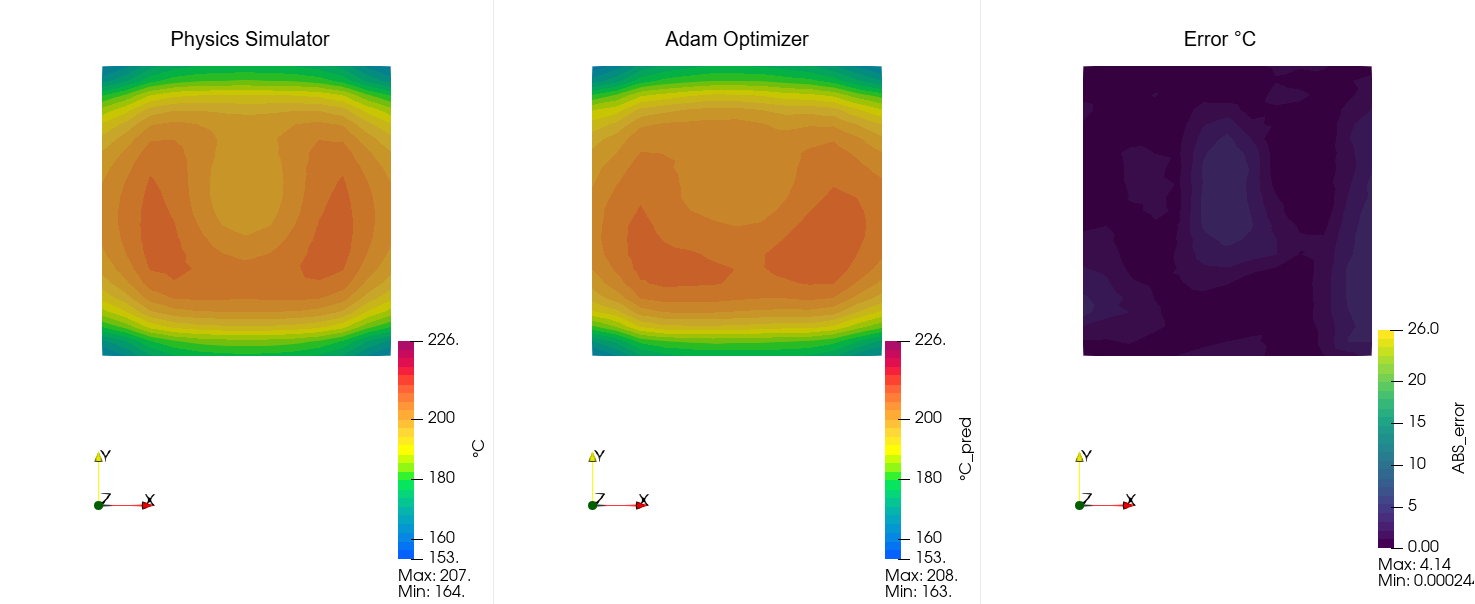
\includegraphics[width=0.7\linewidth]{figures/adam_optimizer_with_label.png}
	\caption{Prediction example on the test set. From left to right: the temperature distribution obtained from the physics-based simulator, the prediction produced by the optimizer, and the absolute error between the target temperature distribution and the predicted one.}
	\label{fig:optimizer_prediction}
\end{figure}

Figure~\ref{fig:optimizer_prediction} illustrates the same example shown in Figure~\ref{fig:surrogate_model_prediction} and Figure~\ref{fig:inverse_model_prediction}, considering the prediction obtained after optimization. The error previously observed along the right-hand side of the sheet is significantly reduced, while the remaining deviations are mainly concentrated in the central region, where the predicted temperature is slightly higher than the target.

The optimizer maintains the tendency to favor higher heating power over shorter durations, reflecting the trade-off learned by the inverse model between energy consumption and processing time. However, compared to the inverse model, the optimization step places greater emphasis on reducing the temperature distribution error by allowing longer heating times. As a result, the additional cost reduction is smaller than that achieved by the inverse model, with a reduction of 11.77\% on the validation set and 8.98\% on the test set.




	
	\chapter{Conclusion}
	\label{chap:pt2_conclusion}

This second part of the thesis presented a data-driven methodology for optimizing the heating phase in thermoforming, considering an industrial thermoforming machine and addressing the inverse problem of determining the machine parameters required to produce a desired core temperature distribution.


The proposed approach relies on two neural network models. A surrogate model based on a Mesh Graph Neural Network (MGNN) is first developed to approximate a physics-based simulator, enabling fast and accurate prediction of the temperature distribution at the core of the sheet. The model achieves a speed-up of approximately $150\times$ with respect to the simulator, while maintaining a maximum average absolute error of $3.43~^\circ\mathrm{C}$ on the validation set and $9.65~^\circ\mathrm{C}$ on the test set.

Building on this model, an inverse model is introduced to predict machine parameters from a target temperature distribution, while incorporating process cost considerations. The model significantly reduces process cost and processing time by favoring higher lamp power configurations that allow the desired thermal state to be reached more quickly. This strategy produces temperature distributions that qualitatively match the desired spatial patterns, but leads to higher predicted temperatures compared to the target distribution. Consequently, the maximum average absolute errors of $15.36~^\circ\mathrm{C}$ on the validation set and $22.99~^\circ\mathrm{C}$ on the test set reflect this trade-off between heating intensity and process duration.

Since the model is trained on simulator-generated data, reducing these temperature deviations is important for improving its robustness when applied to real industrial scenarios, where operating conditions and sheet characteristics may vary significantly between cases.

To this end, a two-stage optimization procedure based on the Adam optimizer is applied to refine the inverse model predictions at the individual sample level. The first stage focuses on reducing the temperature distribution error, while the second improves process cost without degrading thermal accuracy. After optimization, the maximum average absolute error is reduced to $3.15~^\circ\mathrm{C}$ on the validation set and $4.23~^\circ\mathrm{C}$ on the test set, demonstrating an improvement in temperature accuracy that, however, comes at the expense of reduced cost savings compared with the inverse model.

The results highlight the complementary roles of the two components: the inverse model provides satisfactory temperature distributions and cost-efficient initial solutions, while the optimization step refines them by reducing temperature deviations, thereby improving generalization to varying conditions.

The industrial partner has decided to start integrating the proposed strategy into thermoforming machine control workflows and is investigating its potential for extension to support other stages of the thermoforming process.
	
	\chapter{Overall conclusion}
	\label{chap:overall_conclusion}
	
	%----------------------------------------------------------------------------------------
	% BIBLIOGRAPHY
	%----------------------------------------------------------------------------------------
	
	\backmatter
	
	\part*{}
	
	\bibliographystyle{plainnat}
	\bibliography{phd-thesis}
	
\end{document}